\documentclass[12pt,a4paper]{report}
\usepackage[utf8]{inputenc}
\usepackage[english,russian]{babel}
\usepackage{amsmath,amssymb,amsfonts}
\usepackage{bookmark}
\usepackage{geometry}
\usepackage{graphicx}
\usepackage{fancyhdr}
\usepackage{subfiles}
\usepackage{tikz}
\usepackage{pgf,tikz}
\usetikzlibrary{arrows}
\geometry{a4paper, margin=1in}
\usepackage{hyperref}
\hypersetup{
    colorlinks=true,
    linkcolor=blue,
    urlcolor=blue,
    pdftitle={Физика},
    pdfauthor={},
    pdfsubject={},
    pdfkeywords={Определение, формула, законы, процессы},
}

\usepackage{titlesec}
\titleformat{\section}{\Large\bfseries}{\thesection}{1em}{}
\titleformat{\subsection}{\large\bfseries}{\thesubsection}{1em}{}


\setcounter{secnumdepth}{4}
\setcounter{tocdepth}{2}


\renewcommand{\thechapter}{\Roman{chapter}}
\renewcommand{\thesection}{\arabic{section}}
\renewcommand{\thesubsection}{\thesection.\arabic{subsection}}
\renewcommand{\thesubsubsection}{\thesubsection.\arabic{subsubsection}}

\renewcommand{\chaptermark}[1]{\markboth{#1}{}}
\renewcommand{\sectionmark}[1]{\markright{#1}}

% Настройка верхнего колонтитула
\pagestyle{fancy}
\fancyhf{}
\fancyhead[L]{\rightmark} % Левый верхний угол: название главы
\fancyhead[R]{\thepage} % Правый верхний угол: номер страницы
\renewcommand{\headrulewidth}{0.2pt} % Линия под верхним колонтитулом


\begin{document}

\begin{titlepage}
    \centering
    \vspace*{1in}
    {\Huge \textbf{Физика}}\\[2cm]
    \textit{3 семестр}\\[0.5cm]
\end{titlepage}
\tableofcontents

\newpage
\chapter{Механика}
\section{Объекты классической механики}
\begin{itemize}
    \item \textbf{Определение: \textit{Материальная точка}} - это тело, размерами которого можно пренебречь по сравнению с его пространственным перемещением.
    \item \textbf{Определение: \textit{Система материальных точек}} - это множество материальных точек, положение и движение каждой из которых зависит от положения и движения остальных точек множества.
    \item \textbf{Определение: \textit{Абсолютно твердое тело}} - тело, деформациями которого можно пренебречь по сравнению с его пространственным перемещением.
    \item \textbf{Определение: \textit{Сплошная среда}} - всюду плотное множество материальных точек (жидкость, газы, деформируемые твердые тела).
\end{itemize}

\vspace{5px}

\underline{\textbf{Три постулата классической физики}}
\begin{enumerate}
    \item Считается возможным одновременное измерение с любой точностью всех физических величин, описывающих данное тело.
    \item Во всех системах отсчета промежуток времени между двумя событиями считается одинаковым.
    \item Во всех системах отсчета расстояние между двумя телами в данный момент времени считается одинаковым.
\end{enumerate}

\underline{\textbf{Разделы классической механики}}

\vspace{5px}

\textbf{Определение: \textit{Кинематика}} --- раздел механики, который изучает перемещение тел друг относительно друга без учета причин, вызывающих это движение.

\vspace{5px}

\textbf{Определение: \textit{Статика}} --- раздел механики, который изучает условия равновесие тел.

\vspace{5px}

\textbf{Определение: \textit{Динамика}} --- раздел механики, который изучает механическое движение тел с учетом причин, вызывающих это движение.

\vspace{3px}

\section{Кинематика}
\subsection{Кинематика материальной точки}
\textbf{Определение: \textit{Траектория}} --- линия, по которой движется материальная точка.

\vspace{5px}

\textbf{Определение: \textit{Радиус-вектор}} --- вектор, соединяющий тело отсчета с материальной точкой. Обозначается $\vec r$.

\vspace{5px}

\textbf{Определение: \textit{Вектор перемещения (или перемещение)}} --- вектор, соединяющий начальное положение материальной точки с ее текущим положением. Обозначается $\Delta \vec r$.

\vspace{5px}

\textbf{Определение: \textit{Путь}} - полное расстояние, пройденное точкой по траектории. Величина пути всегда неотрицательна. Обозначается s.

\vspace{5px}

\textbf{Способы задания движения точки в пространстве}
\begin{enumerate}
    \item \underline{Векторный} : задаются тело отсчета и радиус-вектор точки в зависимости от времени $\vec r(t)$.
    \item \underline{Координатный:} задаются точка отсчета, система координат, координаты точки в зависимости от времени x(t), y(t), z(t).

          Взаимосвязь между 1 и 2 способами: $\vec r = (x; y; z).$
          \begin{center}
              \begin{tikzpicture}[line cap=round,line join=round,>=triangle 45,x=0.3518393327685422cm,y=0.2826623149406189cm]
                  \clip(5.34,4.59) rectangle (25.4,32.48);
                  \draw [->] (12,16) -- (12,30);
                  \draw [->] (12,16) -- (24,16);
                  \draw [->] (12,16) -- (6.1,10.4);
                  \draw [dash pattern=on 2pt off 2pt] (12,28)-- (18,24);
                  \draw [dash pattern=on 2pt off 2pt] (18,24)-- (18,12);
                  \draw [dash pattern=on 2pt off 2pt] (18,12)-- (7.8,12.01);
                  \draw [dash pattern=on 2pt off 2pt] (18,12)-- (22,16);
                  \draw [dash pattern=on 2pt off 2pt] (12,16)-- (18,24);
                  \draw (11.68,30.09) node[anchor=north west] {\textit{z}};
                  \draw (23.54,15.89) node[anchor=north west] {$y$};
                  \draw (6.49,11.09) node[anchor=north west] {$x$};
                  \draw (9.69,28.61) node[anchor=north west] {$z(t)$};
                  \draw (22.36,18.13) node[anchor=north west] {$x(t)$};
                  \draw (5.83,14.14) node[anchor=north west] {$y(t)$};
                  \draw [dash pattern=on 2pt off 2pt] (12,16)-- (18,12);
                  \draw (11.75,15.62) node[anchor=north west] {$O$};
                  \begin{scriptsize}
                      \fill [color=black] (12,16) circle (1.5pt);
                      \fill [color=black] (18,24) circle (1.5pt);
                      \draw[color=black] (18.23,24.38) node {$M$};
                  \end{scriptsize}
              \end{tikzpicture}
          \end{center}
    \item \underline{Естественный:} задаются траектория движения, начальное положение точки на траектории, положительное направление движения по траектории, координата точки на траектории в зависимости от времени s(t) (причем такая функция должна быть непрерывна и дифференцируема).

          \begin{center}
              \begin{tikzpicture}[line cap=round,line join=round,>=triangle 45,x=0.5173695954768815cm,y=0.2188192609703325cm]
                  \clip(5.02,36.37) rectangle (21.59,59.41);
                  \draw [->] (12,16) -- (12,30);
                  \draw [->] (12,16) -- (24,16);
                  \draw [->] (12,16) -- (6.1,10.4);
                  \draw [dash pattern=on 1pt off 1pt] (12,28)-- (18,24);
                  \draw [dash pattern=on 1pt off 1pt] (18,24)-- (18,12);
                  \draw [dash pattern=on 1pt off 1pt] (18,12)-- (7.8,12.01);
                  \draw [dash pattern=on 1pt off 1pt] (18,12)-- (22,16);
                  \draw [dash pattern=on 1pt off 1pt] (12,16)-- (18,24);
                  \draw (11.69,30.03) node[anchor=north west] {\textit{z}};
                  \draw (23.55,15.85) node[anchor=north west] {$y$};
                  \draw (6.49,11) node[anchor=north west] {$x$};
                  \draw (9.71,28.55) node[anchor=north west] {$z(t)$};
                  \draw (22.36,18.07) node[anchor=north west] {$x(t)$};
                  \draw (5.84,14.07) node[anchor=north west] {$y(t)$};
                  \draw [dash pattern=on 1pt off 1pt] (12,16)-- (18,12);
                  \draw (11.79,15.67) node[anchor=north west] {$O$};
                  \draw [shift={(9.3,50.58)}] plot[domain=-0.13:3.92,variable=\t]({1*3.46*cos(\t r)+0*3.46*sin(\t r)},{0*3.46*cos(\t r)+1*3.46*sin(\t r)});
                  \draw [shift={(16.42,49.48)}] plot[domain=-3.32:0.01,variable=\t]({1*3.75*cos(\t r)+0*3.75*sin(\t r)},{0*3.75*cos(\t r)+1*3.75*sin(\t r)});
                  \draw (10.33,56.24) node[anchor=north west] {$M_0$};
                  \draw (16.03,48.17) node[anchor=north west] {$M$};
                  \draw (15.87,44.9) node[anchor=north west] {$S(t)$};
                  \draw (11.73,52.02) node[anchor=north west] {$+$};
                  \draw (7.83,53.77) node[anchor=north west] {$-$};
                  \draw [->] (9.81,53.27) -- (8.43,53.39);
                  \draw [->] (10.47,52.89) -- (11.75,51.77);
                  \begin{scriptsize}
                      \fill [color=black] (12,16) circle (1.5pt);
                      \fill [color=black] (18,24) circle (1.5pt);
                      \draw[color=black] (5.12,59.58) node {$M$};
                      \fill [color=black] (10.51,53.82) circle (1.5pt);
                      \fill [color=black] (16.26,45.73) circle (1.5pt);
                  \end{scriptsize}
              \end{tikzpicture}
          \end{center}


\end{enumerate}
\subsection{Кинематические элементы движения точки}
\begin{enumerate}
    \item \textbf{Определение: \textit{Скорость --- векторная величина, характеризующая быстроту изменения положения точки в пространстве.}}
          \begin{center}


              \definecolor{qqqqff}{rgb}{0,0,1}
              \definecolor{xdxdff}{rgb}{0.49,0.49,1}
              \begin{tikzpicture}[line cap=round,line join=round,>=triangle 45,x=0.48682970473423426cm,y=0.3773490309806699cm]
                  \clip(32.93,68.72) rectangle (42.68,78.36);
                  \draw [->] (12,16) -- (12,30);
                  \draw [->] (12,16) -- (24,16);
                  \draw [->] (12,16) -- (6.1,10.4);
                  \draw [dash pattern=on 1pt off 1pt] (12,28)-- (18,24);
                  \draw [dash pattern=on 1pt off 1pt] (18,24)-- (18,12);
                  \draw [dash pattern=on 1pt off 1pt] (18,12)-- (7.8,12.01);
                  \draw [dash pattern=on 1pt off 1pt] (18,12)-- (22,16);
                  \draw [dash pattern=on 1pt off 1pt] (12,16)-- (18,24);
                  \draw (11.69,30.03) node[anchor=north west] {\textit{z}};
                  \draw (23.55,15.85) node[anchor=north west] {$y$};
                  \draw (6.49,11) node[anchor=north west] {$x$};
                  \draw (9.71,28.55) node[anchor=north west] {$z(t)$};
                  \draw (22.36,18.07) node[anchor=north west] {$x(t)$};
                  \draw (5.84,14.07) node[anchor=north west] {$y(t)$};
                  \draw [dash pattern=on 1pt off 1pt] (12,16)-- (18,12);
                  \draw (11.79,15.67) node[anchor=north west] {$O$};
                  \draw [shift={(37.64,72.37)}] plot[domain=0.31:2.77,variable=\t]({1*4.99*cos(\t r)+0*4.99*sin(\t r)},{0*4.99*cos(\t r)+1*4.99*sin(\t r)});
                  \draw (33.94,78.13) node[anchor=north west] {$M_0$};
                  \draw (40.78,77.76) node[anchor=north west] {$M$};
                  \draw (34.57,76.3)-- (40.92,76.13);
                  \draw (40.92,76.13)-- (37.52,69.39);
                  \draw (37.52,69.39)-- (34.57,76.3);
                  \draw (34.71,73.29) node[anchor=north west] {$\vec r_0$};
                  \draw (40.33,73.46) node[anchor=north west] {$\vec r$};
                  \draw (37.34,75.41) node[anchor=north west] {$\Delta \vec r$};
                  \begin{scriptsize}
                      \fill [color=black] (12,16) circle (1.5pt);
                      \fill [color=black] (18,24) circle (1.5pt);
                      \draw[color=black] (30.28,81.88) node {$M$};
                      \fill [color=xdxdff] (34.57,76.3) circle (1.5pt);
                      \fill [color=xdxdff] (40.92,76.13) circle (1.5pt);
                      \fill [color=qqqqff] (37.52,69.39) circle (1.5pt);
                  \end{scriptsize}
              \end{tikzpicture}


          \end{center}

          \begin{enumerate}
              \item \underline{Векторный способ:} фиксирует быстроту изменения положения материальной точки.

                    \[ \vec v(cp) = \frac{\Delta \vec r}{\Delta \vec t} \]

                    Рассмотрим \[\lim_{\Delta t \to 0}  \frac{\Delta \vec r}{\Delta t} = \frac{d\vec r}{dt}\]

                    Получим скорость в исследуемый момент времени, так как $v = \frac{d\vec r}{dt} = \dot{r}$ - первая производная радиус вектора $\vec r$ по времени.

              \item \underline{Координатный способ:} $\vec v(v_x, v_y, v_z)$, где $v_x, v_y, v_z$ - скорость вдоль оси X, Y, Z или проекция вектора скорости на оси X, Y, Z соответственно.

                    Соотнося формулы получаем:

                    Так как $\vec r = (x,y,z)$, то
                    \[ v_x = \frac{dx}{dt} = \dot{x} \]
                    \[ v_y = \frac{dy}{dt} = \dot{y} \]
                    \[ v_z = \frac{dz}{dt} = \dot{z} \]

                    Величина скорости - есть длина вектора $\vec v$, а именно : $\sqrt{v_x^2 + v_y^2+v_z^2}$
                    \newpage
              \item \underline{Естественный способ:}

                    \begin{center}
                        \definecolor{qqqqff}{rgb}{0,0,1}
                        \definecolor{xdxdff}{rgb}{0.49,0.49,1}
                        \begin{tikzpicture}[line cap=round,line join=round,>=triangle 45,x=1.0cm,y=0.4462136542823525cm]
                            \clip(39.38,121.82) rectangle (47.61,127.24);
                            \draw [->] (12,16) -- (12,30);
                            \draw [->] (12,16) -- (24,16);
                            \draw [->] (12,16) -- (6.1,10.4);
                            \draw [dash pattern=on 1pt off 1pt] (12,28)-- (18,24);
                            \draw [dash pattern=on 1pt off 1pt] (18,24)-- (18,12);
                            \draw [dash pattern=on 1pt off 1pt] (18,12)-- (7.8,12.01);
                            \draw [dash pattern=on 1pt off 1pt] (18,12)-- (22,16);
                            \draw [dash pattern=on 1pt off 1pt] (12,16)-- (18,24);
                            \draw (11.69,30.03) node[anchor=north west] {\textit{z}};
                            \draw (23.55,15.85) node[anchor=north west] {$y$};
                            \draw (6.49,11) node[anchor=north west] {$x$};
                            \draw (9.71,28.55) node[anchor=north west] {$z(t)$};
                            \draw (22.36,18.07) node[anchor=north west] {$x(t)$};
                            \draw (5.84,14.07) node[anchor=north west] {$y(t)$};
                            \draw [dash pattern=on 1pt off 1pt] (12,16)-- (18,12);
                            \draw (11.79,15.67) node[anchor=north west] {$O$};
                            \draw [shift={(37.64,72.37)}] plot[domain=0.31:2.77,variable=\t]({1*4.99*cos(\t r)+0*4.99*sin(\t r)},{0*4.99*cos(\t r)+1*4.99*sin(\t r)});
                            \draw (33.94,78.13) node[anchor=north west] {$M_0$};
                            \draw (40.78,77.76) node[anchor=north west] {$M$};
                            \draw (34.57,76.3)-- (40.92,76.13);
                            \draw (40.92,76.13)-- (37.52,69.39);
                            \draw (37.52,69.39)-- (34.57,76.3);
                            \draw (34.71,73.29) node[anchor=north west] {$\vec r_0$};
                            \draw (40.33,73.46) node[anchor=north west] {$\vec r$};
                            \draw (37.34,75.41) node[anchor=north west] {$\Delta \vec r$};
                            \draw [shift={(42.31,123.73)}] plot[domain=0.06:3.01,variable=\t]({1*2.39*cos(\t r)+0*2.39*sin(\t r)},{0*2.39*cos(\t r)+1*2.39*sin(\t r)});
                            \draw [shift={(45.92,124.26)}] plot[domain=-2.83:0.07,variable=\t]({1*1.28*cos(\t r)+0*1.28*sin(\t r)},{0*1.28*cos(\t r)+1*1.28*sin(\t r)});
                            \draw [->] (42.13,126.11) -- (45.1,123.27);
                            \draw [dash pattern=on 1pt off 1pt] (45.1,123.27)-- (46.66,122.07);
                            \draw (41.85,127.41) node[anchor=north west] {$M_0$};
                            \draw (42.33,124.62) node[anchor=north west] {$\Delta \vec r$};
                            \draw (45.28,124.52) node[anchor=north west] {$M$};
                            \begin{scriptsize}
                                \fill [color=black] (12,16) circle (1.5pt);
                                \fill [color=black] (18,24) circle (1.5pt);
                                \draw[color=black] (36.65,130.28) node {$M$};
                                \fill [color=xdxdff] (34.57,76.3) circle (1.5pt);
                                \fill [color=xdxdff] (40.92,76.13) circle (1.5pt);
                                \fill [color=qqqqff] (37.52,69.39) circle (1.5pt);
                                \fill [color=black] (42.13,126.11) circle (1.5pt);
                                \fill [color=black] (45.1,123.27) circle (0.5pt);
                            \end{scriptsize}
                        \end{tikzpicture}
                    \end{center}


                    Рассмотрим
                    \[ \vec v = \lim_{\Delta t \to 0}  \frac{\Delta \vec r}{\Delta t}\]
                    Вектор скорости всегда направлен по касательной к траектории в момент времени.

                    Рассмотрим величину скорости:
                    \[ v = \lvert \vec v \rvert =\lvert \lim_{\Delta t \to 0}  \frac{\Delta \vec r}{\Delta t} \rvert =  \lim_{\Delta t \to 0}  \frac{\lvert \Delta \vec r \rvert}{\Delta t} = \lim_{\Delta t \to 0}  \frac{\Delta s}{\Delta t} = \frac{ds}{dt} = \dot s \]

                    \begin{center}
                        \definecolor{qqqqff}{rgb}{0,0,1}
                        \definecolor{xdxdff}{rgb}{0.49,0.49,1}
                        \begin{tikzpicture}[line cap=round,line join=round,>=triangle 45,x=0.7049525857040535cm,y=0.5549198628861888cm]
                            \clip(38.45,122.49) rectangle (48.62,129.23);
                            \draw [->] (12,16) -- (12,30);
                            \draw [->] (12,16) -- (24,16);
                            \draw [->] (12,16) -- (6.1,10.4);
                            \draw [dash pattern=on 1pt off 1pt] (12,28)-- (18,24);
                            \draw [dash pattern=on 1pt off 1pt] (18,24)-- (18,12);
                            \draw [dash pattern=on 1pt off 1pt] (18,12)-- (7.8,12.01);
                            \draw [dash pattern=on 1pt off 1pt] (18,12)-- (22,16);
                            \draw [dash pattern=on 1pt off 1pt] (12,16)-- (18,24);
                            \draw (11.69,30.03) node[anchor=north west] {\textit{z}};
                            \draw (23.55,15.85) node[anchor=north west] {$y$};
                            \draw (6.49,11) node[anchor=north west] {$x$};
                            \draw (9.71,28.55) node[anchor=north west] {$z(t)$};
                            \draw (22.36,18.07) node[anchor=north west] {$x(t)$};
                            \draw (5.84,14.07) node[anchor=north west] {$y(t)$};
                            \draw [dash pattern=on 1pt off 1pt] (12,16)-- (18,12);
                            \draw (11.79,15.67) node[anchor=north west] {$O$};
                            \draw [shift={(37.64,72.37)}] plot[domain=0.31:2.77,variable=\t]({1*4.99*cos(\t r)+0*4.99*sin(\t r)},{0*4.99*cos(\t r)+1*4.99*sin(\t r)});
                            \draw (33.94,78.13) node[anchor=north west] {$M_0$};
                            \draw (40.78,77.76) node[anchor=north west] {$M$};
                            \draw (34.57,76.3)-- (40.92,76.13);
                            \draw (40.92,76.13)-- (37.52,69.39);
                            \draw (37.52,69.39)-- (34.57,76.3);
                            \draw (34.71,73.29) node[anchor=north west] {$\vec r_0$};
                            \draw (40.33,73.46) node[anchor=north west] {$\vec r$};
                            \draw (37.34,75.41) node[anchor=north west] {$\Delta \vec r$};
                            \draw [shift={(43.66,124.16)}] plot[domain=0.04:3.18,variable=\t]({1*3.67*cos(\t r)+0*3.67*sin(\t r)},{0*3.67*cos(\t r)+1*3.67*sin(\t r)});
                            \draw [dash pattern=on 1pt off 1pt] (40.01,122.87)-- (40,128);
                            \draw [->] (40,124) -- (43.61,127.82);
                            \draw [->] (40,124) -- (46.05,126.94);
                            \draw [->] (40,124) -- (41.53,127.14);
                            \draw [->] (40,124) -- (40,126.26);
                            \draw (43.08,129.38) node[anchor=north west] {$\Delta S$};
                            \draw (43.44,125.41) node[anchor=north west] {$\Delta \vec r$};
                            \draw (39.04,125.69) node[anchor=north west] {$\vec \tau$};
                            \begin{scriptsize}
                                \fill [color=black] (12,16) circle (1.5pt);
                                \fill [color=black] (18,24) circle (1.5pt);
                                \draw[color=black] (35.9,134.75) node {$M$};
                                \fill [color=xdxdff] (34.57,76.3) circle (1.5pt);
                                \fill [color=xdxdff] (40.92,76.13) circle (1.5pt);
                                \fill [color=qqqqff] (37.52,69.39) circle (1.5pt);
                            \end{scriptsize}
                        \end{tikzpicture}
                    \end{center}
                    Таким образом, величина скорости определяется производной по времени, направленной по касательной, где сама касательная определена единичным вектором $\vec \tau$, то есть \[ \vec v = \vec \tau \cdot \dot s \] где $\vec \tau$ - вектор, скользящий по одной прямой и не $const$.
          \end{enumerate}
    \item \textbf{\textit{Ускорение (быстрота изменения скорости)}}
          \begin{enumerate}
              \item \underline{Векторный способ:} \[ w = \frac{dv}{dt} = \dot{v} = \ddot r\]
              \item \underline{Координатный способ:} \[ \vec w(w_x, w_y, w_z)\]
                    \[ w_x = \dot v_x = \ddot x \]
                    \[ w_y = \dot v_y = \ddot y\]
                    \[ w_z = \dot v_z = \ddot z\]

                    \[ w = \sqrt{w_x^2 + w_y^2+w_z^2} \]

                    \newpage
                    \section{Краткие сведения из дифференциальной геометрии}
                    \begin{center}
                        \definecolor{uququq}{rgb}{0.25,0.25,0.25}
                        \definecolor{qqqqff}{rgb}{0,0,1}
                        \definecolor{xdxdff}{rgb}{0.49,0.49,1}
                        \begin{tikzpicture}[line cap=round,line join=round,>=triangle 45,x=0.6632682838606465cm,y=0.5100115157177547cm]
                            \clip(38.38,148.04) rectangle (47.29,154.16);
                            \draw [->] (12,16) -- (12,30);
                            \draw [->] (12,16) -- (24,16);
                            \draw [->] (12,16) -- (6.1,10.4);
                            \draw [dash pattern=on 1pt off 1pt] (12,28)-- (18,24);
                            \draw [dash pattern=on 1pt off 1pt] (18,24)-- (18,12);
                            \draw [dash pattern=on 1pt off 1pt] (18,12)-- (7.8,12.01);
                            \draw [dash pattern=on 1pt off 1pt] (18,12)-- (22,16);
                            \draw [dash pattern=on 1pt off 1pt] (12,16)-- (18,24);
                            \draw (11.69,29.99) node[anchor=north west] {\textit{z}};
                            \draw (23.54,15.8) node[anchor=north west] {$y$};
                            \draw (6.51,10.99) node[anchor=north west] {$x$};
                            \draw (9.71,28.52) node[anchor=north west] {$z(t)$};
                            \draw (22.37,18.04) node[anchor=north west] {$x(t)$};
                            \draw (5.85,14.04) node[anchor=north west] {$y(t)$};
                            \draw [dash pattern=on 1pt off 1pt] (12,16)-- (18,12);
                            \draw (11.81,15.71) node[anchor=north west] {$O$};
                            \draw [shift={(37.64,72.37)}] plot[domain=0.31:2.77,variable=\t]({1*4.99*cos(\t r)+0*4.99*sin(\t r)},{0*4.99*cos(\t r)+1*4.99*sin(\t r)});
                            \draw (33.95,78.11) node[anchor=north west] {$M_0$};
                            \draw (40.77,77.73) node[anchor=north west] {$M$};
                            \draw (34.57,76.3)-- (40.92,76.13);
                            \draw (40.92,76.13)-- (37.52,69.39);
                            \draw (37.52,69.39)-- (34.57,76.3);
                            \draw (34.72,73.26) node[anchor=north west] {$\vec r_0$};
                            \draw (40.33,73.44) node[anchor=north west] {$\vec r$};
                            \draw (37.33,75.38) node[anchor=north west] {$\Delta \vec r$};
                            \draw [shift={(43.66,124.16)}] plot[domain=0.04:3.18,variable=\t]({1*3.67*cos(\t r)+0*3.67*sin(\t r)},{0*3.67*cos(\t r)+1*3.67*sin(\t r)});
                            \draw [dash pattern=on 1pt off 1pt] (40.01,122.87)-- (40,128);
                            \draw [->] (40,124) -- (43.61,127.82);
                            \draw [->] (40,124) -- (46.05,126.94);
                            \draw [->] (40,124) -- (41.53,127.14);
                            \draw [->] (40,124) -- (40,126.26);
                            \draw (43.08,129.35) node[anchor=north west] {$\Delta S$};
                            \draw (43.44,125.38) node[anchor=north west] {$\Delta \vec r$};
                            \draw (39.03,125.67) node[anchor=north west] {$\vec \tau$};
                            \draw [shift={(41.4,149.72)}] plot[domain=0.37:3.27,variable=\t]({1*2.18*cos(\t r)+0*2.18*sin(\t r)},{0*2.18*cos(\t r)+1*2.18*sin(\t r)});
                            \draw [shift={(45.77,151.29)}] plot[domain=3.47:5.24,variable=\t]({1*2.45*cos(\t r)+0*2.45*sin(\t r)},{0*2.45*cos(\t r)+1*2.45*sin(\t r)});
                            \draw [->] (40.71,153.9) -- (41.54,148.71);
                            \draw [->] (39,151.55) -- (43.83,152.32);
                            \draw (40.46,152.83) node[anchor=north west] {$M$};
                            \draw (41.67,152.9) node[anchor=north west] {$\vec \tau$};
                            \draw (41.47,151.16) node[anchor=north west] {$\vec n$};
                            \draw (43.7,151.45) node[anchor=north west] {$M_1$};
                            \draw (44.94,150) node[anchor=north west] {$M_2$};
                            \begin{scriptsize}
                                \fill [color=black] (12,16) circle (1.5pt);
                                \fill [color=black] (18,24) circle (1.5pt);
                                \draw[color=black] (37.94,156.42) node {$M$};
                                \fill [color=xdxdff] (34.57,76.3) circle (1.5pt);
                                \fill [color=xdxdff] (40.92,76.13) circle (1.5pt);
                                \fill [color=qqqqff] (37.52,69.39) circle (1.5pt);
                                \fill [color=black] (41.04,151.87) circle (1.5pt);
                                \fill [color=uququq] (43.44,150.5) circle (1.5pt);
                                \fill [color=black] (44.81,149.03) circle (1.5pt);
                            \end{scriptsize}
                        \end{tikzpicture}

                        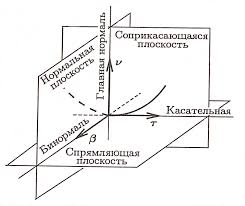
\includegraphics[]{images.jpeg}
                    \end{center}
                    \vspace{5px}

                    --- \textbf{Определение:} Предельное положение плоскости проходящее через точки $M_1,M_2$ некоторой траектории при стремлении $M_1,M_2 \to M$ называется \textbf{\textit{соприкасающейся плоскостью}}.

                    \vspace{5px}

                    --- \textbf{Определение:} Предельное положение прямой проходящей через точки $M,M_1$ при $M_1 \to M$ называется \textbf{\textit{касательной к траектории в точке M}}.Касательная лежит в соприкасающейся плоскости.

                    \vspace{5px}

                    --- \textbf{Определение:} Плоскость перпендикулярная касательной называется \textbf{\textit{нормальной}}.

                    \vspace{5px}

                    --- \textbf{Определение:} Прямая перпендикулярная касательной и лежащая в соприкасающейся плоскости называется \textbf{\textit{главной нормалью.}}

                    \vspace{5px}

                    --- \textbf{Определение:} Прямая перпендикулярная касательной и главной нормали называется \textbf{\textit{би-нормалью}}.

                    \vspace{5px}

                    \textit{$\tau$ выбирают в направлении движения точки, единичный вектор нормали $\vec n$ направлен в сторону вогнутости траектории, а единичный вектор $\vec b$ - би-нормаль направлен так, чтобы $\vec \tau, \vec n, \vec b$ образовывали правую тройку веторов.}

                    \vspace{5px}

                    --- \textbf{Определение:} Плоскость проходящая через касательную и би-нормаль называется \textbf{\textit{спрямляющей плоскостью}}.

                    \vspace{5px}

                    --- \textbf{Определение:} Набор векторов $\vec \tau, \vec n, \vec b$ носит название \textbf{\textit{естественного трехгранника}}.


                    \begin{center}
                        \definecolor{qqwuqq}{rgb}{0,0.39,0}
                        \definecolor{xdxdff}{rgb}{0.49,0.49,1}
                        \begin{tikzpicture}[line cap=round,line join=round,>=triangle 45,x=1.0cm,y=0.8478959000681695cm]
                            \clip(39.05,145.94) rectangle (50.34,152.51);
                            \draw [shift={(47.32,151.4)},color=qqwuqq,fill=qqwuqq,fill opacity=0.1] (0,0) -- (-41.04:0.55) arc (-41.04:0.61:0.55) -- cycle;
                            \draw [->] (12,16) -- (12,30);
                            \draw [->] (12,16) -- (24,16);
                            \draw [->] (12,16) -- (6.1,10.4);
                            \draw [dash pattern=on 1pt off 1pt] (12,28)-- (18,24);
                            \draw [dash pattern=on 1pt off 1pt] (18,24)-- (18,12);
                            \draw [dash pattern=on 1pt off 1pt] (18,12)-- (7.8,12.01);
                            \draw [dash pattern=on 1pt off 1pt] (18,12)-- (22,16);
                            \draw [dash pattern=on 1pt off 1pt] (12,16)-- (18,24);
                            \draw (11.69,29.99) node[anchor=north west] {\textit{z}};
                            \draw (23.54,15.8) node[anchor=north west] {$y$};
                            \draw (6.51,10.99) node[anchor=north west] {$x$};
                            \draw (9.71,28.52) node[anchor=north west] {$z(t)$};
                            \draw (22.37,18.04) node[anchor=north west] {$x(t)$};
                            \draw (5.85,14.04) node[anchor=north west] {$y(t)$};
                            \draw [dash pattern=on 1pt off 1pt] (12,16)-- (18,12);
                            \draw (11.81,15.71) node[anchor=north west] {$O$};
                            \draw [shift={(37.64,72.37)}] plot[domain=0.31:2.77,variable=\t]({1*4.99*cos(\t r)+0*4.99*sin(\t r)},{0*4.99*cos(\t r)+1*4.99*sin(\t r)});
                            \draw (33.95,78.11) node[anchor=north west] {$M_0$};
                            \draw (40.77,77.73) node[anchor=north west] {$M$};
                            \draw (34.57,76.3)-- (40.92,76.13);
                            \draw (40.92,76.13)-- (37.52,69.39);
                            \draw (37.52,69.39)-- (34.57,76.3);
                            \draw (34.72,73.26) node[anchor=north west] {$\vec r_0$};
                            \draw (40.33,73.44) node[anchor=north west] {$\vec r$};
                            \draw (37.33,75.38) node[anchor=north west] {$\Delta \vec r$};
                            \draw [shift={(43.66,124.16)}] plot[domain=0.04:3.18,variable=\t]({1*3.67*cos(\t r)+0*3.67*sin(\t r)},{0*3.67*cos(\t r)+1*3.67*sin(\t r)});
                            \draw [dash pattern=on 1pt off 1pt] (40.01,122.87)-- (40,128);
                            \draw [->] (40,124) -- (43.61,127.82);
                            \draw [->] (40,124) -- (46.05,126.94);
                            \draw [->] (40,124) -- (41.53,127.14);
                            \draw [->] (40,124) -- (40,126.26);
                            \draw (43.08,129.35) node[anchor=north west] {$\Delta S$};
                            \draw (43.44,125.38) node[anchor=north west] {$\Delta \vec r$};
                            \draw (39.03,125.67) node[anchor=north west] {$\vec \tau$};
                            \draw(42.33,148.15) ellipse (1.89cm and 1.6cm);
                            \draw [shift={(42.13,147.3)}] plot[domain=0.32:3.37,variable=\t]({1*2.73*cos(\t r)+0*2.73*sin(\t r)},{0*2.73*cos(\t r)+1*2.73*sin(\t r)});
                            \draw [shift={(46.52,148.54)}] plot[domain=3.35:5.92,variable=\t]({1*1.84*cos(\t r)+0*1.84*sin(\t r)},{0*1.84*cos(\t r)+1*1.84*sin(\t r)});
                            \draw [->] (47.32,151.4) -- (49.44,151.43);
                            \draw [->] (47.32,151.4) -- (49.24,149.73);
                            \draw [->] (42.18,150.03) -- (44.27,150.16);
                            \draw [->] (42.33,148.15) -- (42.18,150.03);
                            \draw [->] (44.06,149.23) -- (45.55,147.95);
                            \draw (48.07,151.52) node[anchor=north west] {$\Delta \Theta$};
                            \draw (48.04,152.51) node[anchor=north west] {$\vec \tau_1$};
                            \draw (47.54,150.77) node[anchor=north west] {$\vec \tau_2$};
                            \draw (44.78,149.55) node[anchor=north west] {$\vec \tau_2$};
                            \draw (42.53,149.51) node[anchor=north west] {$\rho$};
                            \draw (42.97,151.22) node[anchor=north west] {$\vec \tau_1$};
                            \draw (41.91,151.54) node[anchor=north west] {$M$};
                            \draw (44.34,150.3) node[anchor=north west] {$M_1$};
                            \begin{scriptsize}
                                \fill [color=black] (12,16) circle (1.5pt);
                                \fill [color=black] (18,24) circle (1.5pt);
                                \draw[color=black] (38.8,156.71) node {$M$};
                                \fill [color=xdxdff] (34.57,76.3) circle (1.5pt);
                                \fill [color=xdxdff] (40.92,76.13) circle (1.5pt);
                                \fill [color=black] (42.18,150.03) circle (1.5pt);
                                \fill [color=black] (44.09,149.2) circle (1.5pt);
                            \end{scriptsize}
                        \end{tikzpicture}
                    \end{center}

                    --- \textbf{Определение:} Угол $\Delta \Theta$ называют \textbf{\textit{углом дельта смежности}}.

                    \vspace{5px}

                    --- \textbf{Определение:} Отношение $\frac{\Delta \Theta}{\Delta S}$ называют \textbf{\textit{средней кривизной траектории}}.Рассмотрим предел $\lim{\Delta s \to 0} \frac{\Delta \Theta}{\Delta s} = K$(параметр характеризующий траекторию) - \textbf{\textit{кривизна траектории}} в точке М($\frac{d \Theta}{ds} = K$)

                    \vspace{5px}

                    Выбираем три точки $M_1, M_2, M$ и проведем через них окружность (причем такая окружность единственна)

                    \vspace{5px}

                    --- \textbf{Определение:} Предельное положение окружности при $M_1,M_2 \to M$ называют \textbf{\textit{кругом кривизны}}. Радиус такого круга называют \textbf{\textit{радиусом кривизны траектории}} в точке М и обозначается $\rho$. Причем имеет место соотношение
                    \begin{equation} \label{eq:kriv}
                        K = \frac{1}{\rho}
                    \end{equation}
              \item \underline{Естественный способ:}

                    \begin{center}
                        \definecolor{xdxdff}{rgb}{0.49,0.49,1}
                        \begin{tikzpicture}[line cap=round,line join=round,>=triangle 45,x=0.7956531517011031cm,y=0.6757341166288451cm]
                            \clip(40.74,146.55) rectangle (50.52,152.71);
                            \draw [->] (12,16) -- (12,30);
                            \draw [->] (12,16) -- (24,16);
                            \draw [->] (12,16) -- (6.1,10.4);
                            \draw [dash pattern=on 1pt off 1pt] (12,28)-- (18,24);
                            \draw [dash pattern=on 1pt off 1pt] (18,24)-- (18,12);
                            \draw [dash pattern=on 1pt off 1pt] (18,12)-- (7.8,12.01);
                            \draw [dash pattern=on 1pt off 1pt] (18,12)-- (22,16);
                            \draw [dash pattern=on 1pt off 1pt] (12,16)-- (18,24);
                            \draw (11.69,29.99) node[anchor=north west] {\textit{z}};
                            \draw (23.54,15.8) node[anchor=north west] {$y$};
                            \draw (6.51,10.99) node[anchor=north west] {$x$};
                            \draw (9.71,28.52) node[anchor=north west] {$z(t)$};
                            \draw (22.37,18.04) node[anchor=north west] {$x(t)$};
                            \draw (5.85,14.04) node[anchor=north west] {$y(t)$};
                            \draw [dash pattern=on 1pt off 1pt] (12,16)-- (18,12);
                            \draw (11.81,15.71) node[anchor=north west] {$O$};
                            \draw [shift={(37.64,72.37)}] plot[domain=0.31:2.77,variable=\t]({1*4.99*cos(\t r)+0*4.99*sin(\t r)},{0*4.99*cos(\t r)+1*4.99*sin(\t r)});
                            \draw (33.95,78.11) node[anchor=north west] {$M_0$};
                            \draw (40.77,77.73) node[anchor=north west] {$M$};
                            \draw (34.57,76.3)-- (40.92,76.13);
                            \draw (40.92,76.13)-- (37.52,69.39);
                            \draw (37.52,69.39)-- (34.57,76.3);
                            \draw (34.72,73.26) node[anchor=north west] {$\vec r_0$};
                            \draw (40.33,73.44) node[anchor=north west] {$\vec r$};
                            \draw (37.33,75.38) node[anchor=north west] {$\Delta \vec r$};
                            \draw [shift={(43.66,124.16)}] plot[domain=0.04:3.18,variable=\t]({1*3.67*cos(\t r)+0*3.67*sin(\t r)},{0*3.67*cos(\t r)+1*3.67*sin(\t r)});
                            \draw [dash pattern=on 1pt off 1pt] (40.01,122.87)-- (40,128);
                            \draw [->] (40,124) -- (43.61,127.82);
                            \draw [->] (40,124) -- (46.05,126.94);
                            \draw [->] (40,124) -- (41.53,127.14);
                            \draw [->] (40,124) -- (40,126.26);
                            \draw (43.08,129.35) node[anchor=north west] {$\Delta S$};
                            \draw (43.44,125.38) node[anchor=north west] {$\Delta \vec r$};
                            \draw (39.03,125.67) node[anchor=north west] {$\vec \tau$};
                            \draw [shift={(45.46,147.42)}] plot[domain=0.02:3.16,variable=\t]({1*4.58*cos(\t r)+0*4.58*sin(\t r)},{0*4.58*cos(\t r)+1*4.58*sin(\t r)});
                            \draw [->] (42.17,150.61) -- (43.61,152.51);
                            \draw [->] (42.17,150.61) -- (44.2,149.08);
                            \draw [->] (43.61,152.51) -- (44.2,149.08);
                            \draw (42.4,152.6) node[anchor=north west] {$\vec \tau_1$};
                            \draw (42.6,149.94) node[anchor=north west] {$\vec \tau_2$};
                            \draw (44.19,151.49) node[anchor=north west] {$\Delta \vec \tau$};
                            \draw (42.57,151.2) node[anchor=north west] {$\Delta \Theta$};
                            \draw [->] (48.43,150.91) -- (50.34,149.33);
                            \draw (49.21,151.22) node[anchor=north west] {$\vec \tau_2$};
                            \draw (42.62,151.74)-- (43,151.43);
                            \draw (43.28,150.07)-- (43.02,149.6);
                            \draw (41.74,151.7) node[anchor=north west] {$M$};
                            \draw (48.4,151.9) node[anchor=north west] {$M_1$};
                            \begin{scriptsize}
                                \fill [color=black] (12,16) circle (1.5pt);
                                \fill [color=black] (18,24) circle (1.5pt);
                                \draw[color=black] (40.57,157.19) node {$M$};
                                \fill [color=xdxdff] (34.57,76.3) circle (1.5pt);
                                \fill [color=xdxdff] (40.92,76.13) circle (1.5pt);
                                \fill [color=black] (48.43,150.91) circle (1.5pt);
                                \fill [color=black] (42.17,150.61) circle (1.5pt);
                            \end{scriptsize}
                        \end{tikzpicture}
                    \end{center}

                    \[\vec w = \frac{d(\vec \tau \cdot v)}{dt} = v\cdot \frac{d \vec \tau}{dt} + \vec \tau\cdot \frac{dv}{dt}\]

                    Рассмотрим, \[ \frac{d \vec \tau}{dt} = \lim_{\Delta t \to 0}  \frac{\Delta \vec \tau}{\Delta t}\]

                    При стремлении угла между $\tau_1$ и $\tau_2$ к нулю, угол между $\tau$ и $\Delta \vec \tau$ стремится к 90 градусам, то есть $\Delta \vec \tau$ сонаправлен с \textit{главной нормалью траектории движения}.

                    Из треугольника образованного векторами $\tau_1, \tau_2$ и $\Delta \vec \tau$ и того что:
                    \[|\Delta \tau| = 2 |\vec \tau| \cdot \sin{\frac{\Delta \Theta}{2}} = 2\sin{\frac{\Delta \Theta}{2}}\]
                    получаем что: \[ \lim_{\Delta t \to 0}  \frac{|\Delta \tau|}{\Delta t} = \lim_{\Delta t \to 0}  \frac{2sin(\frac{\Delta \Theta}{2})}{\Delta t} =
                        \lim_{\Delta t \to 0}  \frac{\Delta \Theta}{\frac{\Delta \Theta}{2}}\cdot\frac{\sin{\frac{\Delta \Theta}{2}}}{\Delta t}\cdot\frac{\Delta S}{\Delta S} \]
                    Устремим,
                    \[ \langle \Delta t \to 0 ;\Delta \Theta \to 0; \Delta S \to 0 \rangle = \]

                    \[ \lim_{\Delta \Theta \to 0}  \frac{\sin{\frac{\Delta \Theta}{2}}}{\frac{\Delta \Theta}{2}} \cdot \lim_{\Delta S \to 0} \frac{\Delta \Theta}{\Delta S} \cdot \lim_{\Delta t \to 0} \frac{\Delta S}{\Delta t} \]
                    Так как,
                    \[ \langle \lim_{\Delta \Theta \to 0}  \frac{\sin{\frac{\Delta \Theta}{2}}}{\frac{\Delta \Theta}{2}} \to 1 ; \lim_{\Delta S \to 0} \frac{\Delta \Theta}{\Delta S} \to k; \lim_{\Delta t \to 0} \frac{\Delta S}{\Delta t} \to v \rangle \]
                    % \[ k \cdot v = \frac{v}{\rho} \text{\begin{flushright}(следует из \hyperref[eq:kriv]{(\ref{eq:kriv})} )\end{flushright}}\] %TODO!: Чёт не робит, фиксанём

                    \vspace{5px}

                    То есть \[\frac{d \tau}{dt} = \vec n \cdot \frac{v}{\rho}. \]
                    Таким образом,\[ \vec w = \frac{v^2}{\rho} \cdot \vec n + \vec \tau \cdot \frac{dv}{dt} = \vec w_n + \vec w_\tau \]где $\frac{v^2}{p} \cdot \vec n$  - нормальная составляющая ускорения и $\vec \tau \cdot \frac{dv}{dt}$ - тангенциальное ускорение.

                    \vspace{5px}

                    Вывод:

                    \[ w = \sqrt{w_n^2 +w_\tau^2}\] где $ \tan{\phi} = \frac{w_\tau}{w_n}$ , следовательно, тангенциальное ускорение:  \[ w_\tau = \tan{\phi} \cdot w_n\]

                    \begin{center}
                        \definecolor{xdxdff}{rgb}{0.49,0.49,1}
                        \begin{tikzpicture}[line cap=round,line join=round,>=triangle 45,x=0.7295609638745411cm,y=0.5944748450860953cm]
                            \clip(42.02,150.24) rectangle (49.41,155.17);
                            \draw[fill=black,fill opacity=0.05] (45.52,153.53) -- (46.04,153.57) -- (46,154.09) -- (45.48,154.05) -- cycle;
                            \draw [shift={(45.48,154.05)}] (0,0) -- (-85.73:0.99) arc (-85.73:-44.47:0.99) -- cycle;
                            \draw [->] (12,16) -- (12,30);
                            \draw [->] (12,16) -- (24,16);
                            \draw [->] (12,16) -- (6.1,10.4);
                            \draw [dash pattern=on 1pt off 1pt] (12,28)-- (18,24);
                            \draw [dash pattern=on 1pt off 1pt] (18,24)-- (18,12);
                            \draw [dash pattern=on 1pt off 1pt] (18,12)-- (7.8,12.01);
                            \draw [dash pattern=on 1pt off 1pt] (18,12)-- (22,16);
                            \draw [dash pattern=on 1pt off 1pt] (12,16)-- (18,24);
                            \draw (11.67,30.11) node[anchor=north west] {\textit{z}};
                            \draw (23.55,15.89) node[anchor=north west] {$y$};
                            \draw (6.5,11.08) node[anchor=north west] {$x$};
                            \draw (9.7,28.62) node[anchor=north west] {$z(t)$};
                            \draw (22.37,18.14) node[anchor=north west] {$x(t)$};
                            \draw (5.83,14.13) node[anchor=north west] {$y(t)$};
                            \draw [dash pattern=on 1pt off 1pt] (12,16)-- (18,12);
                            \draw (11.75,15.62) node[anchor=north west] {$O$};
                            \draw [shift={(37.64,72.37)}] plot[domain=0.31:2.77,variable=\t]({1*4.99*cos(\t r)+0*4.99*sin(\t r)},{0*4.99*cos(\t r)+1*4.99*sin(\t r)});
                            \draw (33.93,78.21) node[anchor=north west] {$M_0$};
                            \draw (40.79,77.81) node[anchor=north west] {$M$};
                            \draw (34.57,76.3)-- (40.92,76.13);
                            \draw (40.92,76.13)-- (37.52,69.39);
                            \draw (37.52,69.39)-- (34.57,76.3);
                            \draw (34.72,73.37) node[anchor=north west] {$\vec r_0$};
                            \draw (40.34,73.52) node[anchor=north west] {$\vec r$};
                            \draw (37.33,75.47) node[anchor=north west] {$\Delta \vec r$};
                            \draw [shift={(43.66,124.16)}] plot[domain=0.04:3.18,variable=\t]({1*3.67*cos(\t r)+0*3.67*sin(\t r)},{0*3.67*cos(\t r)+1*3.67*sin(\t r)});
                            \draw [dash pattern=on 1pt off 1pt] (40.01,122.87)-- (40,128);
                            \draw [->] (40,124) -- (43.61,127.82);
                            \draw [->] (40,124) -- (46.05,126.94);
                            \draw [->] (40,124) -- (41.53,127.14);
                            \draw [->] (40,124) -- (40,126.26);
                            \draw (43.08,129.45) node[anchor=north west] {$\Delta S$};
                            \draw (43.45,125.49) node[anchor=north west] {$\Delta \vec r$};
                            \draw (39.04,125.76) node[anchor=north west] {$\vec \tau$};
                            \draw [shift={(45.74,150.84)}] plot[domain=0.08:3.22,variable=\t]({1*3.22*cos(\t r)+0*3.22*sin(\t r)},{0*3.22*cos(\t r)+1*3.22*sin(\t r)});
                            \draw [->] (45.48,154.05) -- (45.68,151.43);
                            \draw [->] (45.48,154.05) -- (47.7,154.21);
                            \draw [dash pattern=on 1pt off 1pt] (45.68,151.43)-- (47.94,151.63);
                            \draw [dash pattern=on 1pt off 1pt] (47.7,154.21)-- (47.94,151.63);
                            \draw [->] (45.48,154.05) -- (47.94,151.63);
                            \draw (46.01,153.04) node[anchor=north west] {$\phi$};
                            \draw (46.26,155.29) node[anchor=north west] {$\vec w_\tau$};
                            \draw (44.8,153.19) node[anchor=north west] {$\vec w_n$};
                            \draw (48.06,151.79) node[anchor=north west] {$\vec w$};
                            \begin{scriptsize}
                                \fill [color=black] (12,16) circle (1.5pt);
                                \fill [color=black] (18,24) circle (1.5pt);
                                \draw[color=black] (39.38,158.7) node {$M$};
                                \fill [color=xdxdff] (34.57,76.3) circle (1.5pt);
                                \fill [color=xdxdff] (40.92,76.13) circle (1.5pt);
                            \end{scriptsize}
                        \end{tikzpicture}
                    \end{center}

          \end{enumerate}
\end{enumerate}
\textbf{\textit{!!!Важно : При движении по кривой из v = const не следует, что w=0(например, движение по окружности)}}

\section{Частные случаи движения точек}
\subsection{Прямолинейное движение точки}
--- \textbf{Определение:} Если траектория движения точки является частью прямой линии, такое движение называется \textbf{\textit{прямолинейным}}. В этом движении систему координат выбирают так, чтобы траектория движения лежала на одной из осей декартовой системы координат.

\vspace{5px}

Коодинаты на одной из осей всегда будут нулевыми, так движение точки будет описываться с помощью одной координаты. Тогда $ v(t) = \frac{df}{dt}, w =\frac{dv}{dt}$,  а направление вектора скорости соответственно будет определяться по знаку: ( + ) --- в направлении оси,( - ) --- в противоположном направлении.
\begin{enumerate}
    \item \textit{равномерное движение} $v - const; x = v \cdot t + x_0 $
    \item \textit{равнопеременное движение} $w - const; w = a$
          $\frac{dv}{dt} = a => v = a \cdot t + C $ где С находится из начального условия $v(0) = v_0$, то есть:
          \[ v = at+v_0\]
          %   \[ x = \frac{at^2}{2} + v_0t+ C \text{\begin{flushright} , где С = $x_0 (x(0) = x_0)$ \end{flushright}}\] %TODO!: Фиксань формул.
\end{enumerate}

\vspace{10px}

\textbf{Колебательное движение}

% \[ x = A \cdot \sin{(\omega t+ \phi_0)} \text{,где \begin{flushright} $\phi_0$ - начальная фаза\end{flushright}}\] %TODO!: Фикс фикса
\[ v = A \cdot \cos{(\omega t+ \phi_0)}\]
\[ W = -A\omega ^2 \cdot \sin{(\omega t+\phi_0)} = -\omega^2x \]
\textit{Если знаки $v(t) , W(t)$ совпадают, то движение ускоренное, если нет - замедленное.}
\subsection{Круговое движение}


\begin{center}
    \definecolor{xdxdff}{rgb}{0.49,0.49,1}
    \begin{tikzpicture}[line cap=round,line join=round,>=triangle 45,x=0.6693000916944117cm,y=0.6542364468628811cm]
        \clip(41.72,143.75) rectangle (50.79,152.43);
        \draw [shift={(46.04,147.65)}] (0,0) -- (11.38:0.74) arc (11.38:90.81:0.74) -- cycle;
        \draw [->] (12,16) -- (12,30);
        \draw [->] (12,16) -- (24,16);
        \draw [->] (12,16) -- (6.1,10.4);
        \draw [dash pattern=on 2pt off 2pt] (12,28)-- (18,24);
        \draw [dash pattern=on 2pt off 2pt] (18,24)-- (18,12);
        \draw [dash pattern=on 2pt off 2pt] (18,12)-- (7.8,12.01);
        \draw [dash pattern=on 2pt off 2pt] (18,12)-- (22,16);
        \draw [dash pattern=on 2pt off 2pt] (12,16)-- (18,24);
        \draw (11.67,30.11) node[anchor=north west] {\textit{z}};
        \draw (23.55,15.89) node[anchor=north west] {$y$};
        \draw (6.5,11.08) node[anchor=north west] {$x$};
        \draw (9.7,28.62) node[anchor=north west] {$z(t)$};
        \draw (22.37,18.14) node[anchor=north west] {$x(t)$};
        \draw (5.83,14.13) node[anchor=north west] {$y(t)$};
        \draw [dash pattern=on 2pt off 2pt] (12,16)-- (18,12);
        \draw (11.75,15.62) node[anchor=north west] {$O$};
        \draw [shift={(37.64,72.37)}] plot[domain=0.31:2.77,variable=\t]({1*4.99*cos(\t r)+0*4.99*sin(\t r)},{0*4.99*cos(\t r)+1*4.99*sin(\t r)});
        \draw (33.93,78.21) node[anchor=north west] {$M_0$};
        \draw (40.79,77.81) node[anchor=north west] {$M$};
        \draw (34.57,76.3)-- (40.92,76.13);
        \draw (40.92,76.13)-- (37.52,69.39);
        \draw (37.52,69.39)-- (34.57,76.3);
        \draw (34.72,73.37) node[anchor=north west] {$\bar r_0$};
        \draw (40.34,73.52) node[anchor=north west] {$\vec r$};
        \draw (37.33,75.47) node[anchor=north west] {$\Delta \vec r$};
        \draw [shift={(43.66,124.16)}] plot[domain=0.04:3.18,variable=\t]({1*3.67*cos(\t r)+0*3.67*sin(\t r)},{0*3.67*cos(\t r)+1*3.67*sin(\t r)});
        \draw [dash pattern=on 2pt off 2pt] (40.01,122.87)-- (40,128);
        \draw [->] (40,124) -- (43.61,127.82);
        \draw [->] (40,124) -- (46.05,126.94);
        \draw [->] (40,124) -- (41.53,127.14);
        \draw [->] (40,124) -- (40,126.26);
        \draw (43.08,129.45) node[anchor=north west] {$\Delta S$};
        \draw (43.45,125.49) node[anchor=north west] {$\Delta \vec r$};
        \draw (39.04,125.76) node[anchor=north west] {$\vec \tau$};
        \draw(46.04,147.65) ellipse (2.34cm and 2.29cm);
        \draw (48.45,151.55) node[anchor=north west] {$S$};
        \draw (50.03,149.23) node[anchor=north west] {$M$};
        \draw (45.77,152.49) node[anchor=north west] {$M_0$};
        \draw [->] (46.04,147.65) -- (45.99,151.15);
        \draw [->] (46.04,147.65) -- (49.47,148.34);
        \draw (45.2,150.12) node[anchor=north west] {$\vec r_0$};
        \draw (47.44,148.08) node[anchor=north west] {$\vec r$};
        \draw (45.2,146.59) node[anchor=north west] {$| \Delta r | \neq \Delta | r |$};
        \draw (46.63,149.54) node[anchor=north west] {$\phi$};
        \begin{scriptsize}
            \fill [color=black] (12,16) circle (1.5pt);
            \fill [color=black] (18,24) circle (1.5pt);
            \draw[color=black] (39.38,158.7) node {$M$};
            \fill [color=xdxdff] (34.57,76.3) circle (1.5pt);
            \fill [color=xdxdff] (40.92,76.13) circle (1.5pt);
            \fill [color=black] (45.99,151.15) circle (1.5pt);
            \fill [color=black] (49.47,148.34) circle (1.5pt);
        \end{scriptsize}
    \end{tikzpicture}
\end{center}


--- \textbf{Определение:} \textit{Если траектория движения точки является частью некоторой окружности, то движение называется \textbf{круговым}.}

\vspace{5px}

--- \textbf{Определение:} Путь $s(t) = \phi(t) \cdot R $
\[ v(t) = \frac{ds}{dt} = R \cdot \frac{d\phi}{dt}\]
где $\frac{d\phi}{dt}$ называется \textbf{\textit{угловой скоростью}} и обозначается $\omega (v = R\omega)$
\[ w_\tau = \frac{dv}{dt} = R \cdot \frac{d^2 \phi}{dt} = R \cdot \frac{dw}{dt} \]
где  $\frac{dw}{dt}$ называется угловым ускорением и обозначается $\epsilon$
\[ w_\tau = R \cdot \epsilon \text{ --- \textbf{\textit{касательное ускорение}}} \]
\[w_n = \frac{v^2}{R} = \omega^2 \cdot R \text{ --- \textbf{\textit{нормальное ускорение}}} \]
\[ \vec w = \vec w_\tau + \vec w_n\]
\[ w = R \sqrt{w_n^4 + \epsilon^2} \]
\section{Кинематика системы материальных точек и твердого тела}
--- \textbf{Определение:} На систему материальных точек могут быть наложены ограничения, называемые связями. Для однозначного задания системы из n точек необходимо задать 3n координат.

\vspace{5px}

---Если связи наложены только на координаты материальных точек, то они называются \textbf{\textit{геометрическими}}.

\vspace{5px}

---Если связи наложены на координаты и скорости точек,то такие связи называются \textbf{\textit{кинематическими}}. Связи могут быть выражены уравнениями.
\begin{itemize}
    \item Для геометрической связи: $f_0 = f(x_1,y_1,z_1, \dots , x_n, y_n, z_n)$
    \item Для кинематической связи: $g_0 = g(x_1,y_1,z_1, \dots , x_n, y_n, z_n, \dot x_1,\dot y_1,\dot z_1, \dots , \dot x_n, \dot y_n,\dot z_n)$
\end{itemize}
Это уравнения для системы из n материальных точек.

\vspace{5px}

--- \textbf{Определение:} \textit{Если на систему наложено \texttt{К} связей, определенные уравнениями, то независимыми координатами будут только \texttt{3n - K} координат. Они называются координатами системы.}

\vspace{5px}

--- \textbf{Определение:} Если на систему наложены только геометрические связи, то количество координат системы называется \textbf{\textit{числом степеней свободы системы}}.

\vspace{5px}

В абсолютно твердом теле расстояние между любыми двумя точками неизменно. Абсолютно твердое тело имеет 6 степеней свободы.

\vspace{6px}

\textbf{Докажем данное утверждение:} возьмем в твердом теле точку $ A(x_A,y_A,z_A)$. Затем точку $ B(x_{B},y_{B},z_{B})$ и добавим связь \[ r_{AB} = \sqrt{(x_A-x_B)^2 + (y_A-y_B)^2 + (z_A-z_B)^2} = const \]
Это уравнение накладывает одну связь между координатами $x_B, y_B,z_B$, то есть уменьшает количество независимых координат с 3 до 2.

Итого для описания положения точек A и B нужно 3+2 = 5 независимых координат

Возьмем аналогично точку $ С(x_{С},y_{С},z_{С})$ и добавим две связи : \[ r_{AC} = const, r_{BC} = const \]

Получим 9 координат и уже 3 связи:
\[r_{AB} = const\]
\[r_{AC} = const\]
\[r_{BC} = const\]

Эти связи уменьшают число независимых координат точки С с 3 до 1.Итого для описания положения точек A, B, C теперь нужно 3+2+1 = 6 независимых координат.

Возьмем точку $D(x_0,y_0,z_0)$ , вместе с ней добавятся и 3 связи
\[ r_{AD} = const\]
\[ r_{CD} = const\]
\[ r_{BD} = const\]

Эти связи полностью фиксируют положение точки D и они больше не добавляют степеней свободы(независимых координат для описания)

Для любой другой точки число степеней свободы останется прежним, они также жоско привязаны к первой точке А и поэтому не увеличивают общее число степеней свободы.

\section{Координаты свободного твердого тела, углы Эйлера}


\begin{center}
    \definecolor{ffqqqq}{rgb}{1,0,0}
    \definecolor{qqqqff}{rgb}{0,0,1}
    \begin{tikzpicture}[line cap=round,line join=round,>=triangle 45,x=0.28919850580791134cm,y=0.28489474787983016cm]
        \clip(4.64,7.06) rectangle (54.06,31.63);
        \draw [shift={(35,15)}] (0,0) -- (90:2.41) arc (90:116.57:2.41) -- cycle;
        \draw [shift={(35,15)},color=ffqqqq] (0,0) -- (-18.43:3.21) arc (-18.43:63.43:3.21) -- cycle;
        \draw [shift={(35,15)},color=qqqqff] (0,0) -- (-135:3.21) arc (-135:-18.43:3.21) -- cycle;
        \draw [->] (11.86,15.08) -- (12,30);
        \draw [->] (11.86,15.08) -- (23.79,15.13);
        \draw [->] (11.86,15.08) -- (6.33,10.57);
        \draw (11.7,30.93) node[anchor=north west] {\textit{z}};
        \draw (23.57,16.77) node[anchor=north west] {$y$};
        \draw (6.48,11.91) node[anchor=north west] {$x$};
        \draw (10.17,29.84) node[anchor=north west] {$Z$};
        \draw (5.76,13.89) node[anchor=north west] {$X$};
        \draw (21.89,19.04) node[anchor=north west] {$Y$};
        \draw (11.06,13.79) node[anchor=north west] {$O$};
        \draw [shift={(17.32,24.36)}] plot[domain=0.49:3.05,variable=\t]({1*2.86*cos(\t r)+0*2.86*sin(\t r)},{0*2.86*cos(\t r)+1*2.86*sin(\t r)});
        \draw [shift={(17.66,25.72)}] plot[domain=4.07:6.28,variable=\t]({1*2.19*cos(\t r)+0*2.19*sin(\t r)},{0*2.19*cos(\t r)+1*2.19*sin(\t r)});
        \draw [shift={(15.49,24.52)}] plot[domain=3.02:5.71,variable=\t]({1*1.02*cos(\t r)+0*1.02*sin(\t r)},{0*1.02*cos(\t r)+1*1.02*sin(\t r)});
        \draw [->] (16.18,25.66) -- (16.12,30.93);
        \draw [->] (16.18,25.66) -- (23.45,25.65);
        \draw [->] (16.18,25.66) -- (11.49,21.74);
        \draw (16.11,26.57) node[anchor=north west] {$A$};
        \draw (21.57,29.15) node[anchor=north west] {$x_A$};
        \draw (13.14,26.38) node[anchor=north west] {$y_A$};
        \draw (16.83,32.22) node[anchor=north west] {$z_A$};
        \draw [->] (35,15) -- (35,30);
        \draw [->] (35,15) -- (30,10);
        \draw [->] (35,15) -- (50,15);
        \draw [->] (35,15) -- (40,10);
        \draw [->] (35,15) -- (50,10);
        \draw [->] (35,15) -- (40,25);
        \draw [->] (35,15) -- (30,25);
        \draw [shift={(35,15)}] (90:2.41) arc (90:116.57:2.41);
        \draw [shift={(35,15)}] (90:2.01) arc (90:116.57:2.01);
        \draw [shift={(35,15)},color=qqqqff] (-135:3.21) arc (-135:-18.43:3.21);
        \draw [shift={(35,15)},color=qqqqff] (-135:2.81) arc (-135:-18.43:2.81);
        \draw [shift={(35,15)},color=qqqqff] (-135:2.41) arc (-135:-18.43:2.41);
        \draw (33.6,20.33) node[anchor=north west] {$\Theta$};
        \draw (37.93,20.13) node[anchor=north west] {$\psi$};
        \draw (33.84,12.6) node[anchor=north west] {$\phi$};
        \draw (29.83,12.9) node[anchor=north west] {$X$};
        \draw (35.36,30.93) node[anchor=north west] {$Z$};
        \draw (48.92,17.95) node[anchor=north west] {$Y$};
        \draw [dash pattern=on 1pt off 1pt on 2pt off 4pt] (40,25)-- (40,10);
        \draw (30.79,26.28) node[anchor=north west] {$\bar z$};
        \draw (38.73,26.57) node[anchor=north west] {$\bar y$};
        \draw (38.49,12.01) node[anchor=north west] {$\bar x$};
        \begin{scriptsize}
            \fill [color=black] (11.86,15.08) circle (1.5pt);
            \fill [color=qqqqff] (16.18,25.66) circle (1.5pt);
            \fill [color=black] (35,15) circle (1.5pt);
            \draw[color=black] (35.61,16.27) node {$O$};
        \end{scriptsize}
    \end{tikzpicture}
\end{center}
Берем точку твердого тела A. Затем к ней привязываем систему координат внутри тела, задающих ориентацию тела в пространстве. Используя параллельный перенос переместим точку А в точку О.
\begin{enumerate}
    \item при повороте измеряем углы поворота в $x_AOy_Az_A$.Совместим O и А образуется угол $\angle ZOz = \Theta$ - \textit{угол нутации.}
    \item Рассмотрим плоскость $xAy$ в пересечении с $XOY = ol$.

          $xAy \bigcap XOY = ol$ - \textit{линия узлов}

          $\angle XOl = \phi$ - \textit{угол прецессии}

          $\angle lAy = \psi$ - \textit{угол собственного вращения}
\end{enumerate}
Причем \[ 0 \textless \Theta \leq 180 , 0 \textless \phi \leq 360, 0 \textless \psi \leq 360 \]

\vspace{5px}

\textbf{Таким образом, эти углы однозначно определяют положение твердого тела в пространстве с помощью координат ($x_A, y_A, z_A, \Theta, \phi, \psi$), где $A(x_A, y_A,z_A)$ - полюс.}


\section{Простейшие формы движения твердого тела}
\subsection{Поступательное движение}
\begin{center}
    \definecolor{qqqqff}{rgb}{0,0,1}
    \begin{tikzpicture}[line cap=round,line join=round,>=triangle 45,x=0.3737271459851131cm,y=0.3189582101091683cm]
        \clip(5.52,9.54) rectangle (24.68,31.57);
        \draw [->] (11.86,15.08) -- (12,30);
        \draw [->] (11.86,15.08) -- (23.79,15.13);
        \draw [->] (11.86,15.08) -- (6.33,10.57);
        \draw (11.66,30.48) node[anchor=north west] {\textit{z}};
        \draw (23.55,16.28) node[anchor=north west] {$y$};
        \draw (6.5,11.43) node[anchor=north west] {$x$};
        \draw (10.14,29.39) node[anchor=north west] {$Z$};
        \draw (5.81,13.43) node[anchor=north west] {$X$};
        \draw (21.93,18.65) node[anchor=north west] {$Y$};
        \draw (11.37,14.28) node[anchor=north west] {$O$};
        \draw [shift={(17.32,24.36)}] plot[domain=0.49:3.05,variable=\t]({1*2.86*cos(\t r)+0*2.86*sin(\t r)},{0*2.86*cos(\t r)+1*2.86*sin(\t r)});
        \draw [shift={(17.66,25.72)}] plot[domain=4.07:6.28,variable=\t]({1*2.19*cos(\t r)+0*2.19*sin(\t r)},{0*2.19*cos(\t r)+1*2.19*sin(\t r)});
        \draw [shift={(15.49,24.52)}] plot[domain=3.02:5.71,variable=\t]({1*1.02*cos(\t r)+0*1.02*sin(\t r)},{0*1.02*cos(\t r)+1*1.02*sin(\t r)});
        \draw [->] (16.18,25.66) -- (16.12,30.93);
        \draw [->] (16.18,25.66) -- (23.45,25.65);
        \draw [->] (16.18,25.66) -- (11.49,21.74);
        \draw (16.08,26.17) node[anchor=north west] {$A$};
        \draw (21.54,28.66) node[anchor=north west] {$x_A$};
        \draw (13.13,25.93) node[anchor=north west] {$y_A$};
        \draw (16.87,31.75) node[anchor=north west] {$z_A$};
        \draw [->] (11.86,15.08) -- (16.18,25.66);
        \draw [->] (11.86,15.08) -- (23.11,25.65);
        \draw (13.18,22.47) node[anchor=north west] {$\vec r_0$};
        \draw (19.96,28.11) node[anchor=north west] {$\vec r^\prime$};
        \draw (17.7,23.08) node[anchor=north west] {$\vec r$};
        \begin{scriptsize}
            \fill [color=black] (11.86,15.08) circle (1.5pt);
            \fill [color=qqqqff] (16.18,25.66) circle (1.5pt);
            \fill [color=black] (23.11,25.65) circle (1.5pt);
            \draw[color=black] (23.55,26.41) node {$M$};
        \end{scriptsize}
    \end{tikzpicture}
\end{center}
При поступательном движении любой вектор проведенный в твердом теле остается параллелен самому себе. Очевидно: $\vec r = \vec r_0 + \vec r^\prime, r^\prime$ - проведенный вектор из т.А в конец вектора $r$ и за счет этого $| \vec r^\prime | - const$, причем направление этого вектора также не меняется , поскольку движение поступательное.

\vspace{5px}

Пример поступательного движения:
\begin{center}
    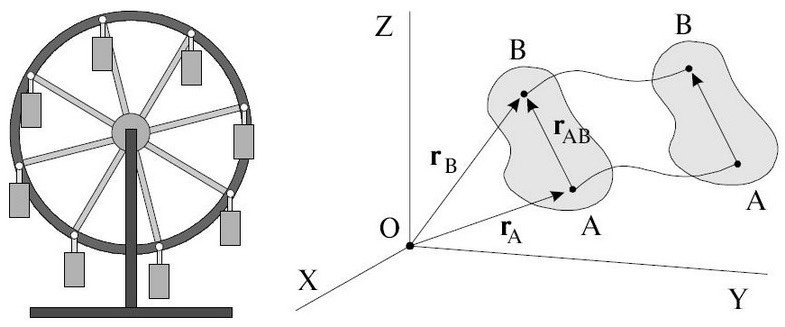
\includegraphics[width=8cm, height=3cm]{postup.jpg}
\end{center}
Траектории точек одинаковы, просто сдвиг на $r^\prime $, применим операцию дифференцирования к $r(t)$:
\[ \frac{dr}{dt} = \frac{dr_0}{dt} + \frac{dr^\prime}{dt} = 0 \Rightarrow v_M = v_A\]
Получаем что скорости точек А и М одинаковы, причем если мы еще раз продифференцируем это равенство получим что ускорения этих точек также равны.

\vspace{5px}

\textit{Для описания поступательного движения твердого тела достаточно описания движения лишь одной его точки.}


\subsection{Вращение твердого тела вокруг неподвижной оси}
Если при своем движении твердого тела 2 точки A и B не меняют своего положения, то говорят, что \textit{твердое тело вращается вокруг неподвижной оси}, проходящей через А и В, соответственно АВ - прямая являющаяся осью вращения.
\begin{center}
    \definecolor{fftttt}{rgb}{1,0.2,0.2}
    \definecolor{qqqqff}{rgb}{0,0,1}
    \definecolor{qqwuqq}{rgb}{0,0.39,0}
    \definecolor{qqqqcc}{rgb}{0,0,0.8}
    \begin{tikzpicture}[line cap=round,line join=round,>=triangle 45,x=1.0cm,y=1.0cm]
        \clip(7.98,22.58) rectangle (20.34,36.2);
        \draw [shift={(13,27)},color=qqwuqq,fill=qqwuqq,fill opacity=0.1] (0,0) -- (-143.13:0.6) arc (-143.13:-63.43:0.6) -- cycle;
        \draw [shift={(13,27)},line width=1.2pt,color=fftttt,fill=fftttt,fill opacity=0.1] (0,0) -- (71.57:1.2) arc (71.57:90:1.2) -- cycle;
        \draw [->] (13,27) -- (13,35);
        \draw [->] (13,27) -- (18,27);
        \draw [->] (13,27) -- (9,24);
        \draw [rotate around={100.82:(13.47,28.63)}] (13.47,28.63) ellipse (4.43cm and 1.96cm);
        \draw [->,color=qqqqcc] (13,27) -- (15,23);
        \draw [->,color=qqqqcc] (13,27) -- (17,32);
        \draw (15,23)-- (15,33);
        \draw (15,33)-- (13,34.11);
        \draw (13,34.11)-- (10,32.58);
        \draw (10,32.58)-- (10.03,24.77);
        \draw [rotate around={-0.63:(12.91,29.99)},dash pattern=on 3pt off 3pt] (12.91,29.99) ellipse (1.09cm and 0.6cm);
        \draw [->] (13,27) -- (14,30);
        \draw [->] (13.56,29.26) -- (14.4,30.6);
        \draw [dash pattern=on 3pt off 3pt] (14,30)-- (14,25);
        \draw (13.34,35.12) node[anchor=north west] {$z = z^\prime$};
        \draw (14,23.96) node[anchor=north west] {$x^\prime$};
        \draw (16.52,31.86) node[anchor=north west] {$y^\prime$};
        \draw (9.64,24.42) node[anchor=north west] {$x$};
        \draw (17.26,27.06) node[anchor=north west] {$y$};
        \draw (14,30)-- (13,30);
        \draw (13.36,30.62) node[anchor=north west] {$a$};
        \draw [shift={(13,27)},line width=1.2pt,color=fftttt] (71.57:1.2) arc (71.57:90:1.2);
        \draw [shift={(13,27)},line width=1.2pt,color=fftttt] (71.57:1.09) arc (71.57:90:1.09);
        \draw (14.28,30) node[anchor=north west] {$\vec w$};
        \draw (12.46,27.6) node[anchor=north west] {$O$};
        \begin{scriptsize}
            \fill [color=qqqqff] (14,30) circle (1.5pt);
            \fill [color=black] (13,30) circle (1.5pt);
            \draw[color=fftttt] (13.48,28.54) node {$\alpha$};
        \end{scriptsize}
    \end{tikzpicture}
\end{center}
Неподвижными точками будут и все точки на прямой АВ, то есть тело вращения имеет только одну степень свободы - достаточно лишь задать одну координату, чтобы определить положение тела в пространстве.

\vspace{5px}

$\phi(t) $ - функция определяющая положение тела в пространстве с помощью значения двухгранного угла, включающие отслеживаемую точку в разные моменты времени(причем траектория движения очевидно повторяет окружность)

\[ \alpha - const , a - const : a = r_M \cdot \sin{\alpha} \]
\[ \omega = \frac{d\phi}{dt} \]
\[ v = a \cdot \omega = r_M \cdot \sin{\alpha} \cdot \omega \] - причем вектор скорости будет направлен по оси вращения, формулы можем записать вектор скорости как $\vec v = [\omega, r] => \frac{dr}{dt} = [\omega,r]$. Так как $r - const$ такое равенство будет верно. Из этого выведем вектор ускорения:

\[ \vec w = \frac{dv}{dt} = \frac{d}{dt} [\vec \omega, \vec r] = [\frac{d\omega}{dt}, \vec r] + [\vec \omega, \frac{dr}{dt}] \] так как $\vec \omega$ - вектор, то и угловое ускорение $\vec \epsilon = \frac{d\omega}{dt}$ - вектор.

\vspace{5px}

Получаем :
\[ \vec w = \frac{d}{dt} [\vec \omega, \vec r] = [\frac{d\omega}{dt}, \vec r] + [\vec \omega, \frac{dr}{dt}] = [\vec \epsilon, \vec r] + [\vec \omega, \vec v]  = [\vec \epsilon, \vec r] + [\omega, [\omega,r]] \text{ ,где $ [\vec \epsilon, \vec r] = w_\tau $ , а  $[\omega, [\omega,r]] = w_n$}\]

\subsection{Скорость и ускорение точек абсолютно твердого тела при сложном движении}
\begin{center}
    \definecolor{fftttt}{rgb}{1,0.2,0.2}
    \definecolor{qqqqff}{rgb}{0,0,1}
    \definecolor{qqwuqq}{rgb}{0,0.39,0}
    \definecolor{qqqqcc}{rgb}{0,0,0.8}
    \begin{tikzpicture}[line cap=round,line join=round,>=triangle 45,x=1.4791176048705874cm,y=1.8441311417483108cm]
        \clip(44.96,95.72) rectangle (49.13,99.28);
        \draw [shift={(13,27)},color=qqwuqq,fill=qqwuqq,fill opacity=0.1] (0,0) -- (-143.13:0.27) arc (-143.13:-63.43:0.27) -- cycle;
        \draw [shift={(13,27)},line width=1.2pt,color=fftttt,fill=fftttt,fill opacity=0.1] (0,0) -- (71.57:0.53) arc (71.57:90:0.53) -- cycle;
        \draw [->] (13,27) -- (13,35);
        \draw [->] (13,27) -- (18,27);
        \draw [->] (13,27) -- (9,24);
        \draw [rotate around={100.82:(13.47,28.63)}] (13.47,28.63) ellipse (6.55cm and 3.61cm);
        \draw [->,color=qqqqcc] (13,27) -- (15,23);
        \draw [->,color=qqqqcc] (13,27) -- (17,32);
        \draw (15,23)-- (15,33);
        \draw (15,33)-- (13,34.11);
        \draw (13,34.11)-- (10,32.58);
        \draw (10,32.58)-- (10.03,24.77);
        \draw [rotate around={-0.63:(12.91,29.99)},dash pattern=on 1pt off 1pt] (12.91,29.99) ellipse (1.61cm and 1.11cm);
        \draw [->] (13,27) -- (14,30);
        \draw [->] (13.56,29.26) -- (14.4,30.6);
        \draw [dash pattern=on 1pt off 1pt] (14,30)-- (14,25);
        \draw (13.34,34.99) node[anchor=north west] {$z = z^\prime$};
        \draw (14,23.83) node[anchor=north west] {$x^\prime$};
        \draw (16.52,31.73) node[anchor=north west] {$y^\prime$};
        \draw (9.64,24.29) node[anchor=north west] {$x$};
        \draw (17.26,26.92) node[anchor=north west] {$y$};
        \draw (14,30)-- (13,30);
        \draw (13.36,30.49) node[anchor=north west] {$a$};
        \draw [shift={(13,27)},line width=1.2pt,color=fftttt] (71.57:0.53) arc (71.57:90:0.53);
        \draw [shift={(13,27)},line width=1.2pt,color=fftttt] (71.57:0.48) arc (71.57:90:0.48);
        \draw (14.28,29.87) node[anchor=north west] {$\vec w$};
        \draw (12.46,27.46) node[anchor=north west] {$O$};
        \draw [->] (46,96.5) -- (46,99);
        \draw [->] (46,96.5) -- (45.5,96);
        \draw [->] (46,96.5) -- (48.5,96.5);
        \draw [rotate around={-8.45:(47.48,97.43)},fill=black,fill opacity=0.1] (47.48,97.43) ellipse (1.79cm and 0.96cm);
        \draw [->] (46,96.5) -- (47,97.5);
        \draw [->] (47,97.5) -- (47.01,98.59);
        \draw [->] (47,97.5) -- (48,97.5);
        \draw [->] (46,96.5) -- (48,97.5);
        \draw (46.65,98.29) node[anchor=north west] {$\vec w$};
        \draw (46.69,97.84) node[anchor=north west] {$A$};
        \draw (47.37,97.9) node[anchor=north west] {$\vec a$};
        \draw (46.25,97.4) node[anchor=north west] {$\vec r_0$};
        \draw (47.06,96.97) node[anchor=north west] {$\vec r$};
        \draw (45.59,96.95) node[anchor=north west] {$O$};
        \draw (45.29,96.51) node[anchor=north west] {$x$};
        \draw (45.67,99.17) node[anchor=north west] {$z$};
        \draw (48.26,96.46) node[anchor=north west] {$y$};
        \draw (47.87,97.82) node[anchor=north west] {$M$};
        \begin{scriptsize}
            \fill [color=qqqqff] (14,30) circle (1.5pt);
            \fill [color=black] (13,30) circle (1.5pt);
            \draw[color=fftttt] (44.31,102.25) node {$\alpha$};
            \fill [color=black] (47,97.5) circle (1.5pt);
            \fill [color=black] (48,97.5) circle (1.5pt);
        \end{scriptsize}
    \end{tikzpicture}
\end{center}
Пусть M - произвольная точка твердого тела.
\[\vec r = \vec r_0 +\vec a , |\vec a| = const\]
\begin{flushright}
    -берем модуль поскольку может меняться направление движения (произвольное движение)
\end{flushright}
Продифференцируем по t
\[\vec v_M = \vec v_A + \frac{d\vec a}{dt} \text{ ,где $\frac{d\vec a}{dt} = [\vec \omega, \vec a]$(из вращательного движения)}\]
Тогда:
\[\vec v_m = \vec v_A + [\vec w, \vec a]\]

$\vec v_A$ - скорость поступательного движения

$[\vec w, \vec a]$ - вращательное движение вокруг подвижной оси

Еще раз продифференцируем по t
\[\vec w_M = \vec w_a + \frac{d[\vec w, \vec a]}{dt}\]
\[\vec w_M = \vec w_A + [\vec \epsilon, \vec a] + [\vec w, [\vec w, \vec a]]\]
где $\vec w_A$ - поступательное ускорение, а $[\vec \epsilon, \vec a] + [\vec w, [\vec w, \vec a]]$ - ускорение вращательного движения

\subsection{Инвариантность вектора угловой скорости}
Инвариантность вектора угловой скорости означает, что вектор угловой скорости сохраняет свое направление и величину в инерциальной системе отсчета, независимо от движения самого тела. Другими словами, если тело вращается относительно неподвижной точки его угловая скорость будет одинаковой в любой инерциальной системе отсчета.
\begin{center}
    \definecolor{xdxdff}{rgb}{0.49,0.49,1}
    \definecolor{qqqqff}{rgb}{0,0,1}
    \begin{tikzpicture}[line cap=round,line join=round,>=triangle 45,x=1.5539478252200503cm,y=1.598362350181992cm]
        \clip(12.73,23.91) rectangle (16.34,27.26);
        \draw [->] (14,12.57) -- (14,15.5);
        \draw [->] (13.5,13) -- (17,13);
        \draw [shift={(16.15,15.15)}] plot[domain=3.23:4.62,variable=\t]({1*1.66*cos(\t r)+0*1.66*sin(\t r)},{0*1.66*cos(\t r)+1*1.66*sin(\t r)});
        \draw (14,15)-- (14.5,15);
        \draw (14.5,15)-- (14.5,13);
        \draw (16,14.5)-- (14,14.5);
        \draw (16,14.5)-- (16,13);
        \draw [rotate around={-54.68:(14.56,25.5)}] (14.56,25.5) ellipse (2.43cm and 1.85cm);
        \draw [->] (14,26) -- (15,26);
        \draw [->] (14.5,25) -- (15,26);
        \draw [->] (14,26) -- (14.5,25);
        \draw (14.34,26.43) node[anchor=north west] {$\vec a$};
        \draw (14.84,25.73) node[anchor=north west] {$\vec b$};
        \draw (13.96,25.64) node[anchor=north west] {$\vec r$};
        \draw (13.69,26.35) node[anchor=north west] {$A$};
        \draw (15.01,26.29) node[anchor=north west] {$M$};
        \draw (14.52,25.07) node[anchor=north west] {$B$};
        \begin{scriptsize}
            \fill [color=qqqqff] (14,12.57) circle (1.5pt);
            \draw[color=qqqqff] (12.62,28.84) node {$A$};
            \fill [color=qqqqff] (14,15.5) circle (1.5pt);
            \draw[color=qqqqff] (12.62,28.84) node {$B$};
            \fill [color=qqqqff] (13.5,13) circle (1.5pt);
            \draw[color=qqqqff] (12.62,28.84) node {$C$};
            \fill [color=qqqqff] (17,13) circle (1.5pt);
            \draw[color=qqqqff] (12.62,28.84) node {$D$};
            \fill [color=qqqqff] (14.5,15) circle (1.5pt);
            \draw[color=qqqqff] (12.61,28.84) node {$E$};
            \fill [color=qqqqff] (14.91,14.06) circle (1.5pt);
            \draw[color=qqqqff] (12.61,28.84) node {$F$};
            \fill [color=qqqqff] (16,13.5) circle (1.5pt);
            \draw[color=qqqqff] (12.62,28.84) node {$G$};
            \fill [color=xdxdff] (14,15) circle (1.5pt);
            \draw[color=xdxdff] (12.62,28.84) node {$H$};
            \fill [color=xdxdff] (14.5,13) circle (1.5pt);
            \draw[color=xdxdff] (12.6,28.84) node {$I$};
            \fill [color=qqqqff] (16,14.5) circle (1.5pt);
            \draw[color=qqqqff] (12.6,28.84) node {$J$};
            \fill [color=qqqqff] (14,14.5) circle (1.5pt);
            \draw[color=qqqqff] (12.61,28.84) node {$K$};
            \fill [color=xdxdff] (16,13) circle (1.5pt);
            \draw[color=xdxdff] (12.61,28.84) node {$L$};
        \end{scriptsize}
    \end{tikzpicture}
\end{center}


\[ \vec v_M = \vec v_A + [\omega, a]\]
\[\vec v_B = v_A + [\vec \omega, \vec r]\]
\[ \vec v_M = \vec v_B + [\vec \omega, b]\]
\[ v_M = \vec v_A + [w, r+b] = v_A + [\omega, r] + [\omega, b] = v_B + [\omega, b]\]

\textit{Вывод: $\vec \omega = \vec \omega^\prime $, то есть угловая скорость не зависит от выбора полюса. И тогда возникает вопрос: как найти наиболее оптимальный полюс?}

\vspace{10px}

\textbf{Ситуация 1:} \[ \vec \omega \perp v_A\]
\begin{center}
    \begin{tikzpicture}[line cap=round,line join=round,>=triangle 45,x=2.244876513087598cm,y=2.2255761020319826cm]
        \clip(16.91,15.65) rectangle (21.73,18.1);
        \draw [rotate around={3.89:(19.23,16.61)},fill=black,fill opacity=0.1] (19.23,16.61) ellipse (3.65cm and 1.18cm);
        \draw [->] (18.49,16.76) -- (18.5,18);
        \draw [->] (18.49,16.76) -- (20.51,16.76);
        \draw [->] (18.49,16.76) -- (19.18,16.24);
        \draw [->] (18.49,16.76) -- (20,16.5);
        \draw [->] (19.18,16.24) -- (20,16.5);
        \draw (18.03,17.59) node[anchor=north west] {$\vec \omega$};
        \draw (20.19,17.11) node[anchor=north west] {$\vec v_A$};
        \draw (18.67,17.1) node[anchor=north west] {$A$};
        \draw (18.62,16.58) node[anchor=north west] {$\vec r$};
        \draw (19.74,16.86) node[anchor=north west] {$\vec a$};
        \draw (19.69,16.49) node[anchor=north west] {$\vec b$};
        \draw (20.09,16.69) node[anchor=north west] {$M$};
        \draw (18.92,16.38) node[anchor=north west] {$O$};
        \begin{scriptsize}
            \fill [color=black] (18.49,16.76) circle (1.5pt);
            \fill [color=black] (20,16.5) circle (1.5pt);
        \end{scriptsize}
    \end{tikzpicture}
\end{center}
\[v_M = v_0 + [\omega,\vec b] \]
\[\vec v_0 = \vec v_A + [\vec \omega, \vec r]\]

Выбираем r  так, чтобы $[w,r] = -v_A$, то есть
\[ v_0 = \vec v_A - \vec v_A = 0 \]

Получаем \[ v_M = [\omega, b]\] - есть только вращательная составляющая скорости, причем ось OM называют мнимой осью.

\vspace{8px}

\textbf{Ситуация 2:} $\vec \omega$ не перпендикулярно $v_A$ , так тогда можем разложить $v_A$ на ортогональную проекцию и ортогональную составляющую. Тогда применим ситуацию 1 и получим что:
$[\omega,r] = -v_A$(ортогональная проекция), а соответственно ортогональная составляющая будет перпендикулярна $\omega$.

Тогда : \[ v_M = v_A + [\omega, b] \text{--- винтовое движение} \]

\chapter{Динамика}
\section{Динамика материальной точки. Законы Ньютона}
\subsection{Первый закон Ньютона}
\textit{\textbf{Первый закон Ньютона :} Существует такая система отсчета в которой всякое тело покоится или прямолинейно и равномерно движется до тех пор пока воздействие со стороны других тел не изменяет этого состояния - инерциальные системы отсчета (ИСО).}

\vspace{5px}

В ИСО пространство однородно и изотропно, а время однородно.
\begin{itemize}
    \item \textit{Однородность} пространства означает, что во всех его точках все физические законы действуют одинаково.
    \item \textit{Изотропность} пространства означает, что по всем направлениям пространства все физические законы(на вектора) действуют одинаково
    \item О\textit{днородность времени} означает, что во все моменты времени все физические законы действуют одинаково.
\end{itemize}
\textit{Любая система отсчета, которая покоиться или движется прямолинейно и равномерно относительно инерциальной тоже будет ИСО, следовательно их бесконечное множество}
\subsection{Понятие силы и массы.Второй закон Ньютона}

--- \textbf{Определение: \textit{Масса}} - мера инертности тела. Под инертностью понимают способность тела сопротивляться внешнему воздействию.

\vspace{5px}

--- \textbf{Определение: \textit{Сила}} - мера взаимодействия тел. Она может проявляться либо в получении ускорения, либо в деформации.

\begin{enumerate}
    \item \textbf{\textit{Принцип независимого действия }}

          Действия силы на тело не зависит от того покоится это тело или движется, а также не зависит от количества и вида других сил, действующих на это тело.
          \newpage
    \item \textbf{\textit{Принцип суперпозиции тел}}

          \textbf{Определение:} Если на тело действует несколько сил, то их совместное действие можно заменить действию одной силы, равной векторной сумме сил. Такую силу называют равнодействующей силой.

          Если на тело действует система сил, равнодействующая который равна $\vec 0$, то тело не меняет своё состояние.
\end{enumerate}
\textit{\textbf{Второй закон Ньютона:} ускорение тела прямо пропорционально силе, действующей на тело и обратно пропорционально массе тела} \[ \vec w = k \cdot \frac{\vec F}{m} \] где $\vec F$ - равнодействующая сила, k - коэффициент пропорциональности из-за разных единиц измерения w, m, F
\[ \vec F = m \cdot \vec W\]

Выберем единицы измерения так, чтобы k = 1, получаем:
\[[F] = \frac{\text{кг}\cdot\text{м}}{c^2} = \text{Н}\]

\textit{\textbf{Третий закон Ньютона:} действие тел друг на друга носит характер взаимодействия. Силы, с которыми тела действуют друг на друга равны по величине, но противоположны по направлению.}
\[\vec F_{12} = - \vec F_{21}\]

$\vec F_{12}$ - сила, действующая на второе тело от первого, $\vec F_{21}$ -сила, действующая на первое тело от второго
\subsection{Принцип относительности Галилея}
\begin{center}
    \begin{tikzpicture}[line cap=round,line join=round,>=triangle 45,x=0.5921540164917828cm,y=0.507076355328508cm]
        \clip(11.89,17.64) rectangle (24.15,29.81);
        \draw [->] (16,20) -- (16,28);
        \draw [->] (16,20) -- (22,20);
        \draw [->] (16,20) -- (12,18);
        \draw [->] (18,26) -- (17.97,23.35);
        \draw [->] (18,26) -- (21.65,26.02);
        \draw [->] (18,26) -- (20.86,29.4);
        \draw [->] (18,26) -- (20.37,27.18);
        \draw [->] (16,20) -- (18,26);
        \draw [->] (18,26) -- (20,20);
        \draw (16.39,24.7) node[anchor=north west] {$\vec r_0$};
        \draw (19.31,23.84) node[anchor=north west] {$\vec r^\prime$};
        \draw (15.26,21.4) node[anchor=north west] {$O$};
        \draw (17.61,27.48) node[anchor=north west] {$O^\prime$};
        \draw (20.4,29.93) node[anchor=north west] {$z^\prime$};
        \draw (19.7,29.93) node[anchor=north west] {$z^\prime$};
        \draw (20.98,27.37) node[anchor=north west] {$x^\prime$};
        \draw (17.88,23.73) node[anchor=north west] {$y^\prime$};
        \draw (20.16,28.69) node[anchor=north west] {$\vec v_0$};
        \draw (20.22,19.78) node[anchor=north west] {$M$};
        \begin{scriptsize}
            \fill [color=black] (16,20) circle (1.5pt);
            \fill [color=black] (18,26) circle (1.5pt);
            \fill [color=black] (20,20) circle (1.5pt);
        \end{scriptsize}
    \end{tikzpicture}
\end{center}

Возьмем две инерциальные системы отсчета. Пусть $\vec v_0$ - постоянный вектор, $O x^\prime y^\prime z^\prime$ - подвижная система (движется прямолинейно и равномерно)
\[ \vec r = \vec r^\prime + \vec r_0 \Rightarrow \]
\[ \vec v = \vec v^\prime + \vec v_0(const) \Rightarrow \]
\[ \vec w = \vec w^\prime \]
\textit{\textbf{Принцип относительности Галилея:} Так как и масса и ускорение точки М равны в обеих системах отсчета, то во всех инерциальных системах отсчета силы действуют одинаково.}

\vspace{5px}

\textbf{Следствие:} Никакими опытами невозможно определить движется ли наша (инерциальная) система отсчета прямолинейно и равномерно или не движется.

\section{Виды сил}
\begin{enumerate}
    \item \underline{Сила тяжести.}
          \begin{center}
              \begin{tikzpicture}[line cap=round,line join=round,>=triangle 45,x=1.0cm,y=1.0cm]
                  \clip(5.33,10.9) rectangle (15.43,15.81);
                  \fill[fill=black,fill opacity=0.1] (6,13) -- (6,12) -- (11,12) -- (11,13) -- cycle;
                  \fill[fill=black,fill opacity=0.1] (12.46,12) -- (13.38,12) -- (13.38,12.98) -- (12.48,12.98) -- cycle;
                  \draw (8,13)-- (8,14);
                  \draw (8,14)-- (9,14);
                  \draw (9,14)-- (9,13);
                  \draw (9,13)-- (8,13);
                  \draw (6,13)-- (11,13);
                  \draw [->] (8.46,13.56) -- (8.46,12.14);
                  \draw [->] (8.66,13) -- (8.66,11.74);
                  \draw (6,13)-- (6,12);
                  \draw (6,12)-- (11,12);
                  \draw (11,12)-- (11,13);
                  \draw (11,13)-- (6,13);
                  \draw (7.86,12.97) node[anchor=north west] {$G$};
                  \draw (8.78,12.84) node[anchor=north west] {$p$};
                  \draw (12,12)-- (12,15);
                  \draw (12,15)-- (14,15);
                  \draw (14,15)-- (14,12);
                  \draw (14,12)-- (12,12);
                  \draw (12.46,12)-- (13.38,12);
                  \draw (13.38,12)-- (13.38,12.98);
                  \draw (13.38,12.98)-- (12.48,12.98);
                  \draw (12.48,12.98)-- (12.46,12);
                  \draw [->] (12.84,12.56) -- (12.84,11.32);
                  \draw [->] (13,12) -- (13.01,11.08);
                  \draw [->] (13.19,12) -- (13.21,13.96);
                  \draw (13.29,13.89) node[anchor=north west] {$\bar N$};
                  \draw (13.07,11.97) node[anchor=north west] {$p$};
                  \draw (12.22,12.06) node[anchor=north west] {$G $};
                  \begin{scriptsize}
                      \fill [color=black] (8.46,13.56) circle (1.5pt);
                      \fill [color=black] (12.84,12.56) circle (1.5pt);
                  \end{scriptsize}
              \end{tikzpicture}
              \label{tikz_example}
          \end{center}

          \textbf{Определение: \textit{Сила тяжести $[G]$}}- сила притяжения Земли, действующая на материальные объекты вблизи ее поверхности, $G = m \cdot g$. Сила тяжести приложена к телу.

          \textbf{Определение: \textit{Вес $[p]$}} - сила, с которой тело действует на опору или подвес. Вес приложен к опоре.

          Причем важно сказать, что вес и сила тяжести равны только для тел находящихся в покое.

          \textbf{Определение: \textit{Сила нормального давления $[\vec N]$}} - сила, с которой опора действует на тело, так $|\bar N| = | p |$ из третьего закона Ньютона.

          \vspace{5px}

          Рассмотрим движение лифта на рисунке \ref{tikz_example}:
          \begin{enumerate}
              \item \textit{вектор ускорения направлен вверх, $\uparrow a, |a| \textless g$}
                    (рисунок выше)

                    \vspace{5px}

                    Применим второй закон Ньютона, а именно: $m \cdot -a = mg + N \langle |N| = |p| \rangle = mg + p$, отсюда $p = m \cdot (g+a) \textgreater G $
              \item \textit{вектор ускорения направлен вниз, $\downarrow a, |a| \textless g$}

                    \vspace{5px}

                    Применим второй закон Ньютона, а именно: $m \cdot a = mg + N \langle |N| = |p| \rangle = mg + p$, отсюда $p = m \cdot (g-a) \textless G $
              \item \textit{вектор ускорения направлен вверх, $\uparrow a, |a| \textgreater g$}
                    Тогда измениться лишь то, что тело будет действовать на другую опору, а именно на грань $O_1$

                    \vspace{5px}

              \item \textit{$|a| = g$, то есть лифт находится в состоянии свободного падения. }

                    \vspace{5px}

                    Тогда по формулам получим, что $|N| = 0 = |p|$,то есть тело будет находится в невесомости.
              \item \textit{Рассмотрим движение по окружности, так чтобы тело оставалось на одной высоте(пример: движение спутника по орбите)}

                    \vspace{5px}

                    Тогда $w_n = g = \frac{v^2}{R_3}$
          \end{enumerate}

    \item \underline{Сила упругости(рассматриваем такие деформации как растяжение, стяжения)}

          \textit{\textbf{Закон Гука} : деформация, возникающая в упругом теле, пропорциональна приложенной к этому телу силе.}

          $\vec F = -k \cdot \Delta x$
    \item \underline{Сила трения}

          Есть 2 разделения этой силы на типы.

          I. \begin{itemize}
              \item внешние
              \item внутренние
          \end{itemize}

          II. \begin{itemize}
              \item \textbf{Определение:} Силы сухого трения - силы возникающие при трении двух твердых тел
                    \begin{enumerate}
                        \item сила трения покоя: $|F_{tr}| = |F|, F_{tr} = -F$
                              \begin{center}
                                  \begin{tikzpicture}[line cap=round,line join=round,>=triangle 45,x=0.5388319470138785cm,y=0.5075527225504726cm]
                                      \clip(9.79,48.46) rectangle (20.64,52.53);
                                      \fill[fill=black,fill opacity=0.1] (6,13) -- (6,12) -- (11,12) -- (11,13) -- cycle;
                                      \fill[fill=black,fill opacity=0.1] (12.46,12) -- (13.38,12) -- (13.38,12.98) -- (12.48,12.98) -- cycle;
                                      \fill[fill=black,fill opacity=0.1] (10,50) -- (20,50) -- (19.94,48.76) -- (9.95,48.73) -- cycle;
                                      \draw (8,13)-- (8,14);
                                      \draw (8,14)-- (9,14);
                                      \draw (9,14)-- (9,13);
                                      \draw (9,13)-- (8,13);
                                      \draw [->] (8.46,13.56) -- (8.46,12.14);
                                      \draw [->] (8.66,13) -- (8.66,11.74);
                                      \draw (6,13)-- (6,12);
                                      \draw (6,12)-- (11,12);
                                      \draw (11,12)-- (11,13);
                                      \draw (11,13)-- (6,13);
                                      \draw (7.85,13.11) node[anchor=north west] {$G$};
                                      \draw (8.8,12.97) node[anchor=north west] {$p$};
                                      \draw (12,12)-- (12,15);
                                      \draw (12,15)-- (14,15);
                                      \draw (14,15)-- (14,12);
                                      \draw (14,12)-- (12,12);
                                      \draw (12.46,12)-- (13.38,12);
                                      \draw (13.38,12)-- (13.38,12.98);
                                      \draw (13.38,12.98)-- (12.48,12.98);
                                      \draw (12.48,12.98)-- (12.46,12);
                                      \draw [->] (12.84,12.56) -- (12.84,11.32);
                                      \draw [->] (13,12) -- (13.01,11.08);
                                      \draw [->] (13.19,12) -- (13.21,13.96);
                                      \draw (13.29,14.03) node[anchor=north west] {$\bar N$};
                                      \draw (13.08,12.09) node[anchor=north west] {$p$};
                                      \draw (12.23,12.19) node[anchor=north west] {$G $};
                                      \draw (10,50)-- (20,50);
                                      \draw (14,50)-- (14,52);
                                      \draw (14,52)-- (16,52);
                                      \draw (16,52)-- (16,50);
                                      \draw (16,50)-- (14,50);
                                      \draw [->] (15.03,51.06) -- (19.97,51.06);
                                      \draw [->] (15.03,51.06) -- (11.46,51.1);
                                      \draw (12.51,52.56) node[anchor=north west] {$\vec F_{tr}$};
                                      \draw (16.96,52.63) node[anchor=north west] {$\vec F$};
                                      \begin{scriptsize}
                                          \fill [color=black] (8.46,13.56) circle (1.5pt);
                                          \fill [color=black] (12.84,12.56) circle (1.5pt);
                                          \fill [color=black] (15.03,51.06) circle (1.5pt);
                                          \draw[color=black] (15.51,51.5) node {$L_1$};
                                      \end{scriptsize}
                                  \end{tikzpicture}
                              \end{center}

                        \item сила трения скольжения $F = \mu \cdot N$
                              \begin{center}
                                  \begin{tikzpicture}[line cap=round,line join=round,>=triangle 45,x=0.424582259472394cm,y=0.3904081721537406cm]
                                      \clip(9.45,48.06) rectangle (33.78,56.26);
                                      \fill[fill=black,fill opacity=0.1] (6,13) -- (6,12) -- (11,12) -- (11,13) -- cycle;
                                      \fill[fill=black,fill opacity=0.1] (12.46,12) -- (13.38,12) -- (13.38,12.98) -- (12.48,12.98) -- cycle;
                                      \fill[fill=black,fill opacity=0.1] (10,50) -- (20,50) -- (19.94,48.76) -- (9.95,48.73) -- cycle;
                                      \draw (8,13)-- (8,14);
                                      \draw (8,14)-- (9,14);
                                      \draw (9,14)-- (9,13);
                                      \draw (9,13)-- (8,13);
                                      \draw [->] (8.46,13.56) -- (8.46,12.14);
                                      \draw [->] (8.66,13) -- (8.66,11.74);
                                      \draw (6,13)-- (6,12);
                                      \draw (6,12)-- (11,12);
                                      \draw (11,12)-- (11,13);
                                      \draw (11,13)-- (6,13);
                                      \draw (7.84,13.23) node[anchor=north west] {$G$};
                                      \draw (8.81,13.09) node[anchor=north west] {$p$};
                                      \draw (12,12)-- (12,15);
                                      \draw (12,15)-- (14,15);
                                      \draw (14,15)-- (14,12);
                                      \draw (14,12)-- (12,12);
                                      \draw (12.46,12)-- (13.38,12);
                                      \draw (13.38,12)-- (13.38,12.98);
                                      \draw (13.38,12.98)-- (12.48,12.98);
                                      \draw (12.48,12.98)-- (12.46,12);
                                      \draw [->] (12.84,12.56) -- (12.84,11.32);
                                      \draw [->] (13,12) -- (13.01,11.08);
                                      \draw [->] (13.19,12) -- (13.21,13.96);
                                      \draw (13.28,14.15) node[anchor=north west] {$\bar N$};
                                      \draw (13.05,12.21) node[anchor=north west] {$p$};
                                      \draw (12.22,12.3) node[anchor=north west] {$G $};
                                      \draw (10,50)-- (20,50);
                                      \draw (14,50)-- (14,52);
                                      \draw (14,52)-- (16,52);
                                      \draw (16,52)-- (16,50);
                                      \draw (16,50)-- (14,50);
                                      \draw [->] (15.03,51.06) -- (19.97,51.06);
                                      \draw [->] (15.03,51.06) -- (11.46,51.1);
                                      \draw (11.99,52.95) node[anchor=north west] {$\vec F_{tr}$};
                                      \draw (16.6,52.81) node[anchor=north west] {$\vec F = \mu \cdot \bar N$};
                                      \draw [->] (26,48) -- (26,56);
                                      \draw [->] (22,52) -- (32,52);
                                      \draw [dash pattern=on 1pt off 1pt] (26,54)-- (20,54);
                                      \draw [dash pattern=on 1pt off 1pt] (26,50)-- (32,50);
                                      \draw [shift={(22.81,57.34)}] plot[domain=3.91:5.65,variable=\t]({1*3.95*cos(\t r)+0*3.95*sin(\t r)},{0*3.95*cos(\t r)+1*3.95*sin(\t r)});
                                      \draw [shift={(29.08,46.67)}] plot[domain=0.74:2.46,variable=\t]({1*3.95*cos(\t r)+0*3.95*sin(\t r)},{0*3.95*cos(\t r)+1*3.95*sin(\t r)});
                                      \draw (26.23,56.17) node[anchor=north west] {$F_{tr}$};
                                      \draw (31.3,52.21) node[anchor=north west] {$v$};
                                      \draw (26.32,54.79) node[anchor=north west] {$\mu$};
                                      \draw (24.06,50.87) node[anchor=north west] {$- \mu$};
                                      \draw (15.4,54.33) node[anchor=north west] {$\vec v$};
                                      \draw [->] (15.55,52.69) -- (16.2,52.69);
                                      \begin{scriptsize}
                                          \fill [color=black] (8.46,13.56) circle (1.5pt);
                                          \fill [color=black] (12.84,12.56) circle (1.5pt);
                                          \fill [color=black] (15.03,51.06) circle (1.5pt);
                                      \end{scriptsize}
                                  \end{tikzpicture}
                              \end{center}
                        \item сила трения качения:
                    \end{enumerate}
              \item \textbf{Определение:} Силы вязкого трения - силы, возникающие при трении твердого тела в жидкой, газообразной среде, между слоями тел.

                    \vspace{5px}

                    Рассмотрим движение в жидком вторнике, так:
                    \[ \vec F =  - \alpha_1 \cdot \vec v \text{--- сопротивление при небольшой скорости(для каждого четверга разная)}\]
                    \[ \vec F =  - \alpha_2 \cdot \vec v \cdot v \text{--- сопротивление при большой скорости.}\]
          \end{itemize}
\end{enumerate}
\section{Примеры интегрирования уравнения движения для материальных точек}

Основное уравнение движения материальной точки задается вторым законом Ньютона, а именно \[ m \cdot \frac{d\vec v}{dt} = \vec F\] с начальными условиями: \[ v(0) = v_0, r(0) = r_0\]

\begin{enumerate}
    \item Сила зависит от \textit{времени}

          \[
              \begin{cases}
                  m \cdot \frac{d\vec v}{dt} = \vec F(t) \\
                  \vec v = (v_x, v_y, v_z)               \\
                  \vec r = (x,y,z)                       \\
                  \vec F = (F_x, F_y, F_z)
              \end{cases}
          \]
          \[
              \begin{cases}
                  m \cdot \frac{dv_x}{dt} = F_x(t) \\
                  m \cdot \frac{dv_y}{dt} = F_y(t) \\
                  m \cdot \frac{dv_z}{dt} = F_z(t)
              \end{cases}
          \]
          Рассмотрим для $v_x(0) = v_{x_0} ; x(0) = x_0 $, для остальных аналогично:
          \[ dv_x = \frac{1}{m} \cdot F_x(t) dt\]
          \[\int_{v_{x0}}^{v_x} \,du = \frac{1}{m} \cdot \int_{0}^{t} F_x(\xi) \,d\xi \]
          \[v_x = v_{x_0} + \frac{1}{m} \cdot \int_{0}^{t} F_x(\xi) \,d\xi\]
          \[\frac{dx}{dt} = v_x \Rightarrow \int \,dx = \int v_x \,dx \]
          \[x = x_0 + v_{x_0}t + \int_{0}^{t}  (\int_{0}^{\eta} F_x(\xi) \,d\xi) \,d\eta \]
    \item Координаты вектора силы зависят от соответствующих \textit{координат скорости}
          \[
              \begin{cases}
                  \vec m \cdot \frac{dv_x}{dt} = \vec F_x(v_x) \\
                  v = (v_x, v_y, v_z)                          \\
                  \vec r = (x,y,z)                             \\
                  \vec F = (F_x(v_x), F_y(v_y), F_z(v_z))
              \end{cases}
          \]
          Рассмотрим для $v_x(0) = v_{x_0} ; x(0) = x_0$:
          \[\frac{dv_x}{F_x(v_x)} = \frac{dt}{m}\]
          \[\frac{t}{m} = \int_{v_{x_0}}^{v_x} \frac{du}{F_x(u)}\] --- отсюда получаем зависимости времени то скорости, а именно $t = \phi(v_x) => v_x = \phi^{-1}(t)$, пользуясь этим соотношением получим:
          \[\frac{dx}{dt} = \phi^{-1}(t), x(0) = x_0\]
          \[x = x_0 + \int_{0}^{t} \phi^{-1}(\tau) \,d\tau \]
          Подставим:
          \[ \frac{dx}{dt} = v_x \Rightarrow dt = \frac{dx}{v_x} \]
          \[ \frac{m \cdot v_xdv_x}{dx} = F_x(v_x), v(x_0) = v_{x0} \]
          \[ \frac{m \cdot v_xdv_x}{F_x(v_x)} = dx\]
          \[x = x_0 + \int_{v_{x_0}}^{v_x} \frac{m \cdot udu}{F_x(u)} \]
    \item Координаты вектора силы зависят от соответствующих \textit{координат радиус-вектора $\vec r$}
          \[
              \begin{cases}
                  \vec m \cdot \frac{dv_x}{dt} = \vec F_x(x) \\
                  v = (v_x, v_y, v_z)                        \\
                  \vec r = (x,y,z)                           \\
                  \vec F = (F_x(x), F_y(y), F_z(z))
              \end{cases}
          \]
          \[m \cdot \frac{d^2x}{dt} = F_x(x) \text{, где} \frac{dx}{dt} = v_x \Rightarrow dt = \frac{dx}{v_x}\]
          Подставим:

          \[m\cdot \frac{v_xdv_x}{dx} = F_x(x)\]
          \[dv_x^2 = \frac{2}{m} F_x(x)dx , v_x(x_0) = v_{x0}\]
          \[ v_x = \sqrt{\frac{2}{m} \cdot \int_{x_0}^{x}F(\xi)d\xi + v_{x0}^2}\]
          --- знак может быть определен из начального условия $v_x(0) = v_{x0}$
          \[\frac{dx}{dt} = \phi(x), x(0) = x_0 \Rightarrow \]
          \[\frac{dx}{\phi(x)} = dt, t = \int_{x_0}^{x}\phi(\xi) \,d\xi\]
    \item Сила есть сумма \textit{сил(с силами трения)}
          \[ \vec F = \vec F_1(t) - \mu \vec v - k\vec r\]
          В одномерном случае
          \[m \cdot \frac{dv}{dt} = F_1(t) - \mu v - kx , v(0) = v_0, x(0) = x_0\]
          \[m \cdot \frac{d^2x}{dt^2} = F_1(t) - \mu \frac{dx}{dt} - kx \]
          Поделим на m и введем новые обозначения:
          \[ \alpha = \frac{\mu}{m}, \omega^2 = \frac{k}{m}, f = \frac{F}{m} \]
          Тогда, с учетом замены выше, получим
          \[\ddot x + \alpha \dot x + \omega^2x = f(t), v(0) = v_0, x(0) = x_0\]
\end{enumerate}
\section{Динамические характеристики движения}
\[ m \cdot \vec w = \vec F \]
\[ \frac{d(m \cdot \vec v)}{dt} = \vec F\]
где $m\vec v = \vec p$ - импульс точки - физическая величина, характеризующая движение материальной точки.

Получим:
\[ \frac{d\vec p}{dt} = \vec F => d\vec p = \vec F dt\]
где $\vec Fdt$ - элементарный импульс силы. Проинтегрируем $p(t_1) = p_1, p(t_2) = p_2$ от $p_1$ до $p_2$:
\[ \int_{p_1}^{p_2}\,d\vec p  = \int_{t_1}^{t_2} \vec F \,dt \]
\[\vec p_2 - \vec p_1 = \Delta \vec p = \int_{t_1}^{t_2} \vec F \,dt\]
--- \textbf{\textit{интегральная форма записи второго закона Ньютона}}, где $\int_{t_1}^{t_2} \vec F \,dt$ - импульс силы за промежуток времени.

\vspace{5px}

--- \textbf{Определение:} Моментом вектора $\vec a$ относительно точки О называется векторное произведение $[\vec r, \vec a]; mom_O \vec a = [\vec r, \vec a]$.

\vspace{5px}

--- \textbf{Определение:} Момент импульса $\vec L = [\vec r, \vec p]$

\vspace{5px}

--- \textbf{Определение:} Момент силы $\vec M = [\vec r, \vec F]$

\vspace{5px}

Рассмотрим $\frac{d\vec p}{dt} = \vec F$, умножим векторно слева на $\vec r$:
\[ [\vec r, \frac{d \vec p}{dt}] = [\vec r, \vec F]\]
Рассмотрим $\frac{d\vec L}{dt}$:
\[\frac{d\vec L}{dt} = \frac{d}{dt}[\vec r, \vec p] = [\frac{d\vec r}{dt}, \vec p] + [\vec r, \frac{d \vec p}{dt}] = [\vec v, m \vec v] + [\vec r, \frac{d\vec p}{dt}] = \vec 0 + [\vec r, \frac{d\vec p}{dt}] = \vec M\]

\section{Работа}
\subsection{Работа}
Пусть точка перемещается под действием силы $\vec F$.Ее элементарное перемещение есть $d\vec r$($\vec F$ и $d\vec r$ не обязательно сонаправленны)

\vspace{3px}

--- \textbf{Определение: \textit{Элементарная работы силы}} - $\delta A = (\vec F, d\vec r)$ - скалярное произведение вектора силы на вектор элементарного перемещения.

\begin{center}
    \definecolor{qqqqff}{rgb}{0,0,1}
    \begin{tikzpicture}[line cap=round,line join=round,>=triangle 45,x=0.7172718341012849cm,y=0.682900959031246cm]
        \clip(8.43,14.38) rectangle (22.58,20.69);
        \draw [shift={(12.4,15.58)}] plot[domain=0.62:2.97,variable=\t]({1*3.24*cos(\t r)+0*3.24*sin(\t r)},{0*3.24*cos(\t r)+1*3.24*sin(\t r)});
        \draw [shift={(18.56,19.04)}] plot[domain=3.56:5.6,variable=\t]({1*3.86*cos(\t r)+0*3.86*sin(\t r)},{0*3.86*cos(\t r)+1*3.86*sin(\t r)});
        \draw [->] (11.86,18.78) -- (11.85,20.37);
        \draw [->] (9.2,16.14) -- (21.56,16.62);
        \draw [->] (20.39,15.65) -- (21.99,14.73);
        \draw (12.34,20.27) node[anchor=north west] {$\vec F$};
        \draw (21.35,16.19) node[anchor=north west] {$\vec F$};
        \draw (9,15.89) node[anchor=north west] {$1$};
        \draw (21.82,16.88) node[anchor=north west] {$2$};
        \begin{scriptsize}
            \fill [color=qqqqff] (9.2,16.14) circle (1.5pt);
            \draw[color=qqqqff] (9.4,16.46) node {$A$};
            \fill [color=qqqqff] (21.56,16.62) circle (1.5pt);
            \draw[color=qqqqff] (21.77,16.95) node {$E$};
        \end{scriptsize}
    \end{tikzpicture}
\end{center}

Пусть точка перемещается из положения 1 в положение 2 под действием силы $\vec F$ необязательно постоянной.

Разобьем путь на малые отрезки: \[ \Delta A_i = F_i \cdot \Delta r_i \]

\[ A_{12} \approx \sum_{i} \Delta A_i = \sum_{i} F_i \cdot \Delta r_i\]

При $n \to \infty$ получим :
\[ A_{12} = \oint \vec F \,d\vec r \text{- криволинейный интеграл второго рода.}\]

Если $\vec F - const$, то $A_{1,2} =  F \cdot \delta \vec r_{1,2}$

\vspace{5px}

--- \textbf{Определение} Если работа силы не зависит от траектории движения материальной точки, а зависит только от начального и конечного положения , то такая сила называется \textbf{\textit{консервативной}}.

\vspace{6px}

\textit{\textbf{Теорема: }работа консервной силы по замкнутой траектории равна 0}

\vspace{4px}

\textit{Доказательство}
Пусть $\vec F$ - консервативная, а некоторая точка разбивает данную траекторию на две секции I и II: $A = A_{12}^{I} + A_{21}^{II}$, так как сила консервативная то $A_{12}^{I} = A_{21}^{II}$.

Пусть $\delta A = \vec F d\vec r, \delta A^\prime  = \vec F d\vec r^\prime $, но поскольку $d\vec r = -d\vec r^\prime  \Rightarrow  \delta A = - \delta A^\prime$

Тогда из консервативности сил получаем: $A = A^{I} - A^{II} = A^{I} - A^{I} = 0$
\subsection{Примеры консервативный и неконсерватиных сил}
\begin{itemize}
    \item Сила тяжести(консервативная) \[ A_{12} = mg \cdot \Delta r_{12} \cdot cos{\alpha} = mg \Delta h = mg(h_1 - h_2)\]
          \begin{center}
              \definecolor{qqqqff}{rgb}{0,0,1}
              \begin{tikzpicture}[line cap=round,line join=round,>=triangle 45,x=0.7249805828334412cm,y=0.6326859309707669cm]
                  \clip(11.49,15.63) rectangle (18.76,21.08);
                  \draw [shift={(14,20)}] (0,0) -- (-90:0.55) arc (-90:-45:0.55) -- cycle;
                  \draw [->] (13,16) -- (13,21);
                  \draw [->] (13,16) -- (18,16);
                  \draw [dash pattern=on 1pt off 1pt] (13,17)-- (17,17);
                  \draw [dash pattern=on 1pt off 1pt] (13,20)-- (14,20);
                  \draw [shift={(14.34,18.72)}] plot[domain=0.15:1.83,variable=\t]({1*1.32*cos(\t r)+0*1.32*sin(\t r)},{0*1.32*cos(\t r)+1*1.32*sin(\t r)});
                  \draw [shift={(17.54,18.82)}] plot[domain=3.09:4.42,variable=\t]({1*1.9*cos(\t r)+0*1.9*sin(\t r)},{0*1.9*cos(\t r)+1*1.9*sin(\t r)});
                  \draw [->] (14,20) -- (14,18);
                  \draw [->] (14,20) -- (17,17);
                  \draw (16.2,18.99) node[anchor=north west] {$\Delta \vec r$};
                  \draw (13.87,20.84) node[anchor=north west] {$1$};
                  \draw (17.42,17.37) node[anchor=north west] {$2$};
                  \draw (12.14,20.54) node[anchor=north west] {$h_1$};
                  \draw (12.1,17.5) node[anchor=north west] {$h_2$};
                  \draw (14.24,19.45) node[anchor=north west] {$\alpha$};
                  \draw (13.24,17.99) node[anchor=north west] {$mg$};
                  \begin{scriptsize}
                      \fill [color=qqqqff] (17,17) circle (1.5pt);
                      \draw[color=qqqqff] (17.08,17.24) node {$J$};
                      \fill [color=qqqqff] (14,20) circle (1.5pt);
                      \draw[color=qqqqff] (14.13,20.25) node {$L$};
                      \fill [color=qqqqff] (14,18) circle (1.5pt);
                      \draw[color=qqqqff] (14.15,18.23) node {$P$};
                  \end{scriptsize}
              \end{tikzpicture}
          \end{center}
    \item Сила упругости(консервативная)
          \[ F = -k\Delta x \Rightarrow A = -\int_{x_0}^{x_1} kx \,dx = -\frac{kx^2}{2} \]
    \item Сила трения(неконсервативная)
          Здесь $cos{\alpha} = -1$, так как $\alpha = -180$ и $\Delta A_i < 0 \Rightarrow \delta A < 0 \Rightarrow \vec F$ - неконсервативная(силы противоположно направленны)
\end{itemize}
\section{Энергия}
\begin{itemize}
    \item \textbf{Определение: \textit{Энергия}} --- способность тела совершать работу.
          Различают два общих вида энергии:
          \begin{enumerate}
              \item \textbf{Определение: \textit{Кинетическая энергия}} - энергия движения, связанная с перемещением тела в пространстве.
              \item \textbf{Определение: \textit{Потенциальная энергия}} - энергия в потенциальном поле сил.
          \end{enumerate}

    \item \textbf{Определение: \textit{Мощность}} --- работа, совершаемая в единицу времени.

          $N = \frac{\Delta A}{\Delta t}$ - средняя мощность

          $N = \frac{\delta A}{dt} \Rightarrow N = \frac{\vec F \cdot d\vec r}{dt} = \vec F \cdot \vec v$ - элементарная мощность.

    \item \textbf{Определение:} Если к каждой точке пространства на тело действует сила закономерно, меняющаяся от точки к точке, то говорят, что тело находится в \textbf{\textit{поле сил}}.

    \item \textbf{Определение:} Если работа силы по перемещению точки не зависит от траектории перемещения, а зависит только от начального и конечного положения, то такая сила называется \textbf{\textit{консервативной}}. а соответствующее поле сил - \textbf{\textit{потенциальным полем}}.

    \item \textbf{Определение:} Поле консервативной силы называется \textbf{\textit{потенциальным силовым полем.}}
\end{itemize}
\subsection{Кинетическая энергия}

Рассмотрим высоту точки, изменяющей под действием силы $\vec F$ свою скорость с 0 до $v(t)$. Обозначим Т - \textit{кинетическая энергия}, получим:
\[ \delta A = dT \]
\[ \vec F \cdot d \vec r  = dT\]
Перепишем по второму закону Ньютона:
\[ m\frac{dv}{dt} \cdot dr = dT \]
\[ m\frac{d \vec r}{dt} d\vec v = dT \] \[ m \vec v d \vec v = dT \]
\[ \frac{1}{2}md \vec v^2 = dT \]
\[ d\frac{v^2 \cdot m}{2} = dT\]

Тогда, итоговая формула:
\[ \frac{mv^2}{2} = T \]
\subsection{Потанцевальная энергия}
Возьмем произвольную точку $u_0$ в потенциальном поле сил, возьмем вторую точку $u_1$ и зафиксируем ее:

$u_1 = u_0 + \langle$ работа по перемещения из (2) в (1), так потому что именно 2 точка у нас зафиксирована $\rangle  A_{10}$.

Возьмем вторую точку : $u_2 = u_0 + A_{20}$. Посчитаем работу при перемещении из $(1) \to (2)$, так как поле это поле консервативных сил \[ \Rightarrow A_{12} = A_{10} + A_{02} = A_{10} - A_{20} = u_1 - u_0 - u_2 + u_0 = u_1 - u_2\] - для любых произвольных точек, таким образом можно считать что изменение величины и есть потенциальная энергия данной точки, поскольку она находится в потенциальном поле сил.

Таким образом, можно считать что $A_{12} = -\Delta u $

\vspace{3px}

\textbf{Замечание:} \textit{формула потенциальной энергии определена с точностью до произвольной постоянной. Причем важно отметить что значение потенциальной энергии зависит от выбора нулевого уровня.}

\begin{enumerate}
    \item Рассмотрим силу тяжести \[ A = (h_1 - h_2)mg = mgh_1 - mgh_2 = u_{h1} - u_{h2}\]

          Итак, для силы тяжести: $u = mgh$ (где h - высота над нулевым уровнем энергии)
    \item Сила упругости \[ A = \frac{k \Delta x^2}{2}\]

          Для простоты нулевым уровнем энергии для данной силы можно считать ту высоту при которой пружина(тело) не будет деформирована.
          \[ u = \frac{kx^2}{2} \text{, где x - есть высота от нулевого уровня энергии.}\]
\end{enumerate}

\section{Связь потенциальной энергии и силы}
Пусть точка под действием силы $\vec A$ перемещается вдоль направления l, очевидно совершая работу A, где

\[ \delta \vec A = (\vec F, d \vec l) \Rightarrow -du = (\vec F, d \vec l) \Rightarrow -du = F \cdot dl \cdot \cos{\alpha} \]
\[ F \cdot \cos{\alpha} \cdot dl = F_ldl \text{$\langle$ так как $F \cdot \cos{\alpha}$ есть проекция силы на вектор l $\rangle$}\]
То есть, получим:
\[-du = F_ldl \Rightarrow F_l = -\frac{du}{dl} \]

\vspace{3px}

Заметим, что $l$ - произвольный вектор, так такая формула верна для любого вектора, который мы можем задать покоординатно на осях x, y, z.
\[
    \begin{cases}
        F_x = -\frac{\partial u}{\partial x} \\
        F_y = -\frac{\partial u}{\partial y} \\
        F_z = -\frac{\partial u}{\partial z}
    \end{cases}
\]
\[  F = (F_x, F_y, F_z) = -(\frac{\partial u}{\partial x}, \frac{\partial u}{\partial y}, \frac{\partial u}{\partial z})\]
Итак, связь между потенциальной энергией и силой соответственно:
\[ F = -grad(u)\] - важно, градиент только по пространственным переменным x,y,z.

Тогда формула общей энергии:
\[E = T + U\]
\section{Механические системы}
\subsection{Уравнение движения механической системы}
\textit{ Механическая система} - множество материальных точек в которой движение каждой точки зависит от движения других точек в системе.

\vspace{5px}

Рассмотрим механическую систему состоящую из n точек. Движение любой точки подчиняется второму закону Ньютона.

\vspace{5px}

Важно сказать, что все силы присутствующие в этой системе разделяются на два типа:
\begin{enumerate}
    \item внутренние - между точками системы
    \item внешние - силы воздействующие извне
\end{enumerate}
Пусть какая-то точка имеет массу $m_i$, тогда получим: \[\vec F_i = m_i \cdot \vec w_i\]

Принято разделять \[ F_i = \vec F^{in} + \vec F^{ex}\]

Обозначим $F_{ij}$ - сила с которой i-тая точка действует на j-тую точку(внутренняя сила), тогда очевидно $F^{in} = \sum_{i=1}^n \vec F_{ij}$, тогда можем переписать тождество так:
\[ m \cdot \ddot r_i = \sum_{i=1}^n \vec F_{ij} + F^{ex} \]
Запишем для каждой точки и получим систему дифференциальных уравнений второго порядка, причем не линейных. Чтобы получить конкретное решение данной системы, формулируем задачу Коши $\vec r_i(0) = \vec r_{i0} , v_i(0) = v_{i0}$.

\vspace{5px}

\textbf{\textit{Замечание 1:}} начальное условие определяет поведение системы в дальнейшем

\vspace{5px}

\textbf{\textit{Замечание 2:}} $m \cdot \frac{d^2x}{dt^2} = F$, т.е такое уравнение разрешает брать отрицательное изменение времени, то есть мы можем двигаться назад во времени
\section{Первые интегралы уравнения движения механической системы}
--- \textbf{Определение:} В уравнении движения системы те функции которые на протяжении всей системы остаются постоянными называют первыми интегралами.
\[ f(r_1, \ldots r_m, \vec v_1, \ldots \vec v_n, t) = f_0 - const\]
Они дают соотношения между точками системы, тем самым уменьшая размерность всей системы.

\vspace{6px}

\textbf{Пример:} Рассмотрим точку которая движется под действием силы сопротивления среды: $F = -kv$, получаем
\[ m\frac{d\vec v}{dt} = -kv \]
\[m\frac{d\vec v}{dt} + k\frac{dr}{dt} = 0 \]
\[ \frac{d(mv)}{dt} + \frac{d(kr)}{dt} = 0 \]
\[ \frac{d(m\vec v + k\vec r)}{dt} = 0\]
То есть $m \vec v + k\vec r = const = m\vec v_0 + k\vec r_0$ - постоянная величина, то есть эта функция и является первым интегралом.

Важно сказать, что первые интегралы не зависят от времени.
\section{Законы сохранения}

--- \textbf{Определение: \textit{Аддитивная величина}} - есть такая величина в системе, которую можно разбить на сумму величин составляющих эту систему(например, энергия всей системы). Причем в разных системах одна и та же величина может быть как аддитивной, так и неаддитивной. С такими аддитивными величинами связаны законы сохранения.


\subsection{Закон сохранения энергии}

--- \textbf{Определение:} Механическая система называется \textit{замкнутой} если на нее не действуют внешние силы или их действие скомпенсировано.

\vspace{5px}

--- \textbf{Определение:} Если все силы действующие на механическую систему являются \textit{консервативными}, то такая система называется \textit{консервативной механической системой}.

\vspace{5px}

\textit{\textbf{Формулировка закона:} механическая энергия системы сохраняется, остается постоянной для консервативной системы.}

\vspace{5px}

Док-во:

Мы знаем что уравнение движения для механической системы:
\[ m_i \cdot \ddot \vec r_i = \sum_{j=1, j \neq i }^n F_{ij} + F_i^{ex} \]

Причем заметим что равнодействующая таких сил будет консервативной силой, тогда можем по второму закону Ньютона перейти к следующему:

\[ m_i \cdot \frac{dv_i}{dt} = \vec F_i | \cdot v_i = \frac{dr_i}{dt}\]
\[ m_i\cdot v_i \frac{dv_i}{dt} = \vec F_i \cdot v_i \]
\[\frac{d}{dt}(\frac{m_i v^2_i}{2}) = \frac{F_i dr_i}{dt}\]
где ${F_i dr_i}$ есть элементарная работа
\[ \delta A_i = -du_i\]

Можно так записать поскольку она консервативная
\[\frac{d}{dt}(\frac{m_i v^2_i}{2}) = -\frac{du_i}{dt}\]
Заметим, что $\frac{m_i v^2_i}{2}$ - кинетическая энергия, тогда найдем энергию всей системы:
\[\frac{d}{dt}(T) = -\frac{d}{dt}(U) \] \[ \frac{d}{dt}(T+U) = 0 \]
\[T+U = E - const\]

\vspace{7px}


\subsubsection{Теорема об изменении кинетической энергии системы}

Перейдем к предыдущим равенствам и рассмотрим их уже в не консервативной системе, а именно:
\[ \frac{d}{dt}(\frac{m_i v^2_i}{2}) = \frac{F_i dr_i}{dt}\]
Распишем это равенство как сумму внутренних и внешних сил:
\[ \frac{d}{dt}(\frac{m_i v^2_i}{2}) = -\frac{\sum_{j=1, j \neq i }^n F_{ij} dr_i + F_i^{ex}dr_i}{dt}\]
\[dT_i = \delta A_i^{in} + \delta A_i ^{ex}\]
это работа над точками системы внутри и работа над точками системы извне
\[dT = \delta A^{in} + \delta A^{ex}\]
Так как данная система \textit{не консервативна}, следовательно эта \textbf{работа зависит от траектории каждой точки}, чтобы посчитать ее нужно проинтегрировать по траектории движения:
\[ \int_{T_1}^{T_2} \,dT_i = \oint_{\sigma_i} \delta A_i^{in} + \oint_{\sigma_i} \delta A_i^{ex}\]
\[ \Delta T =  A^{in} + A^{ex}\]
\textbf{То есть изменение величины кинетической энергии механической системы равно работе всех внутренних и внешних сил соответственно над каждой точкой этой системы.}
\subsection{Закон сохранения импульса}

\textit{\textbf{Закон сохранения импульса:} Импульс сохраняется в замкнутой механической системе}

Док-во: Выпишем \textit{второй закон Ньютона}
\[m_i \ddot r_i = \sum_{j=1, j \neq i }^n F_{ij} + F_i^{ex}\]
так как мы рассматриваем замкнутую систему, то уравнение следующее:
\[ m_i\frac{dv_i}{dt} = \sum_{j=1, j \neq i }^n F_{ij}\]
\[\frac{d(m_iv_i)}{dt} = \sum_{j=1, j \neq i }^n F_{ij}\]
\[\frac{d}{dt}(\sum_{i = 1}^n m_i v_i) = \sum_{i = 1}^n \sum_{j=1, j \neq i }^n F_{ij}\]
\begin{equation*}
    = \left(
    \begin{array}{cccc}
        F_{12} & F_{13} & \ldots & F_{1n} \\
        F_{21} & F_{23} & \ldots & F_{2n} \\
        \vdots & \vdots & \ddots & \vdots \\
        F_{n1} & F_{n2} & \ldots & F_{nn}
    \end{array}
    \right)
\end{equation*}
Будем складывать элементы этой матрицы так : $F_{ij}+ F_{ji} = 0$, поскольку это сумма силы и противодействующей ей силе.Тогда получим: $\frac{dp}{dt} = 0 \Rightarrow p - const$, где $ p = mv$


\paragraph{Импульс незамкнутой системы}
\[ \frac{dp_i}{dt} = \sum_{j=1, j \neq i }^n F_{ij} + F_i^{ex}\]
\[ \frac{dp}{dt} = \sum_{i = 1}\sum_{j=1, j \neq i }^n F_{ij} (== 0) + \sum_{i=1} F_i^{ex} \Rightarrow \vec K = \sum_{i=1} F_i^{ex}\]
$\vec K$ - вектор внешних сил, и в этом случае: $ \frac{dp}{dt} = \vec K$

\subsubsection{Центр масс теорема о движении в системе центра масс.}
\begin{center}
    \begin{tikzpicture}[line cap=round,line join=round,>=triangle 45,x=2.2544274941406033cm,y=2.3529156031846923cm]
        \clip(9.68,10.51) rectangle (13.67,12.73);
        \draw [->] (11,11) -- (11,12.5);
        \draw [->] (11,11) -- (10,10.5);
        \draw [->] (11,11) -- (13,11);
        \draw [->] (12,12) -- (11.61,12.57);
        \draw [->] (12,12) -- (11.39,11.73);
        \draw [->,dash pattern=on 3pt off 3pt] (12,12) -- (13,12);
        \draw [->,dash pattern=on 3pt off 3pt] (11,11) -- (12,12);
        \draw [->] (12,12) -- (12.5,12.5);
        \draw [->,dash pattern=on 3pt off 3pt] (11,11) -- (13,12);
        \draw (11.42,12.24) node[anchor=north west] {$X^{\prime}$};
        \draw (11.76,12.72) node[anchor=north west] {$Y^{\prime}$};
        \draw (12.24,12.72) node[anchor=north west] {$Z^{\prime}$};
        \draw (10.74,12.59) node[anchor=north west] {$Z$};
        \draw (12.7,11.3) node[anchor=north west] {$X$};
        \draw (9.98,10.96) node[anchor=north west] {$Y$};
        \draw (12.33,12.32) node[anchor=north west] {$\vec r_i^{\prime}$};
        \draw (12.16,11.68) node[anchor=north west] {$\vec r_i$};
        \draw (11.32,11.79) node[anchor=north west] {$\vec r_0$};
    \end{tikzpicture}
\end{center}
Вычислим импульс точки перемещающейся из одной системы координат в другую систему:
\[ P = \sum_{i=1}^n m_i \vec v_i (K)\]
\[P^{\prime} = \sum_{i=1}^n m_i \vec v_i^{\prime} (K^{\prime}) \]
\[\vec r_i = \vec r_0 + \vec r^{\prime}\]
Так как обе системы инерциальны, то можем взять производные: $\vec v_i = \vec v_0 + \vec v_i^{\prime}$, тогда подстановкой в $P$ получаем:
\[P = \sum_{i=1}^n m_i \vec v_0 + \sum_{i=1}^n m_i \vec v_i^{\prime} \]
\[P = v_0 \cdot M + P^{\prime} \text{- для вычисления импульса в другой системе отсчета.}\]

--- \textbf{Определение:} Оказывается, что можно найти такую систему отсчета с центром в точке С для которой $P^{\prime} = 0$, такая система будет называться \textbf{системой центра масс}, а сама точка С - центром масс. Тогда в такой системе: $P = \vec v_c \vec M$
\[ M \cdot \frac{dr_c}{dt} = \sum_{i=1}^n m_i \frac{dr_i}{dt}\]
\[\frac{dr_c}{dt} = \frac{d}{dt}(\frac{\sum_{i=1}^n m_i \cdot \vec r_i}{M}) | \cdot dt\]
\[r_c = \frac{\sum_{i=1}^n m_i \cdot \vec r_i}{\sum_{i=1}^n m_i} + C \text{, где C = 0 в силу начальных условий}\]

\vspace{5px}

Формула для нахождения центра масс или для непрерывных тел(через координаты):
\[ x_c = \frac{\iiint_{V} x\rho(x, y, z) dV }{\iiint_{V} \rho(x, y, z) dV} \text{ , где $\rho(x, y, z)$ - функция распределения плотности.}\]

И подставляя $P = M \cdot \vec v_c$ в $\frac{d\vec p}{dt} = \vec K$ получим \[ M \cdot \frac{d \vec v_c}{dt} = \vec K \]

\textbf{Центр масс механической системы движется как некоторая материальная точка, в которой сосредоточена масса всей системы и к которой приложены все внешние силы.}

\subsubsection{Теорема Кенига}

\textit{Кинетическая энергия механической системы представляет собой сумму двух слагаемых: кинетической энергии механической системы как единого целого и энергии движения точек системы вокруг ее центра.}

\vspace{4px}

Доказательство
\[T = \sum_{i=1}^n \frac{m_i \cdot \vec v_i^2}{2} = \sum_{i=1}^n \frac{m_i \cdot (\vec v_c + \vec v_i^{\prime})^2}{2}  = \sum_{i=1}^n{\frac{m_i \cdot v_c^2}{2}} + \sum_{i=1}^n{m_i \cdot \vec v_c \cdot \vec v_i^{\prime}} + \sum_{i=1}^n{\frac{m_i \cdot {v_i^{\prime}}^2}{2}} \]

\[\Rightarrow \frac{M \cdot v_c^2}{2} + v_0 \cdot \sum_{i=1}^n m_i v_i + \frac{m_i \cdot {v_i^{\prime}}^2}{2} = \frac{Mv_c^2}{2} + \frac{m_i \cdot {v_i^{\prime}}^2}{2} = T\]
\subsection{Закон сохранения момента импульса}

\textit{\textbf{Формулировка:} Момент импульса механической системы сохраняется для замкнутой механической системы.}

Доказательство:
\[ m_i \cdot \ddot \vec r_i = \sum_{j = 1, j \neq i }^n \vec F_{ij} + \vec F^{ex} \]
Поскольку рассматриваемая система замкнутая, перепишем так:
\[ m_i \cdot \frac{dv_i}{dt} = \sum_{j = 1, j \neq i}^n \vec F_{ij}\]
Умножим векторно каждое из уравнений слева на радиус вектор каждой точки:
\[ [\vec r_i, \frac{dm_iv_v}{dt}] = \sum_{j = 1, j \neq i}^n [\vec r_i, F_{ij}]\]
Заметим, что $[r,\frac{dp}{dt}] = \frac{d}{dt}[r,p] = \frac{dL}{dt}$, из-за замкнутости системы получим $L =\sum_{i = 1}^n L_i$, подставим :
\[ \frac{dL_i}{dt} = \sum_{j = 1, j \neq i}^n [r_i, \vec F_{ij}]\]
\[\sum_{i = 1}^n \frac{dL_i}{dt} = \sum_{i = 1}^n \sum_{j = 1, j \neq i}^n [r_i, \vec F_{ij}]\]
Рассмотрим $\sum_{i = 1}^n \sum_{j = 1, j \neq i}^n [r_i, \vec F_{ij}] :$
\begin{equation*}
    = \left(
    \begin{array}{cccc}
        [r_1, \vec F_{12}]   & [r_1, \vec F_{13}] & \ldots & [r_1, \vec F_{1n}] \\
        {[r_2, \vec F_{23}]} & [r_2, \vec F_{23}] & \ldots & [r_2, \vec F_{2n}] \\
        \vdots               & \vdots             & \ddots & \vdots             \\
        {[r_n \vec F_{n1}]}  & [r_n, \vec F_{n2}] & \ldots & [r_n, \vec F_{nn}]
    \end{array}
    \right)
\end{equation*}
\begin{center}
    \begin{tikzpicture}[line cap=round,line join=round,>=triangle 45,x=1.0cm,y=1.0cm]
        \clip(5.78,7.52) rectangle (10.36,10.6);
        \draw [->] (8,8) -- (10,10);
        \draw [->] (8,8) -- (6,9);
        \draw [->] (10,10) -- (6,9);
        \draw [->] (7.12,9.56) -- (6.36,9.34);
        \draw [->] (8.68,9.92) -- (9.48,10.08);
        \draw (7.82,8.02) node[anchor=north west] {$O$};
        \draw (6.38,10.16) node[anchor=north west] {$F_{ij}$};
        \draw (8.68,10.72) node[anchor=north west] {$F_{ji}$};
        \draw (7.06,9.14) node[anchor=north west] {$r_i$};
        \draw (8.5,9.54) node[anchor=north west] {$r_j$};
        \draw (7.36,10.26) node[anchor=north west] {$r_i - r_j$};
    \end{tikzpicture}
\end{center}
Разобьем специальным образом по суммам:
\[ = [r_1, F_{12}] + [r_2, F_{21}] + \ldots + [r_i,F_{ij}] + [r_j, F_{ji}] + \ldots  = \ldots + [r_i,F_{ij}] - [r_j, F_{ij}] = [r_i - r_j, F_{ij}] = 0\]
Такое векторное произведение равно нулю из свойств векторного произведения(угол между слагаемыми-векторами = 0, см.рисунок выше)

Таким образом, возвращаясь к рассмотрению равенства выше получаем:
\[ \frac{dL}{dt} = 0 \Rightarrow L - const\]
\subsubsection{Момент импульса незамкнутых систем}
Возьмем полное уравнение второго закона Ньютона для незамкнутых систем: \[m_i \cdot \frac{dv_i}{dt} = \sum_{j = 1, j \neq i}^n \vec F_{ij} + \vec F_i ^{ex}\]
\[ [\vec r_i, \frac{dm_iv_i}{dt}] = \sum_{j = 1, j \neq i}^n [\vec r_i, F_{ij}] + [r_i,\vec F_i^{ex}]\]
\[\sum_{i = 1}^n \frac{dL_i}{dt} = \sum_{i = 1}^n \sum_{j = 1, j \neq i}^n [r_i, \vec F_{ij}] + [r_i,\vec F_i^{ex}]\]
Из доказанного выше $\sum_{i = 1}^n \sum_{j = 1, j \neq i}^n [r_i, \vec F_{ij}] = 0$
\[\sum_{i = 1}^n \frac{dL_i}{dt} = \sum_{i = 1}^n [r_i,\vec F_i^{ex}]\]
\[\frac{dL_i}{dt} = \vec N\]
$\vec N$ - главный момент внешних сил
\subsubsection{Момент импульса при изменении точки отсчета}
\begin{center}
    \begin{tikzpicture}[line cap=round,line join=round,>=triangle 45,x=1.0cm,y=1.0cm]
        \clip(5.94,6.48) rectangle (11.48,11.12);
        \draw [->] (8,8) -- (8,11);
        \draw [->] (8,8) -- (6,7);
        \draw [->] (8,8) -- (11,8);
        \draw [->] (8,8) -- (10,7);
        \draw [->] (8,8) -- (10,10);
        \draw [->] (10,7) -- (10,10);
        \draw (6.05,7.84) node[anchor=north west] {$X$};
        \draw (10.57,8.64) node[anchor=north west] {$Y$};
        \draw (7.47,11.19) node[anchor=north west] {$Z$};
        \draw (9.7,10.9) node[anchor=north west] {$M_i$};
        \draw (9.81,6.99) node[anchor=north west] {$A$};
        \draw (8.37,7.7) node[anchor=north west] {$a$};
        \draw (8.63,9.73) node[anchor=north west] {$r_i$};
        \draw (10.12,8.97) node[anchor=north west] {$r_i^{\prime}$};
    \end{tikzpicture}
\end{center}
\[ \sum_{i = 1}^n [\vec r_i, \vec P_i] = L \text{, где $\vec r_i = \vec r_i^{\prime} + \vec a$.}\]

Продифференцируем этот вектор по времени: $\vec v_i = \vec v_i^{\prime}$. Следовательно, при изменении точки отсчета скорость движения точек не изменится, а следовательно импульс так же не изменится $\vec p_i = \vec p_i^{\prime}$, посчитаем момент сил
\[ L = \sum_{i = 1}^n [r_i^{\prime}+a, p_i] = \sum_{i = 1}^n [r_i^{\prime}, p_i] + [\vec a,\sum_{i = 1}^n p_i] = L^{\prime} + [\vec a, \vec P] \]

\subsubsection{Момент импульса относительно центра масс}
\begin{center}
    \begin{tikzpicture}[line cap=round,line join=round,>=triangle 45,x=1.0cm,y=1.0cm]
        \clip(18.19,18.97) rectangle (23.45,23.7);
        \draw (9.81,6.99) node[anchor=north west] {$A$};
        \draw [->] (20,20) -- (20.03,23.55);
        \draw [->] (20,20) -- (18.68,18.92);
        \draw [->] (20,20) -- (23.14,20.01);
        \draw [->] (22,22) -- (22.37,23.13);
        \draw [->] (22,22) -- (22.32,20.97);
        \draw [->] (22,22) -- (21.05,21.66);
        \draw [->] (20,20) -- (22,22);
        \draw [->] (20,20) -- (20.56,23.01);
        \draw [->] (20.56,23.01) -- (22,22);
        \draw (18.48,19.9) node[anchor=north west] {$X$};
        \draw (22.68,20.77) node[anchor=north west] {$Y$};
        \draw (19.39,23.53) node[anchor=north west] {$Z$};
        \draw (19.47,20.39) node[anchor=north west] {$O$};
        \draw (21.05,21.17) node[anchor=north west] {$r_c$};
        \draw (20.37,21.97) node[anchor=north west] {$\vec r_i$};
        \draw (21.32,23.3) node[anchor=north west] {$\vec r_i^{\prime}$};
        \draw (22.5,21.48) node[anchor=north west] {$x^{\prime}$};
        \draw (20.81,22.28) node[anchor=north west] {$y^{\prime}$};
        \draw (22.48,23.28) node[anchor=north west] {$z^{\prime}$};
        \draw (22.08,22.37) node[anchor=north west] {$O^{\prime}$};
        \draw (20.27,23.75) node[anchor=north west] {$M_i$};
        \begin{scriptsize}
            \fill [color=black] (22,22) circle (1.5pt);
            \fill [color=black] (20.56,23.01) circle (1.5pt);
        \end{scriptsize}
    \end{tikzpicture}
\end{center}
Разница от прошлого случая в том, что система движется вместе с основной системой

\[ \vec r_i = \vec r_i^{\prime} + \vec r_c\]

Продифференцируем этот вектор по времени: $\vec v_i = \vec v_i^{\prime} + v_c$. Переходим к новой системе:
% \[ L = \sum_{i = 1}^n [r_i, P_i] = \sum_{i = 1}^n [r_i^{\prime} + r_c, m_i(v_i^{\prime} + v_с)] \Rightarrow \] %TODO!: FIX GOVNO


\[ \sum_{i = 1}^n [r_i^{\prime}, m_i \cdot v_i^{\prime}] + \sum_{i = 1}^n [r_i^{\prime}, m_i \cdot v_c] + \sum_{i = 1}^n [r_c, m_i \cdot v_i^{\prime}] + \sum_{i = 1}^n [r_c, m_i \cdot v_c]\]
\[ L_c^{\prime} + [r_c, v_c \cdot \sum_{i = 1}^n m_i]\]
Пояснение:
\begin{enumerate}
    \item $\sum_{i = 1}^n [r_i^{\prime}, m_i \cdot v_c]  = 0$ поскольку $r_c^{\prime} = \frac{r_i^{\prime}m_i}{M}$, но так как мы рассматриваем систему центра масс, то в ней $r_c^{\prime}  = 0$, а следовательно $\sum_{i = 1}^n [r_i^{\prime}, m_i \cdot v_c]  = 0$
    \item $\sum_{i = 1}^n [r_c, m_i \cdot v_i^{\prime}] = 0$, поскольку импульс в системе центра масс равен нулю
\end{enumerate}
\textbf{Вывод: момент импульса равен сумме момента импульса относительно центра масс и импульса всей системы как единого целого(аналог теоремы Кенига)}
\[ L = L_c^{\prime} + [r_c, v_c \cdot \sum_{i = 1}^n m_i]\]

\textit{Тем самым, для абсолютного твердого тела хватит лишь двух уравнений, чтобы полностью определить его движение:}
\[ \frac{d\vec p}{dt} = \vec K \]
\[ \frac{d\vec L}{dt} = \vec N\]
$\vec N$ - главный момент внешних сил, $\vec K$ - главный вектор внешних сил

\section{Секториальная скорость, теорема площадей}
\begin{center}

    \definecolor{qqwuqq}{rgb}{0,0.39,0}
    \definecolor{xdxdff}{rgb}{0.49,0.49,1}
    \definecolor{qqqqff}{rgb}{0,0,1}
    \begin{tikzpicture}[line cap=round,line join=round,>=triangle 45,x=1.3650335533039561cm,y=1.7832789948446495cm]
        \clip(12.05,33.64) rectangle (17.53,36.19);
        \draw [shift={(15.5,34)},color=qqwuqq,fill=qqwuqq,fill opacity=0.1] (0,0) -- (53.13:0.22) arc (53.13:161.57:0.22) -- cycle;
        \draw [->] (14,12.57) -- (14,15.5);
        \draw [->] (13.5,13) -- (17,13);
        \draw [shift={(16.15,15.15)}] plot[domain=3.23:4.62,variable=\t]({1*1.66*cos(\t r)+0*1.66*sin(\t r)},{0*1.66*cos(\t r)+1*1.66*sin(\t r)});
        \draw (14,15)-- (14.5,15);
        \draw (14.5,15)-- (14.5,13);
        \draw (16,14.5)-- (14,14.5);
        \draw (16,14.5)-- (16,13);
        \draw [rotate around={-54.68:(14.56,25.5)}] (14.56,25.5) ellipse (2.13cm and 2.06cm);
        \draw [->] (14,26) -- (15,26);
        \draw [->] (14.5,25) -- (15,26);
        \draw [->] (14,26) -- (14.5,25);
        \draw (14.34,26.43) node[anchor=north west] {$\vec a$};
        \draw (14.84,25.73) node[anchor=north west] {$\vec b$};
        \draw (13.96,25.64) node[anchor=north west] {$\vec r$};
        \draw (13.69,26.35) node[anchor=north west] {$A$};
        \draw (15.01,26.29) node[anchor=north west] {$M$};
        \draw (14.52,25.07) node[anchor=north west] {$B$};
        \draw [->] (12.5,35) -- (17,36);
        \draw [->] (12.5,35) -- (15.5,34);
        \draw [->] (15.5,34) -- (17,36);
        \draw (14.27,35.89) node[anchor=north west] {$\vec r+d \vec r$};
        \draw (15.77,35.23) node[anchor=north west] {$d\vec r$};
        \draw (14.22,34.86) node[anchor=north west] {$\vec r$};
        \begin{scriptsize}
            \fill [color=qqqqff] (14,12.57) circle (1.5pt);
            \draw[color=qqqqff] (11.87,38.77) node {$A$};
            \fill [color=qqqqff] (14,15.5) circle (1.5pt);
            \draw[color=qqqqff] (11.87,38.77) node {$B$};
            \fill [color=qqqqff] (13.5,13) circle (1.5pt);
            \draw[color=qqqqff] (11.87,38.77) node {$C$};
            \fill [color=qqqqff] (17,13) circle (1.5pt);
            \draw[color=qqqqff] (11.87,38.77) node {$D$};
            \fill [color=qqqqff] (14.5,15) circle (1.5pt);
            \draw[color=qqqqff] (11.87,38.77) node {$E$};
            \fill [color=qqqqff] (14.91,14.06) circle (1.5pt);
            \draw[color=qqqqff] (11.87,38.77) node {$F$};
            \fill [color=qqqqff] (16,13.5) circle (1.5pt);
            \draw[color=qqqqff] (11.87,38.77) node {$G$};
            \fill [color=xdxdff] (14,15) circle (1.5pt);
            \draw[color=xdxdff] (11.87,38.77) node {$H$};
            \fill [color=xdxdff] (14.5,13) circle (1.5pt);
            \draw[color=xdxdff] (11.86,38.77) node {$I$};
            \fill [color=qqqqff] (16,14.5) circle (1.5pt);
            \draw[color=qqqqff] (11.85,38.77) node {$J$};
            \fill [color=qqqqff] (14,14.5) circle (1.5pt);
            \draw[color=qqqqff] (11.87,38.77) node {$K$};
            \fill [color=xdxdff] (16,13) circle (1.5pt);
            \draw[color=xdxdff] (11.87,38.77) node {$L$};
            \fill [color=black] (12.5,35) circle (1.5pt);
            \fill [color=black] (17,36) circle (1.5pt);
            \fill [color=black] (15.5,34) circle (1.5pt);
        \end{scriptsize}
    \end{tikzpicture}
\end{center}
Пусть есть некоторая точка, которая движется в пространстве. Посчитаем площадь треугольника на рисунке за время $dt$( поскольку наш треугольник изменяется со временем) :
\[ ds  = \frac{1}{2}r \cdot dr \cdot \sin{(\hat{r;dr})} \]
\[ \langle  dr = vdt \rangle \]
\[ ds = \frac{1}{2} rvdt \sin{(\hat{r;dr})} \]
\[\frac{ds}{dt} = \frac{1}{2} rv \sin{(\hat{r;dr})}\]

--- \textbf{Определение:} \textit{Площадь, производная которой определяется радиус вектором при движении - \textbf{секториальная площадь.}} Причем вектор этой величины направлен перпендикулярно плоскости в которой лежит треугольник. Обозначение: $ \dot S = \frac{1}{2}[r,v]$

\vspace{5px}

Несложно заметить, что этот вектор похож на вектор момента импульса, учитывая что $L = [r, mv]$ следует $L = 2M \dot S$

\vspace{5px}

--- \textbf{Определение:} \textit{\textbf{Центральная сила} - сила, линии действия которой проходят через одну точку, которая в свою очередь называется центром силы.}

\vspace{5px}

\textbf{\textit{Если механическая система движется под действием центральной силы ее момент импульса относительно центра масс и любой другой неподвижной точки не изменяется.}}
\[L = [r, p] = const\]

\vspace{5px}

\textbf{\textit{Теорема площадей:}} \textit{Если материальная точка движется под действием центральной силы то ее траектория - плоская кривая и за равные промежутки времени радиус-вектор точки описывает равные по величине площади.}

\vspace{4px}

Справедливо и обратно: если траектория точки - плоская кривая и за равные промежутки времени радиус-вектор точки описывает равные по величине площади, то точка движется под действием центральной силы.

\section{Законы Кеплера. Закон всемирного тяготения}

\begin{enumerate}
    \item \textit{\textbf{I закон:} все планеты Солнечной системы двигаются по эллипсам, в одном из фокусов которых находится Солнце.}
    \item \textit{\textbf{II закон}: радиус-векторы планет за равные промежутки времени описывают равные по величине площади.}
    \item \textit{\textbf{III закон}: квадрат времени обращения планет вокруг Солнца относится как кубы больших полуосей эллиптических орбит: $ T_1^2 : T_2^2 : \ldots = r_1^3 :r_2^3 : \ldots$}
\end{enumerate}

Рассмотрим второй закон Ньютона: \[ F = m\frac{v^2}{r} = \langle v = \frac{2 \pi r}{T} \rangle = m \frac{4\pi^2 r^2}{T^2 r} = 4\pi^2 \frac{mr}{T^2}\].

\vspace{5px}

При этом по закону Кеплера: \[ T^2  = Kr^3 \text{, подставив получим }\]

\[ F = \frac{4\pi^2m}{Kr^2}\]

\vspace{5px}

Тогда, логично полагать что если Солнце притягивает к себе планеты солнечной системы, то очевидно что тело с такой же силой притягивает солнце, но тогда в этой формуле должна быть масса солнца, и она заключена в $\frac{4\pi^2}{K}$
\[ F = G_1\frac{Mm}{r^2} \text{, где $G_1 M = \frac{4\pi^2}{K}$.}\]

Однако очевидно, что существует сила с которой объекты на Земле притягиваются друг другу.

\vspace{5px}

\textit{\textbf{Закон всемирного тяготения: }все тела притягиваются друг другу с силой прямо пропорциональной произведению их масс и обратно пропорциональной квадрату расстояния между ними.}

\vspace{5px}

\textbf{Гравитационная постоянная: }$G = 6,67 \cdot 10^{-11} \text{Н} \cdot \frac{\text{м}^2}{\text{кг}^2}$

\vspace{5px}

Заметим, что во втором законе Ньютона и в законе всемирного тяготения отличается масса: в первом случае - масса инерциальная, во втором масса гравитационная. В практике было доказано что значения этих масс совпадают с точностью до 13 знака, однако в теоретически еще ничего не было доказано.


\chapter{Молекулярно-кинетическая теория и термодинамика}
Молекулярно-кинетическая теория рассматривает состояния тел и переходы между агрегатными состояниями, преобразования различных тел с позиции что они состоят из большого числа молекул.

\vspace{5px}

\textbf{Положения молекулярно-кинетическая теории}
\begin{enumerate}
    \item Все тела состоят из огромного числа молекул
    \item Молекулы непрерывно и хаотично двигаются в телах
    \item Взаимодействие между молекулами различных тел - различно
\end{enumerate}
Важно отметить, что действие огромного числа молекул описывается статистическими законами. Будем рассматривать среднее значение молекул.

\vspace{5px}

--- \textbf{Определение:} \textit{\textbf{Термодинамика} - рассматривает различные термодинамические состояния системы и различные переходы между ними, причем рассматривает систему как единое целое. Состояния любой системы описывается с помощью термодинамических параметров : давление P, объем(удельный объем) V, температура Т.То есть любое состояние описывается функцией $F(P, V, T)$. }

\vspace{5px}

--- \textbf{Определение:}\textit{\textbf{Давление} - отношение силы к площади, к которой эта сила приложена:} $P = \frac{F}{S}$

\vspace{5px}

Причем, в газообразных и жидких телах - давление, в твердых - напряжение. Также в газообразных и жидких телах давление распределяется одинаково по всем направлениям. а в твердых - может и нет.

\vspace{5px}

За единицу атомной массы(атомный вес) принимают значение равное : $ M = \frac{1}{12}C^{12}$

\vspace{5px}

--- \textbf{Определение:}\textit{Количество вещества масса которого выражена в килограммах численно равна атомной массе называется киломоль(если в граммах - моль).}

--- \textbf{Определение:} Масса одного киломоля называется молярной массой вещества.

\vspace{5px}

Средняя кинетическая энергия всех молекул, обозначается: $\xi_k$

\vspace{5px}

Энергия взаимодействия между молекулами вещества: $u$

\vspace{5px}

Общая энергия вещества: $U = \xi_k + u$

\newpage

Зависимость между $\xi_k$ и $u$ определяется агрегатным состоянием вещества:
\begin{itemize}
    \item $\xi_k \gg u$ - газообразное
    \item $\xi_k \approx u$ - жидкое
    \item $\xi_k \ll u$ - твердое
\end{itemize}
У температуры нет точного и однозначного определения, но мы ее определили так:

\vspace{5px}

--- \textbf{Определение(?):} \textit{ Если два тела при соприкосновении обмениваются энергией в виде тепла, то значит у этих тел разные температуры, причем тела отдающие тепло, имеет более высокую температуру, а принимающие соответственно более низкую.}

\vspace{5px}

Для измерения используют специальные шкалы, самые популярные из них: \textit{шкала Цельсия}  - мировая практическая шкала, \textit{шкала Кельвина} - термодинамическая шкала.
\begin{itemize}
    \item шкала Цельсия: имеет 2 реперные точки - температура замерзания воды - $0 C^{\circ}$ и температура кипения воды - $100 C^{\circ}$
    \item шкала Кельвина: имеет 1 реперную точку - тройная точка воды(достигается при давлении 611 Па), это состояние когда вода находится сразу в трех агрегатных состояниях.

          Абсолютный ноль - 0К, $T_k = tC^{\circ} + 273,15$
\end{itemize}

--- \textbf{Определение:} \textit{\textbf{Идеальный газ} - это газ, который удовлетворяет нескольким условиям:}
\begin{enumerate}
    \item размер молекул пренебрежительно мал по сравнению с размером сосуда где находится газ(то есть размер молекул много меньше чем расстояние между ними)
    \item энергия взаимодействия между молекулами U = 0
    \item Столкновение молекул между собой и стенками сосуда считаются абсолютно упругими(то есть происходят без потери энергии)
\end{enumerate}
\section{Опытные газовые законы}

\subsection{Закон Авокадо}
\textit{\textbf{Формулировка:} киломоли всех идеальных газов при одних и тех температурах и давлениях занимают одинаковый объем. При этом при нормальных условиях($T_o = 273,15^{\circ}, P_o = 1,01 \cdot 10^5$Па) один киломоль идеального газа занимает объем $V_o = 22,4m^3$}.

\vspace{5px}

\textbf{Из этого следует вывод, что киломоли всех веществ содержат одинаковое число молекул, называемое числом Авогадро:
    $N_A = 6,023 \cdot 10^{26}$ в киломолях и соответсвенно (соответственно в молях: $N_a = 6,023 \cdot 10^{23}$)}

\vspace{5px}

Следующие законы связаны с постоянством одной из величин.В продолжении, масса вещества не изменяется.

\subsection{Закон Бойля-Мариотта}
\textit{\textbf{Формулировка:} При постоянной температуре и массе $m - const, T- const$ произведение $P \cdot V = const$ (произведение давления на объем - постоянная величина)}

\vspace{5px}

--- \textit{Процесс протекающий при $T = const$ называется \textbf{изотермальным}: }
\[ P_1V_1 = P_2V_2\]

--- \textit{Линия изображающая изотермальный процесс называется \textbf{изотермой}}

\begin{center}
    \begin{tikzpicture}[line cap=round,line join=round,>=triangle 45,x=1.0cm,y=1.0cm]
        \clip(13.63,15.36) rectangle (21.33,20.28);
        \draw [->] (15,15) -- (15,20);
        \draw [->] (14,16) -- (21,16);
        \draw [shift={(20.88,22.14)}] plot[domain=3.54:4.73,variable=\t]({1*5.69*cos(\t r)+0*5.69*sin(\t r)},{0*5.69*cos(\t r)+1*5.69*sin(\t r)});
        \draw [shift={(19.84,21.02)}] plot[domain=3.41:4.87,variable=\t]({1*4.92*cos(\t r)+0*4.92*sin(\t r)},{0*4.92*cos(\t r)+1*4.92*sin(\t r)});
        \draw (17.52,18.49) node[anchor=north west] {$T_2$};
        \draw (16.09,17.47) node[anchor=north west] {$T_1$};
        \draw (14.52,20.1) node[anchor=north west] {$P$};
        \draw (20.71,15.94) node[anchor=north west] {$V$};
    \end{tikzpicture}
\end{center}

\subsection{Закон Гей-Люссака}
\textit{\textbf{Формулировка:}}
\begin{enumerate}
    \item \textit{Объем любого газа при $ m-const, P - const$ линейно зависит от температуры($V = V_o(1 + \alpha t^\circ C)$, где $\alpha = \frac{1}{273,15}$)}
    \item \textit{Давление любого газа при $ m-const, V - const$ линейно зависит от температуры $(P = P_o(1 + \alpha t^\circ C)$, где $\alpha = \frac{1}{273,15}$)}
\end{enumerate}
\begin{center}
    \begin{tikzpicture}[line cap=round,line join=round,>=triangle 45,x=1.0cm,y=1.0cm]
        \clip(9.31,14.04) rectangle (24.25,19.78);
        \draw [->] (11,14) -- (11,19);
        \draw [->] (9,15) -- (16,15);
        \draw [->] (19,14) -- (19,19);
        \draw [->] (17,15) -- (24,15);
        \draw [domain=10.0:24.2511344519391] plot(\x,{(--5--1*\x)/1});
        \draw [domain=18.0:24.2511344519391] plot(\x,{(-3--1*\x)/1});
        \draw (10,15)-- (17,19);
        \draw (18,15)-- (25,19);
        \draw (10.49,19.18) node[anchor=north west] {$V$};
        \draw (0.01,0.19) node[anchor=north west] {$V$};
        \draw (18.46,19.25) node[anchor=north west] {$P$};
        \draw (15.71,14.99) node[anchor=north west] {$T$};
        \draw (23.75,15) node[anchor=north west] {$T$};
        \draw (11.45,14.78) node[anchor=north west] {$P_2 > P_1$};
        \draw (19.41,14.83) node[anchor=north west] {$V_2 > V_1$};
        \draw (12.93,18.98) node[anchor=north west] {$P_1$};
        \draw (14.35,18.34) node[anchor=north west] {$P_2$};
        \draw (22.27,18.27) node[anchor=north west] {$V_2$};
        \draw (20.71,18.93) node[anchor=north west] {$V_1$};
        \draw (9.72,16.2) node[anchor=north west] {$- \frac{1}{\alpha}$};
        \draw (17.76,16.32) node[anchor=north west] {$- \frac{1}{\alpha}$};
        \draw (10.29,15.46)-- (10.41,15.34);
        \draw (10.61,15.71)-- (10.73,15.58);
        \draw (10.33,15.23)-- (10.4,15.14);
        \draw (10.56,15.35)-- (10.62,15.26);
        \draw (10.81,15.52)-- (10.89,15.42);
        \draw (18.2,15.43)-- (18.39,15.29);
        \draw (18.58,15.71)-- (18.76,15.56);
        \draw (18.28,15.23)-- (18.35,15.15);
        \draw (18.57,15.37)-- (18.63,15.28);
        \draw (18.82,15.53)-- (18.89,15.42);
    \end{tikzpicture}
\end{center}
--- \textbf{Определение:} \textit{Процесс, протекающий при постоянном объеме называется \textbf{изохорическим(изохорным)}, а соответствующая линия \textbf{изохорой.}}

--- \textbf{Определение:} \textit{Процесс, протекающий при постоянном давлении называется изобарическим(изобарным), а соответствующая линия изобарой.}

Тогда можно записать:
\[ V =V_o\frac{T}{T_o} \Rightarrow\]
\[
    \begin{cases}
        \frac{V}{V_o} = \frac{T}{T_o} \\
        \frac{P}{P_o} = \frac{T}{T_o}
    \end{cases}
\]

\subsection{Закон Менделеева- Клапейрона}
--- PV-диаграмма -- график, связывающий давление и объем.
\begin{center}
    \definecolor{qqwuqq}{rgb}{0,0.39,0}
    \definecolor{qqttcc}{rgb}{0,0.2,0.8}
    \definecolor{qqqqff}{rgb}{0,0,1}
    \begin{tikzpicture}[line cap=round,line join=round,>=triangle 45,x=1.4842926861455696cm,y=1.9344000062103033cm]
        \clip(13.19,12.42) rectangle (17.32,15.63);
        \draw [shift={(15.5,34)},color=qqwuqq,fill=qqwuqq,fill opacity=0.1] (0,0) -- (53.13:0.19) arc (53.13:161.57:0.19) -- cycle;
        \draw [->] (14,12.57) -- (14,15.5);
        \draw [->] (13.5,13) -- (17,13);
        \draw [shift={(16.15,15.15)},color=qqttcc]  plot[domain=3.23:4.62,variable=\t]({1*1.66*cos(\t r)+0*1.66*sin(\t r)},{0*1.66*cos(\t r)+1*1.66*sin(\t r)});
        \draw [dash pattern=on 1pt off 1pt] (14,15)-- (14.5,15);
        \draw [dash pattern=on 1pt off 1pt] (14.5,15)-- (14.5,13);
        \draw [dash pattern=on 1pt off 1pt] (16,14.5)-- (14,14.5);
        \draw [dash pattern=on 1pt off 1pt] (16,14.5)-- (16,13);
        \draw [rotate around={-54.68:(14.56,25.5)}] (14.56,25.5) ellipse (2.32cm and 2.24cm);
        \draw [->] (14,26) -- (15,26);
        \draw [->] (14.5,25) -- (15,26);
        \draw [->] (14,26) -- (14.5,25);
        \draw (14.33,26.41) node[anchor=north west] {$\vec a$};
        \draw (14.83,25.72) node[anchor=north west] {$\vec b$};
        \draw (13.96,25.63) node[anchor=north west] {$\vec r$};
        \draw (13.69,26.34) node[anchor=north west] {$A$};
        \draw (15.01,26.27) node[anchor=north west] {$M$};
        \draw (14.52,25.05) node[anchor=north west] {$B$};
        \draw [->] (12.5,35) -- (17,36);
        \draw [->] (12.5,35) -- (15.5,34);
        \draw [->] (15.5,34) -- (17,36);
        \draw (14.27,35.88) node[anchor=north west] {$\vec r+d \vec r$};
        \draw (15.78,35.22) node[anchor=north west] {$d\vec r$};
        \draw (14.22,34.84) node[anchor=north west] {$\vec r$};
        \draw [color=qqttcc](14.85,14.33) node[anchor=north west] {$T = const$};
        \draw (14.37,15.23) node[anchor=north west] {$\large{T_1}$};
        \draw (16.05,14.65) node[anchor=north west] {$T_2$};
        \draw [color=qqttcc](16.13,13.67) node[anchor=north west] {$P^{\prime}$};
        \draw (13.64,15.2) node[anchor=north west] {$P_1$};
        \draw (13.66,14.68) node[anchor=north west] {$P_2$};
        \draw (13.76,15.58) node[anchor=north west] {$P$};
        \draw (16.87,13.04) node[anchor=north west] {$V$};
        \draw (14.45,12.98) node[anchor=north west] {$V_1$};
        \draw (15.95,12.96) node[anchor=north west] {$V_2$};
        \begin{scriptsize}
            \fill [color=qqqqff] (14.5,15) circle (1.5pt);
            \fill [color=qqqqff] (16,13.5) circle (1.5pt);
            \fill [color=black] (16,14.5) circle (1.5pt);
            \fill [color=black] (12.5,35) circle (1.5pt);
            \fill [color=black] (17,36) circle (1.5pt);
            \fill [color=black] (15.5,34) circle (1.5pt);
        \end{scriptsize}
    \end{tikzpicture}
\end{center}
$P^\prime$ - промежуточное состояние. Пользуясь известными законами,попробуем перевести из состояния 1 в состояние 2.
\begin{enumerate}
    \item Изотермически приведем $V_1 -> V_2$
    \item Изохорически приведем к $T_2$
\end{enumerate}
Применим закон \textit{Бойля- Мариотта}: \[P_1V_1 = P_2V_2 \langle T = const = T_1 \rangle\]
Тогда, в силу: $\langle V_1 = const  = V_2 \rangle$
\[ \frac{P_1}{T_1} = \frac{P_2}{T_2} \] \[ P_1 = \frac{T_1P_2}{T_2} \]
\[ P_1V_1 = \frac{T_1P_2V_2}{T_2}\]
\[\frac{P_1V_1}{T_1} = \frac{P_2V_2}{T_2} \]

В силу произвольности выбранных состояний для данной массы данного газа справедливо:
\[ \frac{P \cdot V}{T} = const \]

\textbf{\textit{- уравнение Клапейрона}}

\vspace{5px}

Пусть $V_m$ - объем одного киломоля. Тогда в силу закона Авогадро:
\[ \frac{P \cdot V_m}{T} = R \]
- \textit{\textbf{уравнение состояний идеального газа,}} где R - одинаковая постоянная для всех газов.

\vspace{5px}

Тогда если $V = V_m \cdot \nu$, где $\nu = \frac{m}{\mu}$ - количество вещества. Получим:
\[ PV = \nu R T \Rightarrow PV = \frac{m}{\mu} R T \]
\textit{\textbf{- уравнение Менделеева-Клайперона}}


\subsection{Основное уравнение молекулярно-кинетической теории газов}

$\xi_i$ - энергия отдельной молекулы, $\bar v_i$ - скорость отдельной молекулы.

\vspace{6px}

\textbf{Внутренняя энергия газа:} \[ E = \sum_{i = 1}^N \frac{m \bar v_i^2}{2}\] где $N$ - количество молекул газа

\vspace{6px}

$<\epsilon> - $ \textbf{средняя энергия одной молекулы}:
\[ <\epsilon> = \frac{E}{N} = \frac{1}{N} \sum_{i = 1}^N \frac{m \bar v_i^2}{2} \]
Если рассматриваем однородный газ:
\[ \frac{1}{N} \cdot \frac{m}{2} \sum_{i = 1}^N {\bar v_i^2} = \frac{m}{2} \sum_{i = 1}^N \frac{\bar v_i^2}{N} = \frac{m}{2} \langle v^2 \rangle\]
где $\sum_{i = 1}^N \frac{\bar v_i^2}{N}$ - средний квадрат скорости

\vspace{6px}

$v_{sr} = \sqrt{\langle v^2 \rangle}$ - \textbf{среднеквадратичная скорость}, $\langle v \rangle$ - средняя величина скорости: \[ \langle v \rangle = \frac{1}{N}\sum_{i = 1}^N {v_i} \]

Заметим, $\langle v \rangle < v_{sr}$

\vspace{6px}
\begin{itemize}
    \item Макропараметры: $P, T ,\nu$
    \item Микропараметры $\epsilon, v_sr$
\end{itemize}

\begin{enumerate}
    \item Будем считать что все молекулы в газе движутся по трем взаимно перпендикулярным прямым
    \item Из всех молекул к стенке будет двигаться лишь $\frac{1}{6}$ часть молекул в объеме, так как лишь $\frac{1}{3}$ прямых перпендикулярна стенке и на ней 2 направления, то есть $\frac{1}{3} \cdot \frac{1}{2}$
    \item Все молекулы имеют скорость $v$
\end{enumerate}
--- \textbf{Определение:} \textit{\textbf{Концентрация} - количество молекул в единице объема:} $n. \Delta t$ - изменение времени

\vspace{3px}
\newpage
Пусть имеется стенка сосуда площадью $\Delta S$. Выясним $\Delta N$ - число молекул, которое ударяется о стенку за время $\Delta t$.

\vspace{3px}

Объем из которого молекулы могут долететь до стенки: \[V =  v \cdot \Delta t \cdot \Delta  S\] \begin{flushright}, где $\Delta N = \frac{1}{6} \cdot n \Delta V = \frac{1}{6} \cdot n  v \cdot \Delta t \cdot \Delta S $\end{flushright}


\textit{Импульс обозначим буквой j}: $j = mv$

\[ \Delta j = -mv -(mv) = -2mv \Rightarrow \] сама стенка получила тот же импульс но со знаком +

\vspace{3px}

Тогда общий импульс: \[ \Delta J = \Delta N \cdot \Delta j = \frac{1}{3} n v^2 m \Delta t \cdot \Delta S\]

Тогда используя запись второго закона Ньютона в импульсной форме получим:
\[ \Delta J = F \Delta t \]
\[ \langle P = \frac{F}{\Delta S} \Rightarrow F = P \Delta S \rangle \]
\[\Rightarrow \Delta J = P \Delta S \Delta t\]
Подставляя в $\Delta j = -mv -(mv) = -2mv$ и сокращая $\Delta t, \Delta S$ получим
\[ P = \frac{1}{3}nmv^2\]

Так как $n = \frac{N}{V}$ и $v^2 = \frac{1}{N}\sum_{i = 1}^N {v_i^2} \Rightarrow$
\[ m \cdot v^2 = \frac{2}{N}\sum_{i = 1}^N \frac{mv_i^2}{2} = 2<\epsilon> \Rightarrow \]
\[ P = \frac{2}{3}n<\epsilon>\]
- \textit{\textbf{основное уравнения МКТ}}

\vspace{5px}

Домножим последнее уравнение на объем:
\[ PV = \frac{2}{3}V \cdot n <\epsilon> \Rightarrow PV = \frac{2}{3}U \]
где $V \cdot n $ - общее число молекул N, а $U$ - внутренняя энергия молекул газа. По уравнению Менделеева-Клайперона получим:
\[ \nu R T = \frac{2}{3} U \Rightarrow U = \frac{3}{2} \nu R T\]
Рассмотрим эту формулу для одного киломоля: $ E = \frac{3}{2}RT$, здесь можно заметить что \underline{температура есть мера внутренней энергии молекул газа.}

В таком виде можем применить закон Авогадро:
\[ N_A \cdot <\epsilon> = \frac{3}{2}RT \Rightarrow <\epsilon> = \frac{3}{2}kT \]
\[ k = \frac{R}{N_A} \]
\[ k = 1,38 \cdot 10^{-23} \frac{\text{Дж}}{\text{К}} \text{   --- \textbf{\textit{постоянная Больцмана.}}}\]

\vspace{5px}

В общем, $kT$ определяет хаотическое движение молекул, электронов и других частиц. Подставив это соотношение в основное уравнение МКТ получим: $P = nkT$, то есть получили связь давления с температурой и концентрацией молекул в данном газе. Причем, эта формула верна для любых типов молекул.

Предположим что у нас имеется смесь газов, то есть $n = n_1 + n_2 + \ldots + n_S$, подставив в формулу выше получим
\[ P = n_1kT + n_2kT + \ldots + n_SkT\]
где $P_i = n_ikT$ - \textbf{\textit{парциальное давление}}
\subsection{Закон Дальтона}
\textit{\textbf{Формулировка:} Давление смеси газов складывается из суммы парциальных давлений: $P = P_1 +P_2 + \ldots + P_S$}
\section{Первое начало термодинамики}
Внутренняя энергия: $ U = \frac{3}{2} \nu R T$

\vspace{5px}

Причем $ \Delta U $ зависит от:

\vspace{5px}

--- \textit{тепла поступающего и уходящего из тела}

--- \textit{совершенной газом над телом работы или телом над газом}

\vspace{5px}

Будем обозначать $Q$ - \textbf{положительная тепловая энергия, измеряемая в Джоулях.}
\begin{itemize}
    \item $Q$ будет положительной если работа совершается газом над телом и если газу сообщают некоторое количество тепла
    \item $Q$ будет отрицательной если тело совершает работу над газом и сам газ сообщает телу некоторое количество тепла.
\end{itemize}
\textbf{\textit{Так \[ \Delta U = Q - A \Rightarrow Q = A + \Delta U\]
        - выражение первого начала термодинамики}}

\vspace{6px}

\textit{\textbf{Формулировка}: Тепло поступающее в термодинамическую систему расходуется на изменение ее внутренней энергии и на совершение работы системы над внешними телами}

\subsection{Теплоемкость}
--- \textbf{Определение:} \textit{\textbf{Теплоемкость} тела называется количество тепла, которое надо передать телу для того чтобы поднять его температуру на один градус: \[ C = \frac{Q}{\Delta T} \] }
\begin{enumerate}
    \item \textbf{Определение:} \textit{\textbf{Удельная теплоемкость }с - теплоемкость одного килограмма вещества: \[ c = \frac{Q}{\Delta T m}\]}
    \item \textbf{Определение:} \textit{\textbf{Молярная теплоемкость }$\mathbb{C}$ - теплоемкость одного киломоля вещества }
          \[ \mathbb{C} = \frac{Q}{\Delta T \nu} = \frac{m}{\nu}c = \mu c\]
\end{enumerate}
Важно отметить, что при различных процессах теплоемкость различается существенно.
\begin{itemize}
    \item \textbf{Изохорический процесс} $ V = const , \nu  = 1$ Киломоль. Так как $V = const \Rightarrow A = const$. Тогда получаем, что $U$ состоит из внутренней тепловой энергии, то есть $\Delta U = Q$, тогда для 1 киломоля: $\Delta U = \frac{3}{2}R \Delta T$

          Тогда согласно формуле молярной теплоемкости получим:
          \[ \mathbb{C}_V = \frac{Q}{\Delta T} = \frac{3}{2}R \approx 12,5 \frac{\text{Дж}}{\text{К}} \]

    \item \textbf{Изобарический процесс} $P = const$
          В таком процессе может присутствовать работа, то есть $Q = \Delta U + A$, тогда вычислим теплоемкость:
          \begin{equation}\label{eq:isobara}
              \frac{Q}{\Delta T} = \mathbb{C}_P = \frac{\Delta U}{\Delta T} + \frac{A}{\Delta T} = \frac{3}{2}R + \frac{A}{\Delta T}
          \end{equation}

          Очевидно, $\mathbb{C}_P > \mathbb{C}_V$, найдем $ \frac{A}{\Delta T}$

          Пусть есть некоторый сосуд, в котором есть поршень:
          \[
              \begin{cases}
                  PV_1 = \nu R T_2 \\
                  PV_2 = \nu R T_2
              \end{cases}
              \Rightarrow \]
          \[ P(V_2 - V_1) = \nu R (T_2 - T_1) \Rightarrow \langle \nu = 1 \rangle P \Delta V = R \Delta T\]
          Сила с которой газ давит на поршень выражается как :
          \[ F = const = P \cdot S\]

          Тогда работа будет равна:
          \[ A = F \cdot \Delta x = PS\Delta x = P \Delta V \Rightarrow A = R \Delta T\]
          Подставим в \hyperref[eq:isobara]{(\ref{eq:isobara})}:
          \[ \mathbb{C}_P = \mathbb{C}_V + \frac{A}{\Delta T} = \mathbb{C}_V + R\]
          - \textit{\textbf{формула Майера:} Теплоемкость при постоянном давлении равна сумме теплоемкости при постоянном объеме и газовой постоянной}
    \item \textbf{Изотермический процесс} $T = const$
          \[ \mathbb{C}_T = \frac{Q}{\Delta T} \to \infty \]
          При таком процессе можно сделать вывод, что при передаче тепло газ совершает большую работу. К тому, же сама теплоемкость может быть так положительной, так и отрицательной.
\end{itemize}
\subsection{Теплоемкость одноатомных и многоатомных газов}
Мы рассчитали что молярная теплоемкость газа равна: $\mathbb{C}_V \approx 12,5 \frac{\text{Дж}}{\text{К}}$. Однако экспериментально оказалось, что не у всех газов такая молярная теплоемкость, а лишь у инертных и одноатомных газов.

\vspace{4px}

Рассмотрим молекулы газов, точнее их степени свободы. Экспериментально было доказано что у многоатомных газов молярная теплоемкость было больше чем у одноатомных: $\approx 20,5 \frac{\text{Дж}}{\text{К}}$ - для двухатомных и $\approx 25,5 \frac{\text{Дж}}{\text{К}}$ - для трех и более атомных.

\vspace{4px}

Рассмотрим среднюю энергию молекулы:
\[ <\epsilon> = \frac{3}{2}kT \]
\[<\epsilon> = <\epsilon_x>+<\epsilon_y>+<\epsilon_z> = \frac{1}{2}kT + \frac{1}{2}kT+ \frac{1}{2}kT = \frac{3}{2}kT\]

Заметим, что \textit{поступательное движение может перейти во вращательное}, тем самым следует что на каждую степень \textit{свободы приходится одно и то же количество энергии}. Так, у двухатомной молекулы 5 степеней свободы( по Х,У,Z, и еще 2 вращательных направления), получаем
\[<\epsilon> = 3<\epsilon_{post}>+ 2<\epsilon_{vr}> = \frac{5}{2}kT\]
Соответственно для трехатомного газа:
\[<\epsilon> = 3<\epsilon_{post}>+ 3<\epsilon_{vr}> = \frac{6}{2}kT\]

\vspace{5px}

\textbf{\textit{То есть общая формула для молярной теплоемкости:}}
\[ \mathbb{C}_V = \frac{i}{2}R\]

\section{Термодинамические процессы в газах}
\subsection{Изохорнический процесс}
Заметим, что при постоянном объеме работа газом не совершается, то есть тепловая энергия по первому началу термодинамики есть изменение внутренней энергии :
\[Q = \Delta U = \nu \mathbb{C}_V \Delta T\].
\begin{center}
    \definecolor{qqqqff}{rgb}{0,0,1}
    \begin{tikzpicture}[line cap=round,line join=round,>=triangle 45,x=1.2976798350034187cm,y=1.0cm]
        \clip(17.72,15.73) rectangle (24.44,18.7);
        \draw [->] (20,16.5) -- (20,18.5);
        \draw [->] (20,16.5) -- (22.5,16.5);
        \draw (21,17)-- (21,18);
        \draw [dash pattern=on 1pt off 1pt] (20,17)-- (21,17);
        \draw [dash pattern=on 1pt off 1pt] (20,18)-- (21,18);
        \draw [dash pattern=on 1pt off 1pt] (21,17)-- (21,16.5);
        \draw (19.47,18.16) node[anchor=north west] {$P_1$};
        \draw (19.51,17.24) node[anchor=north west] {$P_2$};
        \draw (21.09,18.28) node[anchor=north west] {$1$};
        \draw (21.13,17.31) node[anchor=north west] {$2$};
        \draw (20.95,16.43) node[anchor=north west] {$V$};
        \draw [->] (36,34.5) -- (36,36.5);
        \draw [->] (36,34.5) -- (39.5,34.5);
        \begin{scriptsize}
            \fill [color=black] (21,17) circle (1.5pt);
            \fill [color=black] (21,18) circle (1.5pt);
            \fill [color=qqqqff] (36,34.5) circle (1.5pt);
            \draw[color=qqqqff] (15.55,20.89) node {$I$};
            \fill [color=qqqqff] (36,36.5) circle (1.5pt);
            \draw[color=qqqqff] (15.55,20.89) node {$J$};
            \fill [color=qqqqff] (39.5,34.5) circle (1.5pt);
            \draw[color=qqqqff] (15.57,20.89) node {$K$};
        \end{scriptsize}
    \end{tikzpicture}
\end{center}
\textit{Соответственно, $V = const$ есть уравнение этого процесса.}

\subsection{Изобарический процесс}
\begin{center}
    \begin{tikzpicture}[line cap=round,line join=round,>=triangle 45,x=1.5156326056017628cm,y=1.0cm]
        \clip(25.44,57.42) rectangle (31.26,60.31);
        \draw [->] (20,16.5) -- (20,18.5);
        \draw [->] (20,16.5) -- (22.5,16.5);
        \draw (21,17)-- (21,18);
        \draw [dash pattern=on 1pt off 1pt] (20,17)-- (21,17);
        \draw [dash pattern=on 1pt off 1pt] (20,18)-- (21,18);
        \draw [dash pattern=on 1pt off 1pt] (21,17)-- (21,16.5);
        \draw (19.47,18.16) node[anchor=north west] {$P_1$};
        \draw (19.51,17.24) node[anchor=north west] {$P_2$};
        \draw (21.09,18.28) node[anchor=north west] {$1$};
        \draw (21.12,17.31) node[anchor=north west] {$2$};
        \draw (20.95,16.43) node[anchor=north west] {$V$};
        \draw [->] (36,34.5) -- (36,36.5);
        \draw [->] (36,34.5) -- (39.5,34.5);
        \draw [->] (27,58) -- (27,60);
        \draw [->] (27,58) -- (30.5,58);
        \draw [dash pattern=on 1pt off 1pt] (27.5,58)-- (27.5,59);
        \draw (27.5,59)-- (29,59);
        \draw [dash pattern=on 1pt off 1pt] (29,59)-- (29,58);
        \draw [dash pattern=on 1pt off 1pt] (27.5,59)-- (27,59);
        \draw (26.43,59.25) node[anchor=north west] {$P$};
        \draw (27.4,57.83) node[anchor=north west] {$V_1$};
        \draw (28.91,57.88) node[anchor=north west] {$V_2$};
        \draw (27.97,58.78) node[anchor=north west] {$A$};
        \draw (27.43,59.4) node[anchor=north west] {$1$};
        \draw (28.92,59.4) node[anchor=north west] {$2$};
        \begin{scriptsize}
            \fill [color=black] (21,17) circle (1.5pt);
            \fill [color=black] (21,18) circle (1.5pt);
            \fill [color=black] (27.5,59) circle (1.5pt);
            \fill [color=black] (29,59) circle (1.5pt);
        \end{scriptsize}
    \end{tikzpicture}
\end{center}
\[ P = const \]
\[ A = P \Delta V, Q = \Delta U + A\]
Отсюда явно видим, что по сути \textit{значение работы совпадает со значением площади прямоугольника со сторонами $<P,V_1V_2>$ соответственно.}
\begin{center}
    \begin{tikzpicture}[line cap=round,line join=round,>=triangle 45,x=1.5577860350557382cm,y=1.7832740066740247cm]
        \clip(32.2,69.57) rectangle (37.58,72.13);
        \draw [->] (20,16.5) -- (20,18.5);
        \draw [->] (20,16.5) -- (22.5,16.5);
        \draw (21,17)-- (21,18);
        \draw [dash pattern=on 1pt off 1pt] (20,17)-- (21,17);
        \draw [dash pattern=on 1pt off 1pt] (20,18)-- (21,18);
        \draw [dash pattern=on 1pt off 1pt] (21,17)-- (21,16.5);
        \draw (19.47,18.13) node[anchor=north west] {$P_1$};
        \draw (19.51,17.21) node[anchor=north west] {$P_2$};
        \draw (21.09,18.25) node[anchor=north west] {$1$};
        \draw (21.13,17.28) node[anchor=north west] {$2$};
        \draw (20.95,16.4) node[anchor=north west] {$V$};
        \draw [->] (36,34.5) -- (36,36.5);
        \draw [->] (36,34.5) -- (39.5,34.5);
        \draw [->] (27,58) -- (27,60);
        \draw [->] (27,58) -- (30.5,58);
        \draw [dash pattern=on 1pt off 1pt] (27.5,58)-- (27.5,59);
        \draw (27.5,59)-- (29,59);
        \draw [dash pattern=on 1pt off 1pt] (29,59)-- (29,58);
        \draw [dash pattern=on 1pt off 1pt] (27.5,59)-- (27,59);
        \draw (26.43,59.22) node[anchor=north west] {$P$};
        \draw (27.4,57.8) node[anchor=north west] {$V_1$};
        \draw (28.92,57.85) node[anchor=north west] {$V_2$};
        \draw (27.97,58.74) node[anchor=north west] {$A$};
        \draw (27.44,59.37) node[anchor=north west] {$1$};
        \draw (28.92,59.37) node[anchor=north west] {$2$};
        \draw [->] (33,70) -- (33,72);
        \draw [->] (33,70) -- (37,70);
        \draw (33.5,71.5)-- (33.98,71.16)-- (34.5,71)-- (34.88,71.25)-- (35.24,71.01)-- (35.5,71)-- (35.8,71.01)-- (35.92,70.83)-- (36.5,70.71);
        \draw [dash pattern=on 1pt off 1pt] (33.5,71.5)-- (33.5,70);
        \draw [dash pattern=on 1pt off 1pt] (33.61,71.42)-- (33.64,70);
        \draw [dash pattern=on 1pt off 1pt] (33.72,71.34)-- (33.74,69.99);
        \draw [dash pattern=on 1pt off 1pt] (33.81,71.28)-- (33.87,70);
        \draw [dash pattern=on 1pt off 1pt] (36.5,70.71)-- (33,70.73);
        \draw [dash pattern=on 1pt off 1pt] (33.5,71.5)-- (33,71.5);
        \draw [dash pattern=on 1pt off 1pt] (36.5,70.71)-- (36.5,70);
        \draw (33.45,69.91) node[anchor=north west] {$V_1$};
        \draw (36.43,69.93) node[anchor=north west] {$V_2$};
        \draw (32.67,70.9) node[anchor=north west] {$P_1$};
        \draw (32.66,71.68) node[anchor=north west] {$P_2$};
        \begin{scriptsize}
            \fill [color=black] (33.5,71.5) circle (1.5pt);
            \fill [color=black] (36.5,70.71) circle (1.5pt);
        \end{scriptsize}
    \end{tikzpicture}
\end{center}
Рассмотрим диаграмму для произвольного процесса, учитывая этот "геометрический" смысл разобьем эту диаграмму на бесконечно малые прямоугольники, где $P = const$. Тогда, $\Delta A_i = P_i \Delta V_i$, где $A = \sum_i A_i$. При $\Delta V \to 0$ получим интеграл, с помощью которого может быть вычислена работа в любом процессе:
\[ A = \int_{V_1}^{V_2}P(V)dV\]

\subsection{Изотермический процесс}
При постоянной температуре, учитывая первое начало термодинамики, не изменяется внутренняя энергия  и все тепло уходит на совершение работы: $Q = A$.

Рассмотрим закон Менделеева-Клапейрона для этого процесса:
\[ PV = \nu RT \Rightarrow P = \frac{\nu R T}{V} \langle T = const \rangle\]

Тогда диаграмма для этого процесса выглядит так:
\begin{center}
    \begin{tikzpicture}[line cap=round,line join=round,>=triangle 45,x=1.8726252637316438cm,y=1.664810443587885cm]
        \clip(32.76,69.59) rectangle (37.34,72.6);
        \draw [->] (20,16.5) -- (20,18.5);
        \draw [->] (20,16.5) -- (22.5,16.5);
        \draw (21,17)-- (21,18);
        \draw [dash pattern=on 1pt off 1pt] (20,17)-- (21,17);
        \draw [dash pattern=on 1pt off 1pt] (20,18)-- (21,18);
        \draw [dash pattern=on 1pt off 1pt] (21,17)-- (21,16.5);
        \draw (19.47,18.13) node[anchor=north west] {$P_1$};
        \draw (19.51,17.21) node[anchor=north west] {$P_2$};
        \draw (21.09,18.25) node[anchor=north west] {$1$};
        \draw (21.13,17.28) node[anchor=north west] {$2$};
        \draw (20.95,16.4) node[anchor=north west] {$V$};
        \draw [->] (36,34.5) -- (36,36.5);
        \draw [->] (36,34.5) -- (39.5,34.5);
        \draw [->] (27,58) -- (27,60);
        \draw [->] (27,58) -- (30.5,58);
        \draw [dash pattern=on 1pt off 1pt] (27.5,58)-- (27.5,59);
        \draw (27.5,59)-- (29,59);
        \draw [dash pattern=on 1pt off 1pt] (29,59)-- (29,58);
        \draw [dash pattern=on 1pt off 1pt] (27.5,59)-- (27,59);
        \draw (26.43,59.22) node[anchor=north west] {$P$};
        \draw (27.4,57.8) node[anchor=north west] {$V_1$};
        \draw (28.92,57.85) node[anchor=north west] {$V_2$};
        \draw (27.97,58.74) node[anchor=north west] {$A$};
        \draw (27.44,59.37) node[anchor=north west] {$1$};
        \draw (28.92,59.37) node[anchor=north west] {$2$};
        \draw [->] (33.5,70) -- (33.5,72.5);
        \draw [->] (33.5,70) -- (37,70);
        \draw [shift={(36.13,72.68)}] plot[domain=3.32:4.65,variable=\t]({1*2.18*cos(\t r)+0*2.18*sin(\t r)},{0*2.18*cos(\t r)+1*2.18*sin(\t r)});
        \draw (36,70.5)-- (36.7,70.5);
        \draw [dash pattern=on 1pt off 1pt] (33.47,72.28)-- (33.99,72.28);
        \draw [dash pattern=on 1pt off 1pt] (36.7,70.5)-- (36.71,70);
        \draw [dash pattern=on 1pt off 1pt] (36.7,70.5)-- (33.5,70.5);
        \draw [dash pattern=on 1pt off 1pt] (33.99,72.28)-- (34,70);
        \draw (33.15,72.47) node[anchor=north west] {$P_1$};
        \draw (33.18,70.71) node[anchor=north west] {$P_2$};
        \draw (33.94,69.92) node[anchor=north west] {$V_1$};
        \draw (36.75,69.89) node[anchor=north west] {$V_2$};
        \begin{scriptsize}
            \fill [color=black] (33.99,72.28) circle (1.5pt);
            \fill [color=black] (36.7,70.5) circle (1.5pt);
        \end{scriptsize}
    \end{tikzpicture}
\end{center}
Вычислим работу:
\[ A = \int_{V_1}^{V_2}P(V)dV = \int_{V_1}^{V_2}\frac{\nu R T}{V}dV = \nu RT \int_{V_1}^{V_2} \frac{dV}{V}  = \nu RT \ln{\frac{V_2}{V_1}}\]
\begin{itemize}
    \item $V_2 > V_1 \Rightarrow \ln{\frac{V_2}{V_1}} > 0$, то есть работа будет положительной
    \item $V_2 < V_1 \Rightarrow \ln{\frac{V_2}{V_1}} < 0$, то есть работа будет отрицательной
\end{itemize}

\subsection{Адиабатический процесс}
--- \textbf{Определение:} \textit{\textbf{Адиабатический процесс} - процесс протекающий без теплообмена с внешней средой, то есть по определению $Q = 0$, тогда из первого начала термодинамики получаем $\Delta U + A = 0$. }

\textit{Работа в таком процессе выполняется за счет изменения внутренней энергии.}

\vspace{4px}

Теплоемкость в этом процессе: \[ \mathbb{C}_Q = \frac{Q}{\Delta T} = \frac{0}{\Delta T} = 0 \]

Запишем уравнение этого процесса. Рассмотрим:
\[PV = \nu RT \Rightarrow d(PV) = d(\nu RT) \Rightarrow \]
\[ PdV + VdP = \nu R dT \]
Преобразуем формулу $\Delta U + A = 0$ как ($\delta A$ - элементарная работа):
\[ dU + \delta A = 0 \Rightarrow d(\nu \mathbb{C}_V T) + pdV \]
\[ \nu \mathbb{C}_VdT +pdV = 0\]
Итого:
\begin{equation*}
    \begin{cases}
        PdV + VdP = \nu R dT |\cdot \mathbb{C}_V
        \\
        \nu \mathbb{C}_VdT = -pdV | \cdot R
    \end{cases}
\end{equation*}
Домножим эти уравнения на соответствующие множители и сложим:
\[(\mathbb{C}_V(PdV + VdP) + RPdV = 0 \]
\[\mathbb{C}_V + R)PdV + \mathbb{C}_VVdP = 0 \]
\[ \langle \mathbb{C}_V + R = \mathbb{C}_P, \gamma = \frac{\mathbb{C}_P}{\mathbb{C}_V} \rangle\]
\[VdP = -\gamma PdV\]
Решим это дифференциальное уравнение:
\[V \frac{dP}{dV} = -\gamma P \]
\[\ln{P} = -\gamma \ln{V} + \ln{C} \]
\[ P = V^{- \gamma} \cdot C\]
\textbf{Окончательное уравнение для адиабатического процесса:
    \[ PV^{\gamma} = const\]}
Из формулы Майера получим $\mathbb{C}_V = \frac{i}{2}R, \mathbb{C}_P = \frac{i+2}{2}R$, тогда из $\gamma = \frac{\mathbb{C}_P}{\mathbb{C}_V} \Rightarrow $
\[\gamma = \frac{i+2}{i}\]

Очевидно, что показатель для адиабатического процесса $\gamma > 1$

Построим график этого процесса
\[ P = \frac{B}{V^{\gamma}}\]
\begin{center}
    \definecolor{qqqqzz}{rgb}{0,0,0.6}
    \definecolor{qqqqcc}{rgb}{0,0,0.8}
    \begin{tikzpicture}[line cap=round,line join=round,>=triangle 45,x=1.5848527792423721cm,y=1.5541752222939598cm]
        \clip(34.29,69.05) rectangle (39.42,72.66);
        \draw [->] (20,16.5) -- (20,18.5);
        \draw [->] (20,16.5) -- (22.5,16.5);
        \draw (21,17)-- (21,18);
        \draw [dash pattern=on 1pt off 1pt] (20,17)-- (21,17);
        \draw [dash pattern=on 1pt off 1pt] (20,18)-- (21,18);
        \draw [dash pattern=on 1pt off 1pt] (21,17)-- (21,16.5);
        \draw (19.48,18.16) node[anchor=north west] {$P_1$};
        \draw (19.51,17.24) node[anchor=north west] {$P_2$};
        \draw (21.09,18.27) node[anchor=north west] {$1$};
        \draw (21.13,17.31) node[anchor=north west] {$2$};
        \draw (20.95,16.43) node[anchor=north west] {$V$};
        \draw [->] (36,34.5) -- (36,36.5);
        \draw [->] (36,34.5) -- (39.5,34.5);
        \draw [->] (27,58) -- (27,60);
        \draw [->] (27,58) -- (30.5,58);
        \draw [dash pattern=on 1pt off 1pt] (27.5,58)-- (27.5,59);
        \draw (27.5,59)-- (29,59);
        \draw [dash pattern=on 1pt off 1pt] (29,59)-- (29,58);
        \draw [dash pattern=on 1pt off 1pt] (27.5,59)-- (27,59);
        \draw (26.44,59.24) node[anchor=north west] {$P$};
        \draw (27.41,57.83) node[anchor=north west] {$V_1$};
        \draw (28.91,57.88) node[anchor=north west] {$V_2$};
        \draw (27.97,58.77) node[anchor=north west] {$A$};
        \draw (27.44,59.4) node[anchor=north west] {$1$};
        \draw (28.92,59.4) node[anchor=north west] {$2$};
        \draw [->] (35,69.5) -- (35,72.5);
        \draw [->] (35,69.5) -- (39,69.5);
        \draw [shift={(37.57,72.07)}] plot[domain=3.06:4.76,variable=\t]({1*2.27*cos(\t r)+0*2.27*sin(\t r)},{0*2.27*cos(\t r)+1*2.27*sin(\t r)});
        \draw (37.68,69.79)-- (39.03,69.88);
        \draw [shift={(39.16,74.89)},dash pattern=on 1pt off 1pt,color=qqqqcc]  plot[domain=3.65:4.6,variable=\t]({1*4.77*cos(\t r)+0*4.77*sin(\t r)},{0*4.77*cos(\t r)+1*4.77*sin(\t r)});
        \draw (34.38,72.3) node[anchor=north west] {$P_1$};
        \draw (35.29,72.1)-- (35,72.11);
        \draw (35.29,72.1)-- (35.31,69.5);
        \draw (35.22,69.45) node[anchor=north west] {$V_1$};
        \draw (36.43,70.5) node[anchor=north west] {$P = \frac{B}{V^\gamma}$};
        \draw [color=qqqqzz](37.26,70.85) node[anchor=north west] {$\textit{изобара}$};
        \draw (36.88,71.32) node[anchor=north west] {$\textit{капибара}$};
        \draw (37.18,70.11) node[anchor=north west] {$\textit{адиабата}$};
    \end{tikzpicture}
\end{center}
\begin{enumerate}
    \item Чисто(идеальный) изотермический процесс можно осуществить только за бесконечно большое время из-за колебаний температуры
    \item Аналогично, идеально адиабатический процесс также невозможен в естественных условиях и протекает только за бесконечное время.
\end{enumerate}

\section{Циклы в газах}
--- \textbf{Определение:} \textit{\textbf{Циклом в газе} называется процесс при котором газ, проходя ряд термодинамических состояний возвращается в исходное состояние.}
\begin{center}
    \definecolor{qqqqzz}{rgb}{0,0,0.6}
    \definecolor{qqqqcc}{rgb}{0,0,0.8}
    \begin{tikzpicture}[line cap=round,line join=round,>=triangle 45,x=1.510947825859174cm,y=1.505428327740326cm]
        \clip(46.41,88.63) rectangle (52.28,92.58);
        \draw [->] (20,16.5) -- (20,18.5);
        \draw [->] (20,16.5) -- (22.5,16.5);
        \draw (21,17)-- (21,18);
        \draw [dash pattern=on 2pt off 2pt] (20,17)-- (21,17);
        \draw [dash pattern=on 2pt off 2pt] (20,18)-- (21,18);
        \draw [dash pattern=on 2pt off 2pt] (21,17)-- (21,16.5);
        \draw (19.48,18.16) node[anchor=north west] {$P_1$};
        \draw (19.51,17.24) node[anchor=north west] {$P_2$};
        \draw (21.09,18.27) node[anchor=north west] {$1$};
        \draw (21.13,17.31) node[anchor=north west] {$2$};
        \draw (20.95,16.43) node[anchor=north west] {$V$};
        \draw [->] (36,34.5) -- (36,36.5);
        \draw [->] (36,34.5) -- (39.5,34.5);
        \draw [->] (27,58) -- (27,60);
        \draw [->] (27,58) -- (30.5,58);
        \draw [dash pattern=on 2pt off 2pt] (27.5,58)-- (27.5,59);
        \draw (27.5,59)-- (29,59);
        \draw [dash pattern=on 2pt off 2pt] (29,59)-- (29,58);
        \draw [dash pattern=on 2pt off 2pt] (27.5,59)-- (27,59);
        \draw (26.44,59.24) node[anchor=north west] {$P$};
        \draw (27.41,57.83) node[anchor=north west] {$V_1$};
        \draw (28.91,57.88) node[anchor=north west] {$V_2$};
        \draw (27.97,58.77) node[anchor=north west] {$A$};
        \draw (27.44,59.4) node[anchor=north west] {$1$};
        \draw (28.92,59.4) node[anchor=north west] {$2$};
        \draw [->] (35,69.5) -- (35,72.5);
        \draw [->] (35,69.5) -- (39,69.5);
        \draw [shift={(37.57,72.07)}] plot[domain=3.06:4.76,variable=\t]({1*2.27*cos(\t r)+0*2.27*sin(\t r)},{0*2.27*cos(\t r)+1*2.27*sin(\t r)});
        \draw (37.68,69.79)-- (39.03,69.88);
        \draw [shift={(39.16,74.89)},dash pattern=on 2pt off 2pt,color=qqqqcc]  plot[domain=3.65:4.6,variable=\t]({1*4.77*cos(\t r)+0*4.77*sin(\t r)},{0*4.77*cos(\t r)+1*4.77*sin(\t r)});
        \draw (34.38,72.3) node[anchor=north west] {$P_1$};
        \draw (35.29,72.1)-- (35,72.11);
        \draw (35.29,72.1)-- (35.31,69.5);
        \draw (35.22,69.45) node[anchor=north west] {$V_1$};
        \draw (36.43,70.5) node[anchor=north west] {$P = \frac{B}{V^\gamma}$};
        \draw [color=qqqqzz](37.26,70.85) node[anchor=north west] {$\textit{изобара}$};
        \draw (36.88,71.32) node[anchor=north west] {$\textit{капибара}$};
        \draw (37.18,70.11) node[anchor=north west] {$\textit{адиабата}$};
        \draw [->] (47.5,89) -- (47.5,92.5);
        \draw [->] (47.5,89) -- (52,89);
        \draw [rotate around={158.46:(49.46,90.98)}] (49.46,90.98) ellipse (2.35cm and 1.11cm);
        \draw [->] (49.15,90.44) -- (48.48,90.88);
        \draw [dash pattern=on 2pt off 2pt] (48,91.5)-- (47.5,91.5);
        \draw [dash pattern=on 2pt off 2pt] (50.77,90.23)-- (50.78,88.94);
        \draw (48.32,89.81) node[anchor=north west] {$A_{12} > 0 , A_{21} < 0$};
        \draw (47.78,92.11) node[anchor=north west] {$1$};
        \draw (50.56,90.82) node[anchor=north west] {$2$};
        \draw (47.09,91.74) node[anchor=north west] {$P_1$};
        \draw (50.76,88.96) node[anchor=north west] {$V_2$};
        \draw [dash pattern=on 2pt off 2pt] (48,91.5)-- (48,89);
        \draw (47.89,88.97) node[anchor=north west] {$V_1$};
        \begin{scriptsize}
            \fill [color=black] (48,91.5) circle (1.5pt);
            \fill [color=black] (50.77,90.23) circle (1.5pt);
        \end{scriptsize}
    \end{tikzpicture}
\end{center}
Разбивая цикл 1-1 точкой 2, получаем разбиение участка и совершаемой работы: $A_{1,2} > 0, A_{2,1} < 0 \Rightarrow A = A_{1,2}+A_{2,1}$.

\vspace{4px}

Заметим, что площадь этой фигуры есть работа: $S = A$

\vspace{4px}

--- при переходе $1 \to 2$ газ получает тепло $+Q_1$ - расширяется

\vspace{4px}

--- при переходе из $2 \to 1$ отдает тепло $-Q_2$ - сжимается

\vspace{4px}

\textbf{Работа любой тепловой машины находится как $A = Q_1 - Q_2$}, где $Q_1$ - газ берет тепло от нагревателя, $Q_2$ - газ отдает тепло холодильнику. Тогда у машины есть \textit{коэффициент полезного действия}, при котором работа будет минимальна:
\[ \eta = \frac{A}{Q_1} = \frac{Q_1 - Q_2}{Q_1} = 1- \frac{Q_2}{Q_1}\]

\textit{Циклы тепловых машин идет по часовой стрелке, холодильников против часовой стрелки.} Существуют и холодильные машины, которые за счет работы не повышают температуру, а наоборот снижают.
\section{Цикл Карно, машина Карно}
\begin{center}
    \definecolor{qqqqcc}{rgb}{0,0,0.8}
    \begin{tikzpicture}[line cap=round,line join=round,>=triangle 45,x=6.584933167851849cm,y=6.769158393874768cm]
        \clip(15.6,11.44) rectangle (17.21,12.66);
        \draw [->] (15.8,11.6) -- (15.8,12.6);
        \draw [->] (15.8,11.6) -- (17.2,11.6);
        \draw [shift={(16.45,12.81)},color=qqqqcc]  plot[domain=3.77:5.02,variable=\t]({1*0.54*cos(\t r)+0*0.54*sin(\t r)},{0*0.54*cos(\t r)+1*0.54*sin(\t r)});
        \draw [shift={(17.18,12.41)}] plot[domain=3.34:4.27,variable=\t]({1*0.58*cos(\t r)+0*0.58*sin(\t r)},{0*0.58*cos(\t r)+1*0.58*sin(\t r)});
        \draw [shift={(17.05,15.3)},color=qqqqcc]  plot[domain=4.46:4.68,variable=\t]({1*3.41*cos(\t r)+0*3.41*sin(\t r)},{0*3.41*cos(\t r)+1*3.41*sin(\t r)});
        \draw [shift={(16.71,12.48)}] plot[domain=3.13:3.9,variable=\t]({1*0.71*cos(\t r)+0*0.71*sin(\t r)},{0*0.71*cos(\t r)+1*0.71*sin(\t r)});
        \draw (15.65,12.66) node[anchor=north west] {$P$};
        \draw (17.14,11.57) node[anchor=north west] {$V$};
        \draw (15.93,12.64) node[anchor=north west] {$T_1$};
        \draw (16.61,12.46) node[anchor=north west] {$T_1$};
        \draw (16.98,11.98) node[anchor=north west] {$T_2$};
        \draw (16.11,12.01) node[anchor=north west] {$T_2$};
        \draw (16.26,12.53) node[anchor=north west] {$\downarrow \downarrow \downarrow Q_1$};
        \draw (16.33,11.92) node[anchor=north west] {$\downarrow \downarrow \downarrow Q_2$};
        \draw [dash pattern=on 4pt off 4pt] (16.01,12.49)-- (15.8,12.5);
        \draw [dash pattern=on 4pt off 4pt] (16.61,12.3)-- (15.8,12.29);
        \draw [dash pattern=on 4pt off 4pt] (16.93,11.89)-- (15.8,11.89);
        \draw [dash pattern=on 4pt off 4pt] (16.2,12)-- (15.8,12);
        \draw [dash pattern=on 4pt off 4pt] (16.01,12.49)-- (16,11.6);
        \draw [dash pattern=on 4pt off 4pt] (16.61,12.3)-- (16.6,11.6);
        \draw [dash pattern=on 4pt off 4pt] (16.93,11.89)-- (16.93,11.6);
        \draw [dash pattern=on 4pt off 4pt] (16.2,12)-- (16.2,11.6);
        \draw (15.68,12.54) node[anchor=north west] {$P_1$};
        \draw (15.66,12.35) node[anchor=north west] {$P_2$};
        \draw (15.66,12.08) node[anchor=north west] {$P_4$};
        \draw (15.68,11.96) node[anchor=north west] {$P_3$};
        \draw (15.97,11.57) node[anchor=north west] {$V_1$};
        \draw (16.17,11.59) node[anchor=north west] {$V_4$};
        \draw (16.56,11.59) node[anchor=north west] {$V_2$};
        \draw (16.91,11.58) node[anchor=north west] {$V_3$};
        \draw [color=qqqqcc](16.17,12.45) node[anchor=north west] {$изотерма$};
        \draw (16.7,12.21) node[anchor=north west] {$адиабата$};
        \begin{scriptsize}
            \fill [color=black] (16.01,12.49) circle (1.5pt);
            \fill [color=black] (16.61,12.3) circle (1.5pt);
            \fill [color=black] (16.93,11.89) circle (1.5pt);
            \fill [color=black] (16.2,12) circle (1.5pt);
        \end{scriptsize}
    \end{tikzpicture}
\end{center}
--- \textbf{Определение:} \textit{\textbf{Обратный процесс} называется процесс, который можно провести в обратном направлении без изменений в окружающей среде. Такие процессы только изотермические или адиабатические(условно обратимые)}
\begin{itemize}
    \item $1 \to 2$ \textbf{изотермический} процесс $T_1 = const$ забирает тепло $Q_1$ от нагревателя, газ есть рабочее тело
    \item $2 \to 3$ \textbf{адиабатический} процесс $ Q = 0 ; T_1 \to T_2(T_2 < T_1)$
    \item $3 \to 4$ \textbf{изотермический} процесс $T_2 = const$, газ отдает тепло $Q_2$
    \item $4 \to 1$ \textbf{адиабатический} процесс $Q = 0$, так что $T_2 \to T_1$
\end{itemize}
Посчитаем \textit{коэфициент полезного действия}:
\[ \eta = \frac{Q_1 - Q_2}{Q_1}\]
\[A = Q_1 - Q_2 \]

Выведем формулу \textit{коэффициента полезного действия} для цикла Карно:
\begin{equation*}
    \begin{cases}
        1 \to 2: Q_1 = \nu RT_1 ln{\frac{V_2}{V_1}}
        \\
        3 \to 4: Q_2 = \nu RT_2 ln{\frac{V_3}{V_4}}
    \end{cases}
\end{equation*}

Запишем
\[ \eta  = \frac{\nu RT_1 ln{\frac{V_2}{V_1}} - \nu RT_2 ln{\frac{V_3}{V_4}}}{\nu RT_1 ln{\frac{V_2}{V_1}}} =  \frac{T_1ln{\frac{V_2}{V_1}} - T_2ln{\frac{V_3}{V_4}}}{T_1ln{\frac{V_2}{V_1}}}\]
Рассмотрим адиабатический процесс:
\[ P_1V_1^{\gamma} = P_2V_2^{\gamma}\]
Рассмотрим \textbf{уравнение Менделеева-Клайперона }$ PV = \nu RT$ и подставим в формулу:
\[ \frac{\nu RT_1}{V_1}V_1^{\gamma} = \frac{\nu RT_2}{V_2}V_2^{\gamma} \Rightarrow \]
\[ T_1V_1^{\gamma - 1} = T_2V_2^{\gamma - 1}\]
\textit{Перейдем к процессу $2 \to 3$  и к $ 4 \to 1$ :}
\begin{equation*}
    \begin{cases}
        2 \to 3: T_1V_2^{\gamma - 1} = T_2V_3^{\gamma - 1}
        \\
        4 \to 1: T_2V_4^{\gamma - 1} = T_1V_1^{\gamma - 1}
    \end{cases}
\end{equation*}
\begin{equation*}
    \begin{cases}
        \frac{T_1}{T_2} = (\frac{V_3}{V_2}) ^ {\gamma - 1}
        \\
        \frac{T_1}{T_2} = (\frac{V_4}{V_2}) ^ {\gamma - 1}
    \end{cases}
\end{equation*}

Из этих выражений получим:
\[ \frac{V_3}{V_2} = \frac{V_4}{V_1} \Rightarrow \frac{V_2}{V_1} = \frac{V_3}{V_4} \Rightarrow\]
\[ \eta = \frac{T_1ln{\frac{V_2}{V_1}} - T_2ln{\frac{V_3}{V_4}}}{T_1ln{\frac{V_2}{V_1}}} = \frac{T_1 - T_2}{T_1}\]

\textit{\textbf{Важно: }КПД идеальной тепловой машины всегда больше КПД другой машины работающей с одним и тем же нагревателем и хололильником.} Рассмотрим это утверждение:
\[ \frac{T_1 - T_2}{T_1} \geq\ \frac{Q_1 - Q_2}{Q_1} \Rightarrow \]
\[1 - \frac{T_2}{T_1} \geq 1 - \frac{Q_2}{Q_1} \Rightarrow \]
\[ \frac{Q_2}{Q_1} \geq \frac{T_2}{T_1} \Rightarrow \frac{Q_2}{T_2} \geq \frac{Q_1}{T_1} \Rightarrow \]
\[\frac{Q_1}{T_1} - \frac{Q_2}{T_2}  \leq 0\]
Заметим что $Q_1$ - количество тепла \textit{поступающее} газу, $Q_2$ - количество газа \textit{уходящего}, тогда очевидно что $Q_2 < 0$, тогда:
\[\frac{Q_2}{T_2} + \frac{Q_1}{T_1} \leq 0\]
\textbf{\textit{ --- неравенство Клазиуса, запишем для нескольких машин:}}
\[ \sum_{i = 1}^{n} \frac{Q_i}{T_i} \leq 0\]

\section{Второе начало термодинамики}
\textit{\textbf{Формулировка 1:} Невозможны процессы \underline{единственным} результатом которых было бы передача тепла от тела менее нагретого к более нагретому телу.Такая формулировка указывает направление движения процесса.}

\vspace{5px}

\textit{\textbf{Формулировка 2:} Невозможны те процессы в которых все тепло взятое у нагревателя полностью превращалось бы в работу.}

\vspace{5px}

Покажем эквивалентность\textit{ Формулировки 1 и Формулировки 2}.

\vspace{4px}
\begin{itemize}
    \item Возьмем два тела: заберем тепло $Q_2$ у тела 1 и передадим это тепло совершив работу $A = Q_2$ более нагретому телу 2. Тогда получается, что мы передали полностью тепло от менее нагретого тела к более нагретому : $T_1 \to T_2$, что невозможно по первой формулировке то есть тепло не полностью превращается в работу, что и требовалось доказать.
\end{itemize}
\subsection{Энтропия}
Заметим, что любое макросостояние состоит из множества микросостояний .

\vspace{4px}

--- \textbf{Определение:} \textit{\textbf{Термодинамическая вероятность \texttt{W}} - количество микросостояний систем соответствующее данному макросостоянию. Измерим общую термодинамическую вероятность $W_1, W_2$, где каждое состояние $W_1$ соответствует состоянию $W_2$ : $W = W_1 \cdot W_2$}

\vspace{4px}

Поскольку таких состояний очень много, величиной W очень неудобно оперировать. Больцманом было предложено использовать логарифм этой величины и с помощью него было введено понятие энтропии.

\vspace{5px}

\textit{\textbf{Энтропия : $S = k \cdot ln{W}, k - $ постоянная Больцмана.}}

\vspace{5px}

\textit{\textbf{Формулировка 3: }Энтропия системы неубывает($\Delta S \geq  0 $)}
Такая формулировка отноится не ко всем системам, но к любой замкнутой, применяется только для систем с огромным числом степеней свободы.

\section{Явление переноса в термодинамических неравновесных системах(в газах)}
К ним относятся:
\begin{enumerate}
    \item Внутреннее трение(вязкость) - перенос импульса
    \item Теплопроводность - перенос энергии
    \item Диффузия - перенос массы
\end{enumerate}

\subsection{Вязкость. Внутреннее трение}
Рассмотрим газ:
\begin{center}
    \begin{tikzpicture}[line cap=round,line join=round,>=triangle 45,x=1.0cm,y=1.0cm]
        \clip(20.08,18.84) rectangle (28.32,23.38);
        \draw [->] (21,19) -- (21,23);
        \draw (21,21)-- (28,21);
        \draw [->] (22,22) -- (24,22);
        \draw [->] (22,20) -- (24,20);
        \draw (22.42,23.2) node[anchor=north west] {$v_1$};
        \draw (22.72,20.8) node[anchor=north west] {$v_2$};
        \draw (27.54,21.88) node[anchor=north west] {$V$};
        \draw (24.46,21.12) node[anchor=north west] {\textit{разделение слоев}};
        \begin{scriptsize}
            \fill [color=black] (22,22) circle (1.5pt);
            \fill [color=black] (22,20) circle (1.5pt);
        \end{scriptsize}
    \end{tikzpicture}
\end{center}
\[ f = \eta \frac{dV}{dz}S\]
- сила на единицу площади, где $\eta$ - коэффициент вязкости, $S$ - площадь соприкосновения слоев, $\frac{dV}{dz}$ - скорость движения вдоль z.

\vspace{4px}

Попробуем обосновать и вывести эту формулу:

\vspace{4px}

Пусть $v_1 > v_2$, $U$ - средняя скорость хаотического(теплового) движения молекул, $m_0$ - масса молекул. Пусть общие импульсы слоев соответственно $J_1$ и $J_2$. $v_1, v_2$ - скорость соответственно упорядоченного движения молекул.

\vspace{5px}

Обозначим за число молекул переходящих из первого слоя во второй слой $\Delta N_{12}$ и наоборот: $\Delta N_{21}$, тогда очевидно: $\Delta N_{12} = \Delta N_{21} = \Delta N$, посчитаем это число
\[\Delta N = \frac{1}{6} n U S \Delta t\]
Посчитаем переход импульса $\Delta J_1 = \Delta N m_0V_1 , \Delta J_2 = \Delta N m_0V_2$:
\[\Delta J^{I} = \Delta J_2 - \Delta J_1 = \Delta N m_0(v_2 - v_1) < 0\]
для первого слоя
\newpage
\[\Delta J^{II} = \Delta J_1 - \Delta J_2 = \Delta N m_0(v_1 - v_2) > 0\]
для второго слоя

\vspace{5px}

--- \textit{Основная мысль в том, что  весь потерянный импульс первого слоя получает второй слой}, то есть:
\[\Delta J^{II} = -\Delta J^{I}\]
Выразим импульс через силу:
\[f_1 = \frac{\Delta J_1}{\Delta t} = \frac{1}{6}nUm_0(v_2 - v_1)S\]

Обозначим длину свободного пробега молекулы(средняя): $<l>$

\vspace{5px}

Тогда $v_2 = v(z - <l>), v_1 = v(z + <l>)$, учитывая, что $<l>$ - крайне мала:
\[v_2 = v(z) - <l>\frac{dV}{dz} + O(<l>^2)\]
\[v_1 = v(z) + <l>\frac{dV}{dz} + O(<l>^2)\]
Подставляя в $f_1 = \frac{\Delta J_1}{\Delta t} = \frac{1}{6}nUm_0(v_2 - v_1)S$, получим:
\[f_1 = \frac{1}{6}nUm_0 \cdot 2 \cdot <l> \cdot \frac{dV}{dz} \cdot S\]
для первого слоя.

\vspace{5px}

Аналогично для второго, только с противоположным знаком:
\[f_1 = \frac{1}{6}nUm_0 \cdot -2 \cdot <l> \cdot \frac{dV}{dz} \cdot S\]

\subsection{Теплопроводность}
Пусть $T_1 > T_2$, выразим $T_1, T_2$ как:
\[T_1 = T(x - <l>)\]
\[T_2 = T(x+<l>)\]
Изменения количества молекул соответственно:
\[\Delta N = \frac{1}{6}nUS\Delta t\]
Примем то, что U - значение не значещее и следовательно не меняющееся. Как известно из \textit{основного уравнения МКТ} следует:
\[<\epsilon_1> = \frac{3}{2}kT_1 \Rightarrow \Delta Q_1 = \Delta N \cdot <\epsilon_1>\]
\[<\epsilon_2> = \frac{3}{2}kT_2 \Rightarrow \Delta Q_2 = \Delta N \cdot <\epsilon_2>\]

Тогда вычислим изменения количества теплоты в первом слое:
\[ \Delta Q ^{I} = -\Delta Q_1 + \Delta Q_2 = \Delta N(<\epsilon_2> - <\epsilon_1>)\]

Подставляя $\Delta N = \frac{1}{6}nUS\Delta t,<\epsilon> = \frac{3}{2}kT $ получим:
\[\Delta Q ^{I} = \frac{1}{6}nUS\Delta t\frac{3}{2}k(T_2 - T_1)\]
\[T_1 =T(x) -<l>\frac{dT}{dx}\]
\[T_2 = T(x) +<l>\frac{dT}{dx}\]

Обозначим $q$ - поток тепла через единичную поверхность в единицу времени: \[ q = \frac{\Delta Q}{S \Delta t}\]
Разделим $\Delta Q ^{I} = \frac{1}{6}nUS\Delta t\frac{3}{2}k(T_2 - T_1)$ на $S\Delta t$, получим:
\[\frac{\Delta Q}{\Delta t S} = q =  \frac{1}{6}nU\frac{3}{2}k\cdot 2<l>\frac{dT}{dx}\]
Тогда:
\[q = \frac{1}{3}nU\frac{3}{2}k<l>\frac{dT}{dx}\]
\begin{flushright} , где $\frac{1}{3}nU\frac{3}{2}k<l>$ - коэффициент теплопроводности - $\lambda$ \end{flushright}

\vspace{5px}

Поскольку $T_1 > T_2 \Rightarrow \frac{dT}{dx} < 0$
\[q = -\lambda\frac{dT}{dx}\]
- \textbf{\textit{общее уравнение переноса тепла}}
\subsection{Диффузия}
Имеем как минимум два различны вещества с различной концентрацией
\begin{center}
    \begin{tikzpicture}[line cap=round,line join=round,>=triangle 45,x=1.0cm,y=1.0cm]
        \clip(31.16,21.72) rectangle (46.98,28.33);
        \draw [->] (36,22) -- (36,28);
        \draw [->] (34,23) -- (39,23);
        \draw [->] (43,22) -- (43,28);
        \draw [->] (41,23) -- (46,23);
        \draw [dash pattern=on 3pt off 3pt] (35,23)-- (35,28);
        \draw [dash pattern=on 3pt off 3pt] (37,23)-- (37,28);
        \draw [shift={(45.86,28.29)}] plot[domain=3.23:4.75,variable=\t]({1*4.8*cos(\t r)+0*4.8*sin(\t r)},{0*4.8*cos(\t r)+1*4.8*sin(\t r)});
        \draw [shift={(39.56,28.58)}] plot[domain=4.98:6.15,variable=\t]({1*5.39*cos(\t r)+0*5.39*sin(\t r)},{0*5.39*cos(\t r)+1*5.39*sin(\t r)});
        \draw (44.95,27.65) node[anchor=north west] {$n_1$};
        \draw (41.35,28.02) node[anchor=north west] {$n_2$};
        \draw (37.16,27.7) node[anchor=north west] {$n_1(x+<l>)$};
        \draw (37.18,24.8) node[anchor=north west] {$n_2(x+<l>)$};
        \draw (32.25,27.63) node[anchor=north west] {$n_1(x - <l>)$};
        \draw (32.27,24.8) node[anchor=north west] {$n_2(x-<l>)$};
        \draw (35.37,22.89) node[anchor=north west] {<l>};
        \draw (38.59,23.76) node[anchor=north west] {$x$};
    \end{tikzpicture}
\end{center}
При рассмотрении одного вещества получаем перенос массы.

\vspace{4px}

Пусть G - \textit{количество молекул, прошедшие через единичную площадку в единицу времени:} $G = \frac{\Delta N}{S \Delta t}$. Тогда:
\[\Delta N_1 = \frac{1}{6}US\Delta t(n_1(x+<l>) - n_1(x-<l>)\]
Распишем концентрации $n_1, n_2$ как:
\[n_1(x+<l>) = n_1(x) + <l>\frac{dn_1}{dx}\]
\[n_2(x-<l>) = n_1(x) - <l>\frac{dn_1}{dx}\]

Тогда подставив получим:
\[ \Delta N = \frac{1}{6}US\Delta t <l> \cdot 2 \frac{dn_1}{dx}\]
Вычислим G. Подставим полученные значения:
\[G = \frac{1}{3}U <l> \frac{dn_1}{dx}\]

Обозначим $ D = \frac{1}{3}U <l>$ - \textit{коэффициент диффузии}. Отметим, что изначальный поток идет против оси x, в сторону уменьшения концентрации.

\[G = -D \frac{dn}{dx}\]
--- \textbf{\textit{уравнение диффузии}}
\end{document}
